\documentclass[oneside,12pt,fleqn]{memoir}
\usepackage{adjustbox}
\usepackage{makeidx}
\usepackage[columns=1]{idxlayout}
%\usepackage[utf8]{inputenc}
\pagestyle{plain}
\binoppenalty2000 \relpenalty2000

%%%%%%%%%%%%%%%%%%%%%%%%%%%%%%%%%%% importa pacchetti
\usepackage{usepkg}
%%%%%%%%%%%%%%%%%%%%%%%%%%%%%%%%%%%%% fancyhdr
\usepackage{fancyfoot}
%%%%%%%%%%%%%%%%%% titletoc, titlesec setting
\usepackage{titleT}
%%%%%%%%%%%%%%%%%% setlength
\usepackage{mylength}
\linespread{0.5}
\usepackage{LocalF}
\usepackage{functions}
%%%%%%%%%%%% Hyperref package
\usepackage{hyperref}
\hypersetup{colorlinks,
linktoc=all,
linkcolor=black,
    citecolor=black,
    filecolor=black,
    urlcolor=black
}
%%%%%%%%%%%%%%%%%%%%%%%%

%%%%%%%%%%%%%%%%%Geometry package
\usepackage{mygeometry}

%%%%%%%%%%%%%%%%%%%%%%%%%%%%%%%%%%% Funzioni per questo file main
\usepackage{LocalF}
%%%%%%%%%%%%%%%%%%%%%%%%%%%%%%%%%%% Funzioni generali
\usepackage{functions}
%http://tex.stackexchange.com/questions/246/when-should-i-use-input-vs-include
\usepackage{sources}
\usepackage{MathOp}
%%%%%%%%%%%%%%%%%%%%%%%%%%%%%%%%%
%\usepackage{tikz/data}%%import table for tikz pgfplot


\makeindex
\raggedbottom %http://tex.stackexchange.com/questions/102084/annoying-paragraph-spacing-issue-with-memoir 


%%%%%%%%%%%%%%%%%% Import mypackages
%\usepackage{mytitletoc} %% Remeber some problems occurs if you put this after packages
%\usepackage{packages}   %%
%\usepackage{mygeometry} %%
%\usepackage{functions}  %%
%\usepackage{LocalF} %%
%\usepackage{MathOp} %%
%%%%%%%%%%%%%%%%%%% Sources
%\usepackage{sources}
%%%%%%%%%%%%


\author{Pippetta}
\title{Modello stellare}
\date{\today}
%\date{\currenttime}

\makeindex
\raggedbottom %http://tex.stackexchange.com/questions/102084/annoying-paragraph-spacing-issue-with-memoir

%\csname @addtoreset\endcsname{figure}{chapter}

\begin{document}

\frontmatter
\maketitle
\addtocontents{toc}{\protect\hypertarget{toc}{}}
\tableofcontents*

\mainmatter

\part{Strutture autogravitanti in equilibrio}
%http://jilawww.colorado.edu/~pja/stars02/
\chapter{Equilibrio idrostatico}
\PartialToc

\section{Vincoli osservativi}
Even for the best observed star we observe just 4 basic items

\begin{itemize*}
\item Mass
\item Luminosity
\item Radius
\item  Composition of outer layer
\end{itemize*}

\subsection{Stars: autogravitating bodies in internal equilibrium.}
These items couldn't suffice to derive uniquely the internal structure if it were not for one additional observed item: the constancy of stars over long time intervals (Alghe fossili: luminosit\'a del sole approx. costante per 1 miliardo di anni. Periodo delle Cefeidi lentamente variabile($\tau\approx$ 1 milione yr)): the stellar interior must be in perfect equilibrium.

\section{Fluidodinamica: equazione di Navier-Stokes}

\subsection{Formulazione Euleriana}
Le propriet\'a del fluido come $P,\,T,\,\rho,\,\vec{v},\,\ldots$ sono campi scalari o vettoriali dipendenti dalle variabili posizion $\vec{r}$ e del tempo t: $\vec{r}$ is the position of observer so its time derivative is meaningless without qualification.

Introduco la derivata di Stokes (materiale)\index{Derivata di Stokes (materiale)}

\begin{align*}
D/Dt=\frac{d}{dt}=\frac{\partial}{\partial t}+\scap{v}{\nabla}&\intertext{dove il gradiente  \'e l'operatore tradizionale e la velocit\'a si riferisce a un elemento di fluido}\\
\vec{v}(\vec{r},t)=\frac{d\vec{r}}{dt}=\dot{\vec{r}}&\intertext{$\vec{r}$ \'e una variabile lagrangiana}
\end{align*}

\subsection{Formulazione Lagrangiana.}

Nella formulazione Lagrangiana seguo il moto di ogni dato elemento di fluido: in this description $\vec{r}$ denotes the position of fluid element and is no more an indipendent variable rather is a function of t and (in 3D) of 3 parameter. If the parameters form a position vector which was identical to position vector at $t=0$ then $\vec{r}=\vec{r}(\vec{a},t)$.

The a's don't need to be coordinates in Lagr. desc.: in 1D (spherical symmetry) a may denotes physical properties of the fluid element at some prior time.

In spherically symmetric case it's convenient to take a Lagrangian coordinate instead of r:
we choose m and any other variables dependes on m and t.

For star of constant mass the radius $R=r(M,t)$ vary strongly in time while $0\leq m\leq M$.


\subsection{Leggi di conservazione}

\subsubsection{Conservation of mass}

\begin{align*}
&\PDy{t}{\rho}+\nabla\cdot(\rho\vec{v})=0&\intu{in Eulerian description mass conservation is expressed as continuity equation, and in term of specific volume $v=\frac{1}{\rho}$:}\\
&\frac{1}{v}\TDy{t}{v}=\scap{\nabla}{v}
\end{align*}

\subsubsection{Momentum conservation}

$v_i$ are components of particles velocities:

\begin{align*}
&\exv{v_iv_k}=u_iu_k+\exv{w_iw_k}\\
&P=\frac{1}{3}\rho\exv{|\vec{w}|^2}=\frac{2}{3}U_{kin}\\
&(\\
&u=\frac{1}{\rho}\intzi{}\TDy{p}{n(p)}\epsilon(p)\,dp,\\ &U_{kin}=\intzi{}\TDy{p}{n(p)}\epsilon(p)\,dp\\
&u=\frac{1}{\rho}\intzi{}n\frac{4\pi p^2}{(2\pi mkT)\expy{\frac{3}{2}}}\exp{-\frac{p^2}{2mkT}}(\frac{p^2}{2m})\,dp=\frac{3}{2}\frac{P}{\rho}\\
&\epsilon(p)=mc^2(\sqrt{1+\frac{p^2}{m^2c^2}}-1)\\
&):\\
&u=\frac{1}{\rho}\intzi{}(\frac{c}{kT})^3\frac{n}{2}p^2\exp{-\frac{pc}{kT}}(pc)\,dp=3\frac{P}{\rho}\\
&U_{rad}=aT^4=3P_{rad})\\
&\rho\exv{w_iw_k}=P\delta_{ik}-\pi_{ik}&\intertext{$\pi_{ik}$ is the viscous stress tensor\index{Viscous stress tensor}:}\\
&\pi_{ik}=\rho\exv{\frac{1}{3}|\vec{w}|^2\delta_{ik}-w_iw_k}\\
&\PDof{t}(\rho u_i)+\PDof{x_k}(\rho u_iu_k+P\delta_{ik}-\pi_{ik})=\rho f_i\\
&\rho\TDy{t}{v_i}=-\PDof{x_j}P\indices{_i_j}+\rho f_i&\intu{in eulerian description: $\vec{v}$ is the momentum per unit mass $P$ total pressure tensor (symmetric in order to conserve angular momentum), assume mass conservation.}\\
&\PDy{t}{(\rho v_i)}+\PDof{x_j}(\rho v_iv_j+P_{ij})=\rho f_i&\intu{conservation form, doesn't require mass conservation}\\
&(\rho v_iv_j+P_{ij})&\intu{Rate of flow of momentum of flux\index{Rate of flow of momentum of flux}}
\end{align*}

\subsubsection{Energy conservation}

\begin{align*}
&\PDof{t}[\frac{\rho}{2}(|\vec{u}|^2+\exv{|\vec{w}|^2})]\\
&+\PDof{x_k}[\frac{\rho}{2}\exv{(u_k+w_k)(u_i+w_i)^2}]-\rho f_ku_k=0\\
&\TDof{t}(\frac{1}{2}\vec{v}^2)=-\frac{1}{\rho}\vec{v}\cdot(\nabla\cdot P)+\scap{f}{v}\\
&\PDof{t}(\frac{\rho}{2}|\vec{u}|^2+\rho U)\\
&+\PDof{x_k}[\frac{\rho}{2}|\vec{u}|^2u_k+u_i(P\delta_{ik}-\pi_{ik})\rho Uu_k+F_k]\\
&=\rho u_kf_k&\intu{states that the total fluid energy density is  the sum of a part due to bulk motion $\rho|\vec{u}|^2$ and a part due to random motion $U \rho$; the flux of fluid in k direction consist of translation of bulk of kinetic energy at k component of mean velocity $\frac{\rho}{2}|\vec{u}|^2u_k$, plus enthalpy flux $(\rho U+P)u_k$, plua viscous contribution $-u_i\pi_{ki}$, plus conductive flux $F_k$}
&\rho U=\rho\exv{\frac{1}{2}|\vec{w}|^2}&\intu{$U$ is the specific internal energy}\\
&F_k=\rho\exv{w_k\frac{1}{2}|\vec{w}|^2}&\intu{conduction heat flux}\\
&\PDof{t}\frac{\rho}{2}|\vec{u}|^2+\PDof{x_k}(\frac{\rho}{2}|\vec{u}|^2u_k)\\
&=\rho u_if_i-u_i\PDy{x_i}{P}+u_i\PDy{x_k}{\pi_{ik}}&\intu{work equation}\\
&\PDof{t}(\rho U)+\PDof{x_k}(\rho Uu_k)=-P\PDy{x_k}{u_k}-\PDy{x_k}{F_k}+\Psi&\intu{internal energy equation}\\
&\Psi=\pi_{ik}\PDy{x_k}{u_i}&\intu{rate of viscous dissipation}\\
&\rho\TDy{t}{U}=-P\scap{\nabla}{u}-\scap{\nabla}{F}_{con}+\Psi\intu{internal energy equation in the form of first law of thermodynamic}\\
&-P\scap{\nabla}{u}=-P[\rho\TDy{t}{(\rho\expy{-1})}]&\intu{rate of doing $P\,dV$ work}\\
&-\scap{\nabla}{F}_{con}+\Psi&\intu{rate of adding heat}
\end{align*}

\subsection{First basic equation in Eulerian description}
For gaseus non-rotating single stars without strong magnetic field the only forces acting on a mass element are pressure and gravity.

Scelgo r e t come variabili indipendenti: $\rho(r,t)$, $m(r,t)$.

\begin{align*}
&dm=4\pi r^2\rho\,dr-4\pi r^2\rho v\,dt&\intertext{the first term is the mass contained in a spherical shell of thickness $dr$ and it gives the variation of $m(r,t)$ due to variation of r at constant t:}\\
&\frac{\partial m}{\partial r}=4\pi r^2\rho&\intertext{$\uparrow$ is our first basic eq in E description.}\\
&\frac{\partial m}{\partial t}=-4\pi r^2\rho v&\intertext{explain the last term in first equation that gives the spherically simmetric mass flow out of sphere of constant radius due to velocity v in outward direction in time $dt$}
\end{align*}

Differenziando opportunamente ottengo l'equazione di continuit\'a
\begin{align*}
&\frac{\partial \rho}{\partial t}=-\frac{1}{r^2}\frac{\partial(\rho r^2 v)}{\partial r}&\intertext{$\uparrow$ \'e la forma per simmetria sferica dell'equazione di C:}\\
&\frac{\partial \rho}{\partial t}=-\nabla\cdot(\rho\vec{v})
\end{align*}

\subsection{Connessione tra E. e L. desc.}

For any function of 2 variables if one is substituted $(r,t\to m,t)$ 

\begin{align*}
\frac{\partial}{\partial m}=\frac{\partial}{\partial r}\frac{\partial r}{\partial m}&\intertext{che applicata ad m:}\\
\frac{\partial r}{\partial m}=\frac{1}{4\pi r^2 \rho}&\intertext{$\uparrow$ is the first basic equation in L. desc.}\\
(\frac{\partial}{\partial t})_m=\frac{\partial}{\partial r}(\frac{\partial r}{\partial t})_m+(\frac{\partial}{\partial t})_r&\intertext{$\uparrow$ substantial derivative of hydrodynamic}
\end{align*}


\subsection{Equazione del moto}

Tensore flusso d'impulso

\begin{equation*}
\Pi_{ik}=P\delta_{ik}+\rho v_iv_k
\end{equation*}

Equazione del moto in desc. L
\begin{align*}
&\rho\frac{d\vec{v}}{dt}=-\nabla\cdot P+\rho \vec{f}\\
&\frac{\partial}{\partial t}(\rho v_i)=-\frac{\partial}{\partial x_k}\Pi_{ik}+\rho f_i&\intertext{$\vec{v}$ is the fluid velocity (linear momentum per unit mass), $\vec{f}$ is the total body or external force per unit mass.}
\end{align*}

\subsection{Equazione di Eulero: lowest order solution}

\subsection{Navier-Stokes equation: first order approximation}

\subsection{Fluido incompressibile: equazione di Navier-Stokes}

Per un fluido incompressibile $\scap{\nabla}{v}=0$ e con $\vec{f}=0$ scrivo l'equazione di Navier-Stokes

\begin{align*}
\rho\frac{\partial \vec{v}}{\partial t}=-\rho(\scap{v}{\nabla})\vec{v}-\nabla P+\eta\Laplace\vec{v}\\
\frac{D \vec{v}}{D t}=-\nabla\Phi_g-\frac{1}{\rho}\nabla P+\nu\Laplace\vec{v}&\intertext{viscosit\'a dinamica $\eta=\rho\nu$}\\
\end{align*}

\section{Pressure force and gravitational force}

\subsection{Stima interazione Coulombiana vs gravitazionale}

Energia di legame elettrostatica molto minore di $1\, eV/Barion$ mentre l'energia di autogravitazione per particella \'e $\frac{GMm_P}{R}$: per densit\'a dell'acqua si hanno energie di legame superiore a $1\, eV/Barion$ a partire da masse paragonabili a quelle della terra.

\subsection{Equilibrio meccanico}

All the forces acting on any small volume within the star must compensate each other exactly: we need to consider gravitational force, directed inward, and pressure force directed outward:

Let us consider a small cylindrical volume at distance $r$ from the center, with axis pointin toward the center, with cross section $ds$ and length $dr$. The pressure force acting on this volume will be

\begin{equation*}
-\frac{dP}{dr}\,ds\,dr
\end{equation*}

where P is the pressure, a monotonic decreasing function of r.

The Gravitational force Will be given by (Mass of volume)$\times$(Gravitational acceleration)
\begin{equation*}
\rho\,ds\, dr\, \frac{GM_r}{r^2}
\end{equation*}
where $M_r=\int_0^r\rho4\pi r^2 dr$ is the mass in a sphere of radius $r$.

Setting the two opposing forces equal we obtain the hydrostatic equilibrium condition
\begin{equation*}
\frac{dP}{dr}=-\rho\frac{GM_r}{r^2}
\end{equation*}

\subsection{Constant-density model}

If $\rho=\rho_c=const.$:
\begin{align*}
&m_r=\frac{r^3}{R^3}M\\
&\TDy{m_r}{P}=-\frac{GM}{4\pi R^4}(\frac{m_r}{M})\expy{-\frac{1}{3}}&\intu{Lagrangian form of  \he{}; from integration:}\\
&P=P_c[1-(\frac{m_r}{M})\expy{\frac{2}{3}}]=P_c[1-(\frac{r}{R})^2]\\
&P_c=\frac{3}{8\pi}\frac{GM^2}{R^4}\\
&=\num{1.34e15}(\frac{M}{\msun{}})^2(\frac{R}{\rsun{}})\expy{-4}\si{\dyn\per\square\cm}&\intu{it's a lower limit for centra pressure in hydrostatic object with density decreasing outward.}
\end{align*}
To find temperature distribution we have to specify an equation of state vedi.

\subsection{Molecular weights}

\begin{definition}{$\mu$: Total rest mass per mole of free particles}

Segue dalla definizione di mole che $\mu$, la massa per mole di particelle libere, \'e uguale alla massa media per particella libera in AMU

\end{definition}

\begin{definition}{AMU}
\begin{equation*}
1\si{\atomicmassunit}=\frac{\SI{1}{\gram\per\mole}}{N_A}\approx m_p
\end{equation*}
\end{definition}

For ions it represent a sort of mean mass of an ''average'' ion in the mixture
\begin{align*}
&n_{I,i}=\frac{\si{\mass\per\volume}(I)}{m_I}=\frac{\rho X_IN_A}{\exv{A_i}m_p}\\
&n_I=\sum_in_{I,i}=\rho N_A\sum_i\frac{X_i}{A_i}
\end{align*}

We define the total mean molecular weight of ions such that
\begin{equation*}
n_I=\frac{\rho N_A}{\mu_I},\quad \mu_I=[\sum_i\frac{X_i}{A_i}]\expy{-1}
\end{equation*}


For electrons we must have a prior knowledge of state of ionization for all species. Now I say that $y_i$ is the grade of ionization of specie i so that number density of free electrons associated with nuclear species is
\begin{equation*}
n_{e,i}=y_iZ_in_{I,i}=\rho N_A(\frac{X_i}{A_i})y_iZ_i
\end{equation*}
We call $y_i$ ionization fraction.

\begin{align*}
&n_e=\sum_in_{e,i}=\rho N_A\sum_i(\frac{X_i}{A_i})y_iZ_i=\frac{\rho N_A}{\mu_e}&\intu{total electron number density, that also define the mean molecular weigth per free electron:}\\
&\mu_e=[\sum_i\frac{Z_iX_iy_i}{A_i}]\expy{-1}&\intu{ratio of total number of nucleons to total number of free electrons.}
\end{align*}

The total mean molecular weight is
\begin{align*}
&\mu=[\frac{1}{\mu_I}+\frac{1}{\mu_e}]\expy{-1}\\
&n=n_I+n_e=\frac{\rho N_A}{\mu}
\end{align*}


\subsubsection{Legge gas perfetti}

\begin{align*}
&P=nkT&\intu{con $n=$ particelle/volume}\\
&P=n_{mol}\gasconstant{}T=\frac{\rho}{\mu}\gasconstant{}T=\frac{\rho}{\mu}\gasconstant{}T&\intd{con:}\\
&n_{mol}=\frac{N_{mol}}{V}=\frac{\rho}{\mu}\\
&P=n_{mol}N_A\frac{\gasconstant{}}{N_A}T=nkT
\end{align*}

\section{Tempi caratteristici dell'evoluzione dinamica}

\subsection{Equazione del moto per simmetria sferica}

Considero la condizione di equilibrio idrostatico nella forma
\begin{align*}
&\frac{\partial P}{\partial r}=-g\rho=-\frac{Gm}{r^2}\rho&\intertext{Second basic equation in Eulerian form $\uparrow$ and (multiplying by $\frac{\partial r}{\partial m}=(4\pi r^2\rho)^{-1}$) in Lagrangian form taking m as indipendent variable $\downarrow$}\\
&\frac{\partial P}{\partial m}=-\frac{Gm}{4\pi r^4}
\end{align*}

L'equazione di equilibrio idrostatico \'e un caso particolare di conservazione della quantit\'a di moto: se gli strati della stella effettuano moti radiali accelerati devo considerare l'inerzia dell'elemento:

\begin{align*}
&f_P=-\frac{\partial P}{\partial m}\,dm\\
&f_g=-\frac{g\,dm}{4\pi r^2}=-\frac{Gm}{r^2}\frac{dm}{4\pi r^2}&\intertext{Owing to pressure gradient one spherical shell experience a force per unit area $f_P$ and gravitational force per unit area $f_g$. If if resultant is not zero the mass shell will be accelerated}\\
&\frac{dm}{4\pi r^2}\frac{\partial^2r}{\partial t^2}=f_P+f_g\\
&\frac{1}{4\pi r^2}\frac{\partial^2r}{\partial t^2}=-\frac{\partial P}{\partial m}+-\frac{Gm}{r^2}\frac{1}{4\pi r^2}&\intertext{Pressure gradient alone would produce outward acceleration: $\partial P/\partial m<0$.}
\end{align*}

Se la derivata seconda di r rispetto al tempo si annulla ho l'equazione dell'equilibrio idrostatico. Posso applicare la condizione di equilibrio idrostatico a una classe pi\'u ampia di soluzioni se la forza di gravit\'a e pressione approx si annullano.

Il sistema evolve attraversando stati vicini di quasi-equilibrio.

\subsection{Tempo di free fall}

Supponendo che in qualche regione della stella la risultante delle forza di pressione e di gravit\'a sia diversa da zero per un f: scrivo l'equazione del moto per un elemento di densit\'a $\rho$.
\begin{align*}
&\frac{d^2r}{dt^2}=f\frac{Gm(r)}{r^2}&\intertext{risolvendo per $dt$}\\
&dt\approx(2G\frac{\msun}{\rsun^3})^{-\frac{1}{2}}=10^3\,s=\frac{1}{4}\,hr
\end{align*}

In particolare
\begin{align*}
&\frac{dv}{dt}=\frac{d^2r}{dt^2}=-F\frac{Gm(r)}{r^2}\\
&\begin{array}{c}
F<0: \text{espansione}\\
F=0: \text{equilibrio}\\
0<F<1: \text{collasso}\\
\end{array} \\
&F=1: \text{Free fall } |\frac{\partial^2r}{\partial t^2}|=\frac{R}{t_{ff}}\approx g
\end{align*}

Calcolo il tempo impiegato da una elemento di massa sulla superficie stellare (inizialmente in quiete) a raggiungere il centro

\begin{align*}
&\frac{d^2r}{dt^2}=-\frac{Gm(r)}{r^2}\\
&\frac{1}{2}d(v^2)=-\frac{Gm(r)}{r^2}&\intertext{ho utilizzato}\\
&\frac{d^2r}{dt^2}=\frac{d}{dt}\frac{dr}{dt}=\frac{dr}{dt}\frac{d}{dr}u=u\frac{d}{dr}u\frac{1}{2}\frac{d}{dr}u^2\\
&u^2=2GM(\frac{1}{r}-\frac{1}{R})&\intertext{$\uparrow$ ho integrato tra R e r. Trovo il tempo di caduta $\downarrow$ ($\xi=\frac{r}{R}$: integro da 1 a 0)} \\
&dt=-(\frac{2GM}{R^3})^{-\frac{1}{2}}\frac{d\xi}{\sqrt{\frac{1}{\xi}-1}}\\
&=-(\frac{8\pi G\rho_0}{3})^{-\frac{1}{2}}\frac{\xi}{1-\xi}\,d\xi\\
&t_{ff}=(\frac{3\pi}{32G\rho_0})^{\frac{1}{2}}\\
&t_{ff}(\rho_{IC}\approx10^{-20}gr/cm^3)\approx10^6\,yr\\
&t_{ff}(\rhosun)\approx1\,hr\\
&t_{ff}(\rho_{F}\approx10^8gr/cm^3)\approx1\,s
\end{align*}

\subsection{Tempo di esplosione}

Il tempo caratteristico per l'espansione di una stella ipotetica in cui fosse improvvisamente annullata la fortza di gravit\'a. Definisco il tempo caratteristico tramite $|\frac{\partial^2r}{\partial t^2}|=\frac{R}{t_{exp}^2}$:
\begin{align*}
&|\frac{\partial^2r}{\partial t^2}|\approx\frac{P}{\rho R}&\intertext{Per ricavare $\uparrow$ ho usato l'equazione del moto e}\\
&4\pi r^2\frac{\partial P}{\partial m}=\frac{\partial P}{\partial r}/\rho,\quad \frac{\partial P}{\partial r}\to\frac{P}{R}
\end{align*}

Ottengo $t_{exp}=R\sqrt{\frac{\rho}{P}}$: essendo $\exv{v_s}\approx\sqrt{\frac{P}{\rho}}$ il valore ora trovato corrisponde al tempo impiegato da un'onda sonora prodotta in $r=0$ a raggiungere la superficie 


\subsection{Tempo idrodinamico}
Near hydrodynamic equilibrium $t_{ff}\approx t_{exp}$:

with $g\approx GM/R^2$ ho che il tempo caratteristico impiegato da una stella (dinamicamente stabile) per diluire una piccola perturbazione dell'equilibrio idrostatico \'e:
\mblock{t_{hyd}\approx\sqrt{\frac{R^3}{GM}}\approx\frac{1}{2}(G\overline{\rho})^{-\frac{1}{2}}}.

\subsection{Small amplitude adiabatic sound wave: fundamental pulsation period.}

Consider a perturbation induced by small-amplitude sound wave to travel from center to surface and back.
\begin{align*}
\Pi=\frac{2R}{v_s}&\intertext{is the period for complete traversal}\\
v_s^2=\Dcad{\TDy{\rho}{P}}=\Gamma_1\frac{P}{\rho}
\end{align*}

\section{Stima pressione e temperatura centrale del sole. Gravothermal specific heat.}

\subsection{Pressione centrale}

Per ricavare l'ordine di grandezza della pressione centrale approssimo (con varie sfumature di rozzezza): 
\begin{itemize*}
\item La pressione alle superficie circa 0
\item Gradiente di pressione: $\frac{\partial P}{\partial m}\to\frac{P_0-P_c}{M}$, $$\frac{\partial P}{\partial r}\to\frac{P_0-P_c}{R}$$etc
\end{itemize*}

Utilizzo l'equazione d'equilibrio idrostatico nella forma
\begin{align*}
&\frac{dP}{dm}=-\frac{Gm}{4\pi r^4}&\intertext{$\uparrow$ ottenuta da}\\
&\frac{dP}{dr}=-G\frac{m(r)}{r^2}\rho(r)=-G\frac{m(r)\,dm(r)}{r^24\pi r^2\,dr}
\end{align*}

Assumendo che $\rho_c=\rho(0)\geq\overline{\rho}(r)\geq\overline{\rho}(R)$

\begin{align*}
&P_c\approx\frac{G}{4\pi}\int_0^M\frac{m\,dm}{(\frac{m}{4/3\pi \overline{\rho}})^{\frac{4}{3}}}\\
&\frac{3G}{8\pi}\frac{M^2}{R^4}\leq P_c\leq [\frac{\rho_c}{\overline{\rho}(R)}]^{\frac{4}{3}}\frac{3G}{8\pi}\frac{M^2}{R^4}
\end{align*}


$\pcsun\approx 2\rhosun \frac{G\msun}{\rsun}=6*10^{15}\,dyn/cm^2$ in cgs units ($\SI{1}{\bar}= \SI{e6}{\dyn\per\square\cm} = \num{e6} g*cm^{-1}*s^{-2}$).
 
\subsection{Temperature estimate.}

Using equation of state of an ideal gas (which hold closely in most stars) in the form
\begin{equation*}
P=\frac{k}{m}\rho T
\end{equation*}
where m is the mean molecular weight: for m we use half of proton mass since hydrogen is the most abbundant element and for ionized element $H^+$ and free electron act like two particles of mean mass $\frac{m_p}{2}$.

\begin{align*}
T_c=\frac{P_c}{\rho_c}\frac{\mu}{\gasconstant{}}=P_c\frac{\mu}{\gasconstant{}}\frac{\overline{\rho}}{\rho_c}\frac{4\pi R^3}{3M}&\intertext{sostituendo valore numerici per il sole}\\
T_c\leq3*10^7\,K
\end{align*}

In the media point of the sun, where we suppose the pressure is half  of $\pcsun$ we find:
\begin{equation*}
\tsun\approx10^7\,K
\end{equation*}

These estimate set at once the scene in which we have to work: too hot gasses to contain chemical compounds and hot enough to be highly ionized.

\subsection{Gravothermal specific heat: effetto sulla stabilit\'a delle regioni centrali.}

In termodinamica definisco il calore specifico soggetto a vincoli nella variazioni delle variabili termodinamiche, adesso la condizione \'e che la pressione del gas di una piccola sfera attorno al centro di una stella sia in equilibrio con il peso degli strati che la sovrastano.

Suppongo che a seguito di un'aggiunta di calore nella parte centrale di una stella in equilibrio questa si espanda in maniera omologa $r+\,dr=(1+x)r$


\begin{align*}
&dq=du+Pdv=c_PT_c(\frac{dT_c}{T_c}-\nad{}\frac{dP_c}{P_c})\\
&=c^*T_c\frac{dT_c}{T_c}\\
&c^*=c_P(1-\nad{}\frac{4\delta}{4\alpha-3})&\intertext{$\uparrow$ has the dimension of specific heat per mass unit: gives temperature variation if heat is added to central region $dT_c=\frac{dq}{c*}$.}
\end{align*}

Per un gas ideale monoatomico ($\alpha=\delta=1$, $\nad{}=\frac{2}{5}$) che approssima l'equazione di stato della materia nel centro del sole \'e $c*<0$: ci\'o stabilizza lo stato del sole dato che per $dq>0$ a seguito di fluttuazioni in reaction rate nucleari si ha $dT<0$ e quindi una diminuzione delle stesse.

\section{Stelle in rotazione: forme di equilibrio}

\subsection{Conservazione del momento angolare}

Non sorprende che le stelle ruotino ma che ruotino lentamente. La conservazione del momento angolare applicata al collasso di una nube di particelle fino alla formazione di una stella ci dice che quest'ultima dovrebbe ruotare con $\tau\approx 1\, min$: ci\'o non avviene perch'e si hanno fissione e perdita di materia equatoriale.


\subsection{Equipotential surface}

\begin{figure}[!ht]
\centering
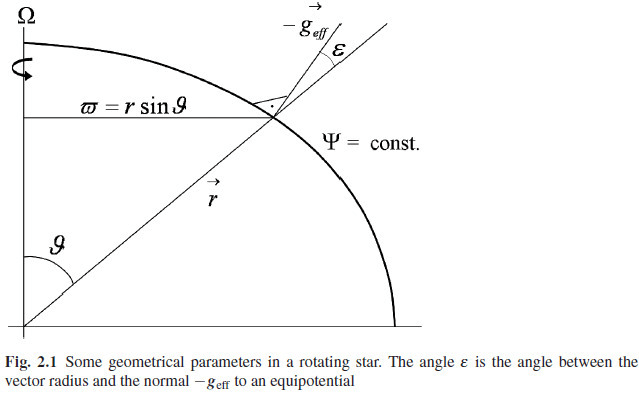
\includegraphics[width=(0.9\textwidth),height=(\textheight-11mm),keepaspectratio]{rotequi}
\caption{Geometrical parameters in rotating star.}
\end{figure}

Considerando la rotazione costante, cio\'e come corpo rigido, l'equazione del moto diventa
\begin{align*}
&\frac{1}{\rho}\nabla P=-\nabla\phi+\frac{1}{2}\Omega^2\nabla(r\sin{\theta})^2\\
&\vec{g}=-\nabla\phi=-\frac{Gm(r)}{r^2}\frac{\vec{r}}{r}
\end{align*}

Introduco un potenziale di rotazione
\begin{equation*}
-\nabla V=\Omega^2(r\sin{\theta})\Rightarrow V=-\frac{1}{2}\Omega^2(r\sin{\theta})^2
\end{equation*}

quindi l'equazione di Poisson diventa

\begin{align*}
&\nabla^2\Psi=4\pi G\rho-2\Omega\\
&\Psi=\phi+V
\end{align*}

e (barotropic stars) l'equazione di equilibrio idrostatico
\begin{equation*}
\frac{1}{\rho}\nabla P=-\nabla\Psi=g_{eff}
\end{equation*}

La forza centrifuga al polo \'e nulla quindi la superficie \'e un equipotenziale di $\frac{GM}{R_p}$, $R(\theta)$ \'e determinato da
\begin{equation*}
\frac{GM}{R(\theta)}+\frac{1}{2}\Omega^2R^2\sin^2{\theta}=\frac{GM}{R_p}
\end{equation*}

\clearpage

\subsection{Fluido in rotazione}

\begin{definition}{Parametro di deformazione}
Rapporto tra l'accelerazione centrifuga e l'accelerazione di gravit\'a: $u$.

\end{definition}

Definisco come parametro per descrivere la deformazione di un fluido autogravitante in rotaziane il rapporto tra l'attrazione gravitazionale e la forza centrifuga all'equatore
\begin{align*}
&u=\frac{\omega^2R^3}{GM}&\intertext{In termini di energia rotazionale e gravitazionale}\\
&E_{Rot}=\frac{1}{5}MR^2\omega^2\\
&E_{Gra}=\frac{3}{5}\frac{GM^2}{R}&\intertext{quindi}\\
&\frac{E_{Rot}}{E_{Gra}}=\frac{1}{3}\frac{\omega^2R^3}{GM}=\frac{1}{3}u\\
&u=\frac{3}{4}\frac{\omega^2}{\pi G \rho}&\intertext{per un corpo omogeneo}
\end{align*}

\subsection{Forma di equilibrio: argomento di Newton.}

Ellissoide di rotazione con semi-assi maggiori $a$ e minore $b=a\sqrt{1-e^2}$, $e$ \'e l'eccentricit\'a.

\begin{figure}[!ht]
\centering
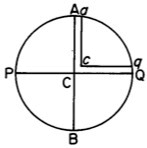
\includegraphics[width=(0.4\textwidth),height=(\textheight-11mm),keepaspectratio]{PEwell}
\caption{Colonne di fluido polare ed equatoriale.}
\end{figure}

Per densit\'a costante:
\begin{align*}
&ag_{eq}(1-u)=bg_{Pol}&\intertext{Primo membro: all'equatore l'accelerazione gravitazionale \'e diluita dall'accelerazione centrifuga (in corpo omogeneo sono proporzionali ad r). Il rapporto fra le due \'e uguale al valore sulla superficie.}\\
&ag_{eq}-a^2\omega^2=g_{Polo}a\sqrt{1-e^2}\\
&\epsilon=\frac{R_{eq}-R_{Polo}}{\exv{R}}=1-\sqrt{1-e^2}\approx\frac{e^2}{2}\\
&=1-\frac{b}{a}&\intertext{$\uparrow$ schiacciamento ai poli}\\
&\frac{g_{Polo}}{g_{eq}}=1+\frac{1}{5}\epsilon+O(\epsilon^2)&\intertext{quindi}\\
&(1-u)=(1-\epsilon)(1+\frac{1}{5}\epsilon)+O(\epsilon^2)\\
&=1-\frac{4}{5}\epsilon+O(\epsilon^2)&\intertext{da cui segue la relazione di Newton:}\\
&\epsilon=\frac{5}{4}u
\end{align*}

\clearpage

\subsection{MacLaurin spheroids}

Chiamo
\begin{align*}
&E_g=\frac{1}{2}\int\rho\Phi\,dV&\intertext{In caso di simmetria sferica: $\frac{d\Phi}{dr}=\frac{Gm(r)}{r^2}$}\\
&\chi=\frac{\omega^2}{2\pi G\rho}
\end{align*}

\begin{align*}
&e^2=\frac{a^2-b^2}{a^2}&\intertext{Along the series of increasing eccentricity $L$ and $E_g$ vary monotonically.}
\end{align*}

If we start with liquid selfgraviting body and feed in angular momentum $L$ also $\omega$ increases and e increses until $e\geq0.9299$ then $\omega$ decreses since moment of inertia increses faster than $\omega$. Before this, at $e=0.8127$, the McLaurin spheroid become unstable: the sequence of configuration shows a bifurcation and we have the Jacobi tri-axial ellipsoid (Jacobi ellipsoid of same mass and angular momentum has lower energi $E=E_g+E_{Rot}$)

\begin{figure}[!ht]
\centering
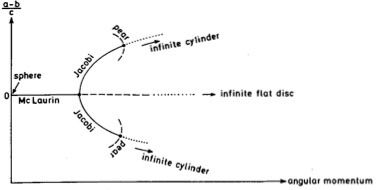
\includegraphics[width=(\textwidth),height=(\textheight-11mm),keepaspectratio]{McL2J}
\caption{Sequence of McLaurin and Jacobian equilibrium configurations of rotating incompressible fluid. a,b,c are 3 axis of an ellipsoid. Solid lines indicate dinamically or secularly stable configurations.}
\end{figure}

If there is a mechanism like friction which can transform macroscopic energy into heat spheroid become ellipsoid: the transition take place on the time-scale of friction.

\begin{figure}[!ht]
\centering
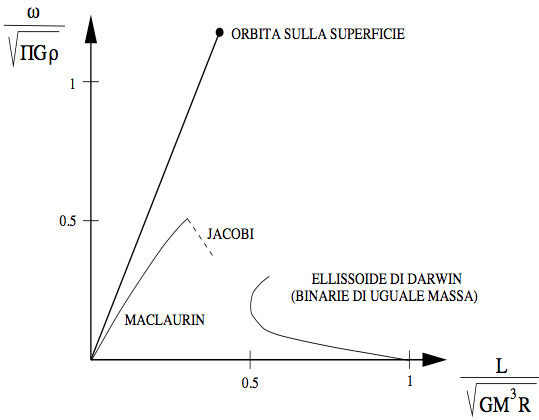
\includegraphics[width=(\textwidth),height=(\textheight-11mm),keepaspectratio]{Eq-shape}
\caption{Relazione $\omega-L$ per figure di equilibrio.}
\end{figure}

\clearpage


\chapter{Teorema del viriale: relazioni statistiche.}
\PartialToc

\section{Teorema del viriale}

\subsection{Thermal/kinetic energy}

\begin{align*}
&K=\int_0^R\overbrace{(+\frac{3}{2}\frac{K}{\mu m_u}T)}^{v^2}\rho 4\pi r^2\,dr\\
&=\overline{+\frac{3}{2}\frac{K}{\mu m_u}T}M\approx\SI{5e48}{\erg}
\end{align*}

\subsection{Teorema del viriale: equilibrio idrostatico.}

\begin{align*}
&\frac{1}{2}\TtwoDy{t}{I}=2K+\Omega\\
&2K=\sum_im_iv_i^2=\sum_i\scap{p_i}{v_i}&\intertext{$\scap{p_i}{v_i}$ measure rate of momentum transfer hence must be related to Pressure}\\
&P=\frac{1}{3}\int_pn(\vec{p})\scap{p}{v}d^3p&\intertext{confrontando le ultime due equazioni si ha:}\\
&2K=3\int_VP\,dV=3\int_M\frac{P}{\rho}\,dm(r)
\end{align*}

Il teorema del viriale si riscrive
\begin{align*}
&\frac{1}{2}\TtwoDy{t}{I}=\int_M\frac{3P}{\rho}\,dm(r)+\Omega&\intertext{Per equilibrio idrostatico}\\
&\frac{1}{2}\TtwoDy{t}{I}=0
\end{align*}

\subsection{$\gamma$-law equation of state.}

Se vale una relazione del tipo \mblock{P=(\gamma-1)\rho u} (per i gas ideali monoatomici con \mblock{\gamma=\frac{5}{3}}, \mblock{P=\frac{2}{3}\rho u})
\begin{equation*}
2K=3(\gamma-1)\int u\,dm
\end{equation*}

$K=E_i$ solo per $\gamma=\frac{5}{3}$: l'energia cinetica \'e uguale all'energia interna totale solo in determinate circostanze.

Il teorema del viriale si riscrive
\begin{equation*}
3(\gamma-1)E_i+\Omega=0
\end{equation*}

e scrivendo l'energia totale $W=E_i+\Omega$ ottengo la relazione esplicita tra energia totale ed energia potenziale gravitazionale per stelle idrostatiche in cui vale la relazione \mblock{P=(\gamma-1)\rho u}
\begin{equation*}
W=\frac{3\gamma-4}{3(\gamma-1)}\Omega
\end{equation*}



\subsection{Gravitational energy.}

Prendo un elemento di massa unitaria a distanza r: la sua energia potenziale dovuta alla massa entro r \'e $-\frac{Gm}{r}$. Quindi l'energia potenziale sommata su tutti gli elementi di massa $dm$ della stella \'e
\begin{equation*}
E_g=-\int_0^M\frac{Gm}{r}\,dm
\end{equation*}

L'energia $-E_g(>0)$ \'e l'energia necessaria ad espandere tutti gli strati a infinito: \'e l'energia liberata quando la stella si forma per contrazione di una gas rarefatto.



\subsection{Internal energy for ideal gas}

Per un gas ideale
\begin{align*}
&\frac{P}{\rho}=\frac{R}{\mu}T=(c_P-c_v)T=(\gamma-1)c_vT=\frac{2}{3}u&\intertext{$\uparrow$ ho usato: $\frac{R}{\mu}=c_P-c_v$. Per un gas monoatomico: $\gamma=\frac{c_P}{c_v}=\frac{5}{3}$ e $u=c_vT$ \'e l'energia interna del gas per unit\'a di massa}
\end{align*}


\subsection{Kinetic energy of the gas.}

\begin{align*}
&dE_k=\frac{3}{2}KT\,dN=\frac{3}{2}RT\,dm\\
&=\frac{3}{2}(c_P-c_V)T\,dm&\intertext{$dN$ \'e il numero di molecole nell'elemento di massa.}\\
&dU=c_VT\,dm&\intertext{quindi ricavo una relazione tra energia cinetica totale delle particelle di gas per unit\'a di massa ed energia interna per unit\'a di massa:}\\
&E_i=\frac{3}{2}(\gamma-1)U
\end{align*}


\subsection{Virial theorem for ideal monoatomic gas in hydrostatic equilibrium}

Il teorema del viriale connette due serbatoi di energia stellare.

\begin{align*}
&\int_0^M\frac{Gm}{r}\,dm=3\int_0^M\frac{P}{\rho}\,dm&\intertext{Il lato sinistro dell'equazione \'e $-E_g$: se la stella si espande/contrae $-E_g$ diminuisce/aumenta (valida per tempi grandi rispetto a $t_{hyd}$). $\uparrow$ deriva dalla seconda equazione fondamentale in forma Lagrangiana moltiplicata per $4\pi r^3$ integrata tra 0 ed M e la relazione $\downarrow$}\\
&\int_0^M4\pi r^3\frac{\partial P}{\partial m}\,dm\\
&=[4\pi r^3P]_0^M-\int_0^M12\pi r^2\frac{\partial r}{\partial m}P\, dm&\intertext{$\uparrow$ ho usato P(M)=0. Seconda equazione F. (equilibrio idrostatico): $\downarrow$}\\
&\frac{\partial P}{\partial m}=-\frac{Gm}{4\pi r^4}\\
&\frac{P}{\rho}=\frac{2}{3}u&\intertext{con $E_i=\int_0^Mu\,dm$:}\\
&E_g=-2E_i
\end{align*}


\subsection{Stima temperatura media.}

Star of uniform temperature and density composed of monoatomic ideal gas. The internal energy density is
\begin{align*}
&U=\frac{3}{2}nkT=\frac{3}{2}\rho\frac{N_AkT}{\mu}\si{\erg\per\cubic\cm}&\intertext{$\mu$ is the mean molecular weight per ion or atom}\\
&P=nkT=\frac{\rho N_AkT}{\mu}\\
&E_i=VU=\frac{3}{2}\frac{MN_AkT}{\mu}&\intertext{il teorema del viriale in questo caso ci dice che $E_i=-\frac{\Omega}{2}$, ($\gamma=\frac{5}{3}$)}\\
&\Omega=-\frac{3}{5}\frac{GM^2}{R}\\
&T=\num{4.09e6}\mu(\frac{M}{\msun{}})\expy{\frac{2}{3}}\rho\expy{\frac{1}{3}}\si{\kelvin}
\end{align*}



\subsection{Teorema del viriale per equazione di stato generale.}

Definisco parametro $\zeta$

\begin{align*}
&\zeta u=3\frac{P}{\rho}&\intertext{Gas ideale:}\\ &\zeta=3(\gamma-1)\xrightarrow{\gamma=\frac{5}{3}}2&\intertext{Pure photon gas:}\\
&P=\frac{1}{3}aT^4, u\rho=aT^4, \zeta=1
\end{align*}

Se $\zeta$ \'e costante nella stella ho una forma pi\'u generale del teorema del viriale
\begin{equation*}
\zeta E_i+E_g=0
\end{equation*}

\subsection{Coupling between $E_i$, $E_g$ and total energy.}

A change in total energy of the configuration is connected with change of its internal energy and with expansion or shrinking:
\begin{equation*}
W=E_i+E_g=(1-\zeta)E_i=\frac{\zeta-1}{\zeta}E_g
\end{equation*}

A gas of finite temperature must radiate
\begin{align*}
&L+\frac{dW}{dt}=0\\
&L=(\zeta-1)\frac{dE_i}{dt}=-\frac{\zeta-1}{\zeta}\frac{dE_g}{dt}
\end{align*}

Ho visto che $\dot{E_g}<0$ per contrazioni di tutti gli strati sferici e per un gas ideale l'equazione precedente da 
\begin{align*}
&L=-\frac{1}{2}\dot{E_g}=\dot{E_i}&\intertext{cio\'e met\'a dell'energia liberata dalla contrazione \'e irradiata nell'universo l'altra met\'a usata per scaldare la stella ($L>0,\dot{E_i}>0$)}
\end{align*}

Stars have negative specific heat: si scaldano mentre perdono energia.

\section{Kelvin-Helmholtz time-scale}

Definisco il tempo caratteristico per l'evoluzione di una stella in collasso: 
\begin{align*}
&L\approx|\frac{dE_g}{dt}|\\
&\tau_{KH}=\frac{E_i}{L}\propto\frac{|E_g|}{L}&\intertext{approssimando rozzamente $E_g$:}\\
&|E_g|\approx\frac{G\overline{m}^2}{\overline{r}}\approx\frac{GM^2}{2R}\\
&t_{KH}\approx\frac{GM^2}{2RL}
\end{align*}
\index{Kelvin-Helmholtz time-scale.}

For the sun $L=3.827 *10^{33}erg/s$ so $t_{KH}\approx1.6*10^7\,yr$.

There are phases in a stellar life when $E_g$ is the main energy source then the star evolves on Kelvin-Helmholtz time-scale.


In any case
\begin{align*}
&\TDy{m}{T}=-\frac{T}{P}\frac{Gm(r)}{4\pi r^4}\nabla\\
&\nabla=\TDly{P}{T}
\end{align*}

\chapter{Energy conservation and energy flux.}
\PartialToc


\section{Third basic equation of stellar structure}

\subsection{Prima legge della termodinamica. Conservazione energia interna.}

If stresses reduce to pure pressure \mblock{P_{ij}=P\delta_{ij}}
\begin{equation*}
\TDy{t}{q}=\TDy{t}{E}+P\TDof{t}(\frac{1}{\rho})=\TDy{t}{E}+P\TDof{t}V
\end{equation*}

equivalent form under asumption 1) $P(\rho,T)$, 2) $E(\rho,T)$, 3) No composition change due to nuclear reaction.

La prima legge della termodinamica esprime la conservazione dell'energia interna (per unit\'a di volume).

Le equazioni equivalenti utilizzando gli esponenti adiabatici $\Gamma_i$

\begin{align*}
&\Gamma_1=\Dcvar{\TDly{\rho}{P}}{Ad},\ \Gamma_3-1=\Dcvar{\TDly{\rho}{T}}{Ad},\\ &\frac{\Gamma_2-1}{\Gamma_2}=\Dcvar{\TDly{P}{T}}{Ad}
\end{align*}

\begin{align*}
&\TDy{t}{\ln{T}}=\frac{\Gamma_2-1}{\Gamma_2}\TDy{t}{\ln{P}}+\frac{\TDy{t}{q}}{c_PT}\\
&\TDy{t}{\ln{P}}=\Gamma_1\TDy{t}{\ln{\rho}}+\frac{\rho(\Gamma_3-1)}{P}\TDy{t}{q}
\end{align*}

Per un gas perfetto $\gamma=\frac{c_P}{c_v}=\Gamma_i$.


\subsection{Flusso di energia locale}
Chiamo $l(r)$ il flusso di energia totale verso l'esterno da una sfera di raggio $r$: energia per sec.

In $l(r)$ sono compresi il trasporto di energia attraverso radiazione, conduzione, convezione: are included only those fluxes that require a temperature gradient.

\begin{figure}[!ht]
\centering
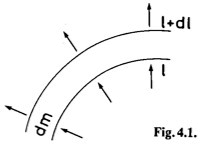
\includegraphics[width=(0.5\textwidth),height=\textheight,keepaspectratio]{localEF}
\caption{Contributo $dl$ da parte dello strato $dm$ fra $r$ e $r+\,dr$.}
\end{figure}

\subsection{Stationary case: only nuclear reaction contributes to $dl$.}

\begin{align*}
&dq=(\epsilon-\PDy{m}{l})\,dt&\intertext{Stato stazionario: il flusso di energia non modifica lo stato termodinamico del gas}\\
&dl=4\pi r^2\rho\epsilon\,dr=\epsilon\,dm\\
&\PDy{m}{l}=\epsilon
\end{align*}

\subsection{Non stationary case: also internal energy and exchange of work contribute to $dl$.}

\begin{align*}
&dq=(\epsilon-\PDy{m}{l})\,dt&\intertext{$\uparrow$ heat added per unit mass to the shell in the interval $dt$. Dalla prima legge della termodinamica ($dq=\,du+P\,dV$) ho:}\\
&\epsilon-\PDy{t}{u}-P\PDy{t}{v}=\epsilon-\PDy{t}{u}+\frac{P}{\rho^2}\PDy{t}{\rho}=\PDy{m}{l}&\intertext{In termini di $T$ e $P$ ho:}\\
&dq=c_P\,dT-\frac{\delta}{\rho}\,dP,\\
&(\delta=-\Dcvar{\PDly{T}{\rho}}{P}=\frac{T}{v}\Dcvar{\PDy{T}{v}}{P})&\intertext{ e quindi:}\\
&\PDy{m}{l}=\epsilon-c_P\PDy{t}{T}+\frac{\delta}{\rho}\PDy{t}{P}&\intertext{$\uparrow$ third basic equation of stellar structure.}
\end{align*}



\subsection{Considero la variazione di stato del gas: contributo alla luminosit\'a negativo/positivo.}

Definisco una funzione che contiene il contributo alla variazione di $l(r)$ per unit\'a di massa dovuta alla variazione dello stato termodinamico del gas

\begin{align*}
&\epsilon_{gas}=-\TDy{t}{q}=-T\PDy{t}{s}=-c_P\PDy{t}{T}+\frac{\delta}{\rho}\PDy{t}{P}\\
&=-c_PT(\frac{1}{T}\PDy{t}{T}-\frac{\nad}{P}\PDy{t}{P})\\
&\delta=-\Dcvar{\PDly{T}{\rho}}{P}=\frac{T}{v}\Dcvar{\PDy{T}{v}}{P}\\
&\nad{}=\Dcvar{\PDly{P}{T}}{s}=\frac{P\delta}{T\rho c_P}
\end{align*}

Surface luminosity of an expanding star can be smaller than energy produced in central core by nuclear reaction ($\epsilon>0$) since part of it is used to expand the star ($\epsilon_g<0$).

\subsection{Complete local energy equation}
La terza equazione fondamentale della struttura stellare \'e
\begin{align*}
&\PDy{m}{l}=\epsilon-c_P\PDy{t}{T}+\frac{\delta}{\rho}\PDy{t}{P}\\
&=\epsilon-\epsilon_{\nu}+\epsilon_g\\
&L_{\nu}=\int_0^M\epsilon_{\nu}\,dm&\intertext{$\uparrow$ neutrino luminosity. Condizioni al contorno:}\\
&l(0)=0\\
&l(R)=L
\end{align*}

\subsection{Energy conservation: total energy.}

Energia totale di una stella
\begin{align*}
&W=E_{Macro}+E_g+E_i+E_n&\intertext{$E_{Macro}$ is the kinetic energy of radial motion, $E_n$ is the nuclear energy content of the whole star. Energy balance:}\\
&\TDof{t}(E_{Macro}+E_g+E_i+E_n)+L+L_{\nu}=0&\intertext{Ottengo la stessa equazion $\uparrow$ integrando l'equazione locale rispetto a $dm$:}\\
&\int_0^M\,dm(\PDy{m}{l})=\int_0^M\,dm(\epsilon-\epsilon_{\nu}+\epsilon_{gas})\\
&\int\PDy{m}{l}=L,\quad\int-\epsilon_{\nu}\,dm=-L_{\nu},\\
&\int\epsilon\,dm=-\dot{E_n}&\intertext{Considero l'integrale di $\epsilon_{gas}$:}\\
&\int\,dm[-\PDy{t}{u}+\frac{P}{\rho^2}\PDy{t}{\rho}]=-\TDy{t}{E_i}-\TDy{t}{E_g}&\intertext{Il primo termine nelle parentesi quadre da}\\
&\int\,dm(-\PDy{t}{u})=-\TDy{t}{E_i}&\intertext{Per riconoscere il secondo derivo rispetto al tempo $E_g$ e uso il teorema del viriale \mblock{E_g=-2E_i=-\int\,dm3\frac{P}{\rho}}:}\\
&\dot{E_g}=-3\int_0^M\frac{\dot{P}}{\rho}\,dm+3\int_0^M\frac{P}{\rho^2}\dot{\rho}\,dm&\intertext{(Ricordo che:)}\\
&(-E_g=\int_0^M\frac{Gm}{r}\,dm=3\int_0^M\frac{P}{\rho}\,dm)&\intertext{Dalla condizione di equilibrio idrostatico ($E_{Macro}=0$) ricavo:}\\
&-3\int_0^M\frac{\dot{P}}{\rho}\,dm=\int_0^M4\pi r^3\PDy{m}{\dot{P}}\,dm\\
&=4\int_0^M\frac{Gm}{r}\frac{\dot{r}}{r}\,dm=4\dot{E_g}
\end{align*}

Per recuperare il termine $E_{Macro}$ devo usare l'equazione del moto
\begin{equation*}
\frac{1}{4\pi r^2}\PtwoDy{t}{r}=-\PDy{m}{P}-\frac{Gm}{4\pi r^4}
\end{equation*}
invece dell'equazione dell'equilibrio idrostatico.




\section{Time-scale consideration: sequenza principale, stelle pulsanti}

\subsection{Nuclear time-scale}

I consider a star balancing its energy loss by release of nuclear energy.

\begin{align*}
&\tau_n=\frac{E_n}{L}&\intertext{$E_n$ is the energy reservoir from which nuclear energy can be released. Hydrogen burning release:}\\
&Q=6.8*\sci{18}\,erg\,g^{-1}&\intertext{for a sun of only hydrogen}\\
&E_n=Q\msun=1.25*\sci{52}\,erg,\\
&\lsun=4*\sci{33}\,erg/\,sec\\
&\tau_n=3*\sci{18}s=\sci{11}\,yr
\end{align*}

\subsection{Ordine di grandezza termini energy equation}

Condizione $\tau_n\gg\tau_{KH}\gg\tau_{Hyd}$.

\begin{align*}
&|\PDy{m}{l}|\approx\frac{L}{M}\approx\frac{E_i}{\tau_{KH}M}\\
&\epsilon\approx\frac{L}{M}\approx\frac{E_n}{M\tau_n}\approx\frac{E_i}{\tau_{KH}M}&\intertext{$\uparrow$: $L$ \'e la stessa sia che la fonte di energia sia nucleare sia che sia l'energia potenziale gravitazionale. Introduco un tempo che caratterizza una determinata fase evolutiva della stella:}\\
&|c_P\PDy{t}{T}|\approx\frac{c_PT}{\tau}\approx\frac{E_i}{\tau M}\\
&|\frac{\delta}{\rho}\PDy{t}{P}|\approx\frac{c_PT}{\tau}\approx\frac{E_i}{\tau M}&\intertext{$\uparrow$ ho usato:}\\
&P=\frac{\rho}{\mu}RT,\ \delta=\frac{T}{v}\Dcvar{\PDy{T}{v}}{P},\\
&c_P=\Dcvar{\PDy{T}{q}}{P}=\Dcvar{\PDy{T}{u}}{P}+P\Dcvar{\PDy{T}{v}}{P}
\end{align*}

\subsection{Stelle di sequenza}

Nel caso $\tau\gg\tkh$ posso trascurare le derivate rispetto al tempo $(|\epsilon_g|\ll\epsilon)$, the energy equation becomes
\begin{align*}
\PDy{m}{l}=\epsilon&\intertext{This happens,ie, if H and He consumption sturns the evolution: $\tau=\tau_n$ and we have mechanical and thermal equilibrium}
\end{align*}

\subsection{Stelle pulsanti}

Nel caso $\tau\ll\tkh$ 
\begin{align*}
&|c_P\PDy{t}{T}|\approx|\frac{\delta}{\rho}\PDy{t}{P}|&\intertext{e cancellarsi a vicenda visto che $\TDy{t}{q}\approx0$ (change nearly adiabatic): a relatively small deviation from strictly adiabatic change can still be of order $\epsilon$. $\epsilon_g$ cannot be neglected.}
\end{align*}

For a pulsationg stars with \mblock{\tau=\thydro\ll\tkh} the variable luminosity is not due to changes of $\epsilon$ but $\epsilon_g$.


\part{Trasporto radiativo. Stabilit\'a rispetto a perturbazioni dello stato interno. Trasporto convettivo.}
\chapter{Transport of energy by radiation and conduction.}
\PartialToc

\section{Radiative transfer}

Photons emitted thermally in hotter regions and absorbed in cooler transfer energy. The effectiveness depends on thermal gradient and ability of the photons to travel freely (among others).The rate of radiative energy transport will be proportional to gradient of fourth power of T.

The reduction of intensity of a beam of photons passing through matter is
\begin{align*}
&\TDy{x}{I}=-\overline{\kappa}\rho I\\
&dI_{\nu}=-\kappa_{\nu}\rho I_{\nu}\,ds
\end{align*}



\subsection{Absorption/scattering coefficients}

$\kappa_{\nu}$ is the mass absorption coefficient: it includes processes of absorption and scattering. In star's interior where matter is completely ionized the bulk of scattering occurs from Thomson scattering by free electrons whereas in cool atmosphere may be due to molecular scattering.

\begin{align*}
&dI_{\nu}=-\kappa_{\nu a}\rho I_{\nu}\,ds\\
&dI_{\nu}=-\kappa_{\nu s}\rho I_{\nu}\,ds\int_{\Omega'}p(\cos{\theta'})\frac{d\Omega'}{4\pi}
\end{align*}
$p(\cos{\theta'})$ is the scattering phase function which gives angular distribution of scattered energy removed from the beam: for Rayleigh scattering $p(\cos{\theta'})=1+\cos^2{\theta'}$.

\subsection{Emission of photons: kirchhoff law}

$j_{\nu}(\theta)$ represents the true emission of radiation of freq. $\nu$ per unit frequency interval in direction $\theta$ per unit solid angle from each gram of stellar matter. The specific intensity of radiation at angle $\theta$ will be increased by

\begin{align*}
&dI_{\nu}(\theta)=j_{\nu }\rho\,ds&\intertext{assumption that stellar interior is in local thermodynamic equilibrium: matter radiates spontaneously in stellar interior as it would in thermodynamic equilibrium: stellar matter is assumed to have temperature T and assumption of local thermodynamic equilibrium is that matter at T radiates exactly as it would if it were in surroundings in thermodynamic equilibrium at same T  :}\\
&I(\theta)=\frac{c}{4\pi}u\ (+\frac{3}{3\pi}H\cos{\theta})&\intertext{sine T gradient is small compared to mean free path of photns in stellar interior the photons are absorbed at same temperature they are emitted. Condition for LTE:}\\
&j_{\nu}=\kappa_{\nu a}\frac{cu_{\nu}}{4\pi}=\kappa_{\nu a}B_{\nu}(T)&\intertext{kirchhoff law}
\end{align*}

Part of the emissions contained in kirchhoff law is spontaneous emission resulting only from T and part is induced emission. The induced emission comes from atomic transitions caused by radiation field and produes radiation with same freq. and moving in same pencil of direction as incident radiation.

\begin{usefull}{Fraction of total emission that is spontaneous}

\begin{align*}
&\frac{\text{Spontaneous}}{\text{Total}}=\frac{N_iA_{ij}}{N_iA_{ij}+N_iB_{ij}u_{\nu_{ij}}}\\
&=\frac{1}{1+(B_{ij}/A_{ij})u_{\nu_{ij}}}
&\intertext{where $\frac{1}{4\pi}N_iA_{ij}$ is a spontaneous transition rate per unit solid angle, $\frac{1}{4\pi}N_iB_{ij}u_{\nu_{ij}}$ is the rate of photons emission (in same direction of incident photons) per unit solid angle, induced by encounters of atoms in state i with photons $\nu_{ij}$}\\
&\frac{\text{Spontaneous}}{\text{Total}}=1-\exp{-\frac{h\nu}{kT}}&\intu{Qm radiation theory requires that this ratio of spontaneous to total emission in local thermodynamic equilibrium apply to any mechanism of true absorption}
\end{align*}

there are mechanism other than transitions between atomic states that represent true emission/absorption: ionization is a true absorption, whereas inverse process is true emission.

\begin{definition}{Induced ionization/recombination}
QM can be show that radiative recombination of ion and electrons with emission of a photon $\nu_{ij}$ can be induced by presence of second photon $\nu_{ij}$.
\end{definition}

One reaches a ratio of spontaneous emission for radiative recombination to total emission by radiative recombination equal to that for atomic transitions.



\end{usefull}

\subsection{Slightly anisotropic radiation field in stellar interior}

One must be cautious to avoid making a mistake in extending properties of radiation computed for condition of local thermodynamic equilibrium to slightly anisotropic radiation field in stellar interior.

If deviation from strict thermodynamic equilibrium occur emission must be separated into two terms: spontaneous emission is still determined by T of matter and the source function is $B_{\nu}(T)$ whereas the induced emission is proportional to actual specific intensity of radiation $I_{\nu}(\theta)$ instead of $B_{\nu}(T)$:
\begin{equation*}
j_{\nu}(\theta)=\kappa_{\nu a}(1-\exp{-\frac{h\nu}{kT}})B_{\nu}(T)+\kappa_{\nu a}\exp{-\frac{h\nu}{kT}}I_{\nu}(\theta)
\end{equation*}

\subsection{Energy introduced into pencil by scattered photons}

Energy scattered per unit solid angle into pencil moving in direction $(\theta,\phi)$ from a pencil in direction $(\theta',\phi')$:
\begin{equation*}
j_{\nu,scat}=\kappa_{\nu s}\frac{1}{4\pi}\int_0^{\pi}\int_0^{2\pi}p(\theta,\phi,\theta',\phi')I_{\nu}(\theta',\phi')\sin{\theta'}\,d\theta'\,d\phi'
\end{equation*}

\subsection{Energy balance: equation of transfer}

We consider a cylinder with axis along $(\theta,\phi)$
\begin{align*}
&\Dcvar{\TDy{t}{Q}}{top}=-I_{\nu}(r+dr,\theta)\,d\Omega&\intu{power exiting from top}\\
&\Dcvar{\TDy{t}{Q}}{bot}=I_{\nu}(r,\theta)\,d\Omega&\intu{power entering from bottom}\\
&\Dcvar{\TDy{t}{Q}}{abs}=-(\kappa_{\nu a}+\kappa_{\nu s})\rho I_{\nu}(r,\theta)\,dl\,d\Omega&\intu{power per unit area absorbed during transit of cylinder}\\
&\Dcvar{\TDy{t}{Q}}{emis}=\kappa_{\nu a}\rho\,dl[(1-\exp{-\frac{h\nu}{kT}})B_{\nu}(T)\\
&+\exp{-\frac{h\nu}{kT}}I_{\nu}(\theta)]\,d\Omega+\kappa_{\nu s}\rho\,dl\frac{d\Omega}{4\pi}*\\
&\iint p(\theta,\phi,\theta',\phi')I_{\nu}(r,\theta',\phi')\sin{\theta'}\,d\theta'\,d\phi'
\end{align*}

From energy conservation \mblock{\Dcvar{\TDy{t}{Q}}{tot}=0}:

\begin{align*}
&I_{\nu}(r+dr,\theta)-I_{\nu}(r,\theta)=\PDy{r}{I_{\nu}}\,dr=\\
&-(\kappa_{\nu a}+\kappa_{\nu s})\rho I_{\nu}(r,\theta)\,dl\\
&+(1-\exp{-\frac{h\nu}{kT}})B_{\nu}(T)\kappa_{\nu a}\rho\,dl\\
&+\exp{-\frac{h\nu}{kT}}I_{\nu}(\theta)\kappa_{\nu a}\rho\,dl\\
&+\kappa_{\nu s}\frac{\rho\,dl}{4\pi}*\int p(\theta,\phi,\theta',\phi')I_{\nu}(r,\theta',\phi')\,d\Omega'
\end{align*}

Using \mblock{dr/dl=\cos{\theta}} and \mblock{\kappa_{\nu a}^*=\kappa_{\nu a}(1-\exp{-\frac{h\nu}{kT}})}:

\begin{align*}
&\frac{1}{\rho\,dl}\PDy{r}{I_{\nu}}\,dr=\frac{1}{\rho}\PDy{r}{I_{\nu}}\cos{\theta}\\
&=-(\kappa_{\nu a}^*+\kappa_{\nu s})I_{\nu}(r,\theta)+\kappa_{\nu a}^*B_{\nu}(T)\\
&+\kappa_{\nu s}\frac{1}{4\pi}*\int p(\theta,\phi,\theta',\phi')I_{\nu}(r,\theta',\phi')\,d\Omega'
\end{align*}

It's the desired equation of radiative transfer for plane parallel atmosphereunder LTE.

\subsection{Photon gas}

Assuming polar axis parallel to direction of net flow.

\begin{align*}
&P_r=\frac{1}{3}\intzi{}\frac{h\nu}{c}cn(\nu)\,d\nu\\
&I(\theta)\,d\Omega=cu(\theta)\,d\Omega&\intu{$u(\theta)\,d\Omega$ represent energy density of radiation moving at angle $\theta$ in $d\Omega$}\\
&H=\int\,d\Omega I(\theta)\cos{\theta}&\intertext{stellar radiation is anisotropic in radial direction}\\
&I(\theta)\approx\frac{c}{4\pi}u+\frac{3}{4\pi}H\cos{\theta}+\ldots&\intu{the second term is much smaller than the first}
\end{align*}

\begin{figure}[!ht]
\centering
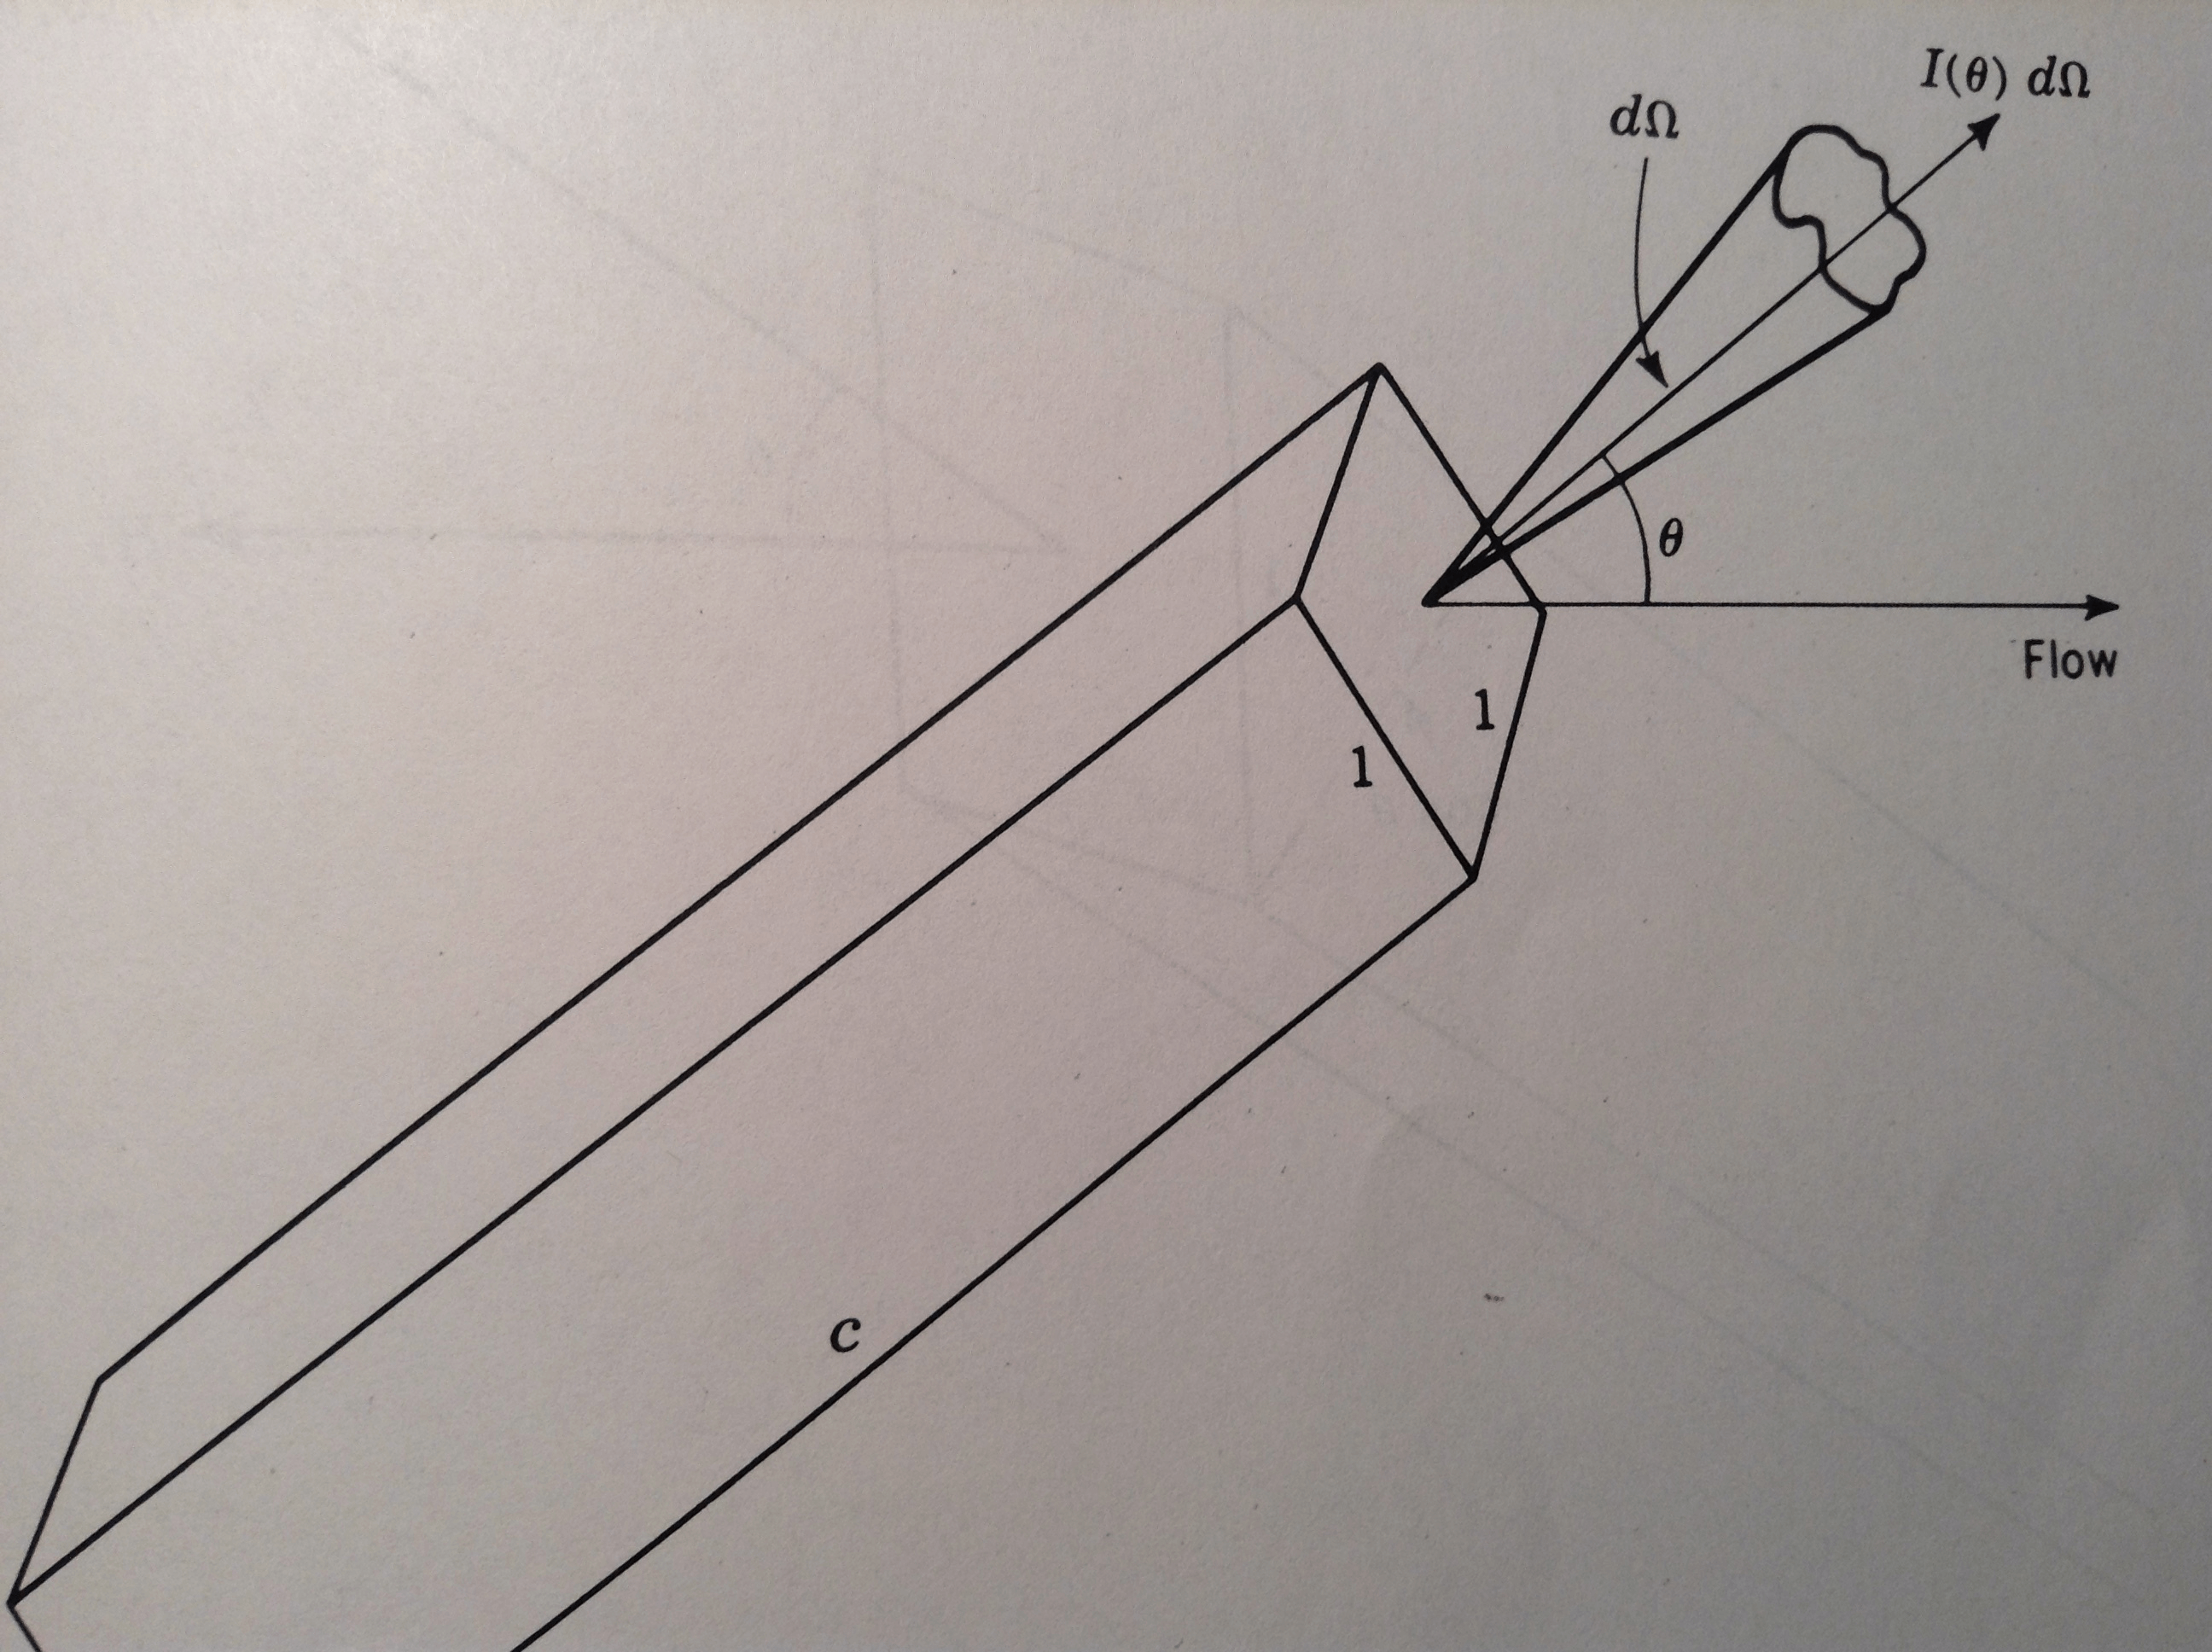
\includegraphics[width=\textwidth,height=0.9\textheight,keepaspectratio]{intensity}
\caption{$I(\theta)\,d\Omega$ is the energy flux moving in direction $\theta$}\label{fig:energyflux}
\end{figure}

\begin{figure}[!ht]
\centering
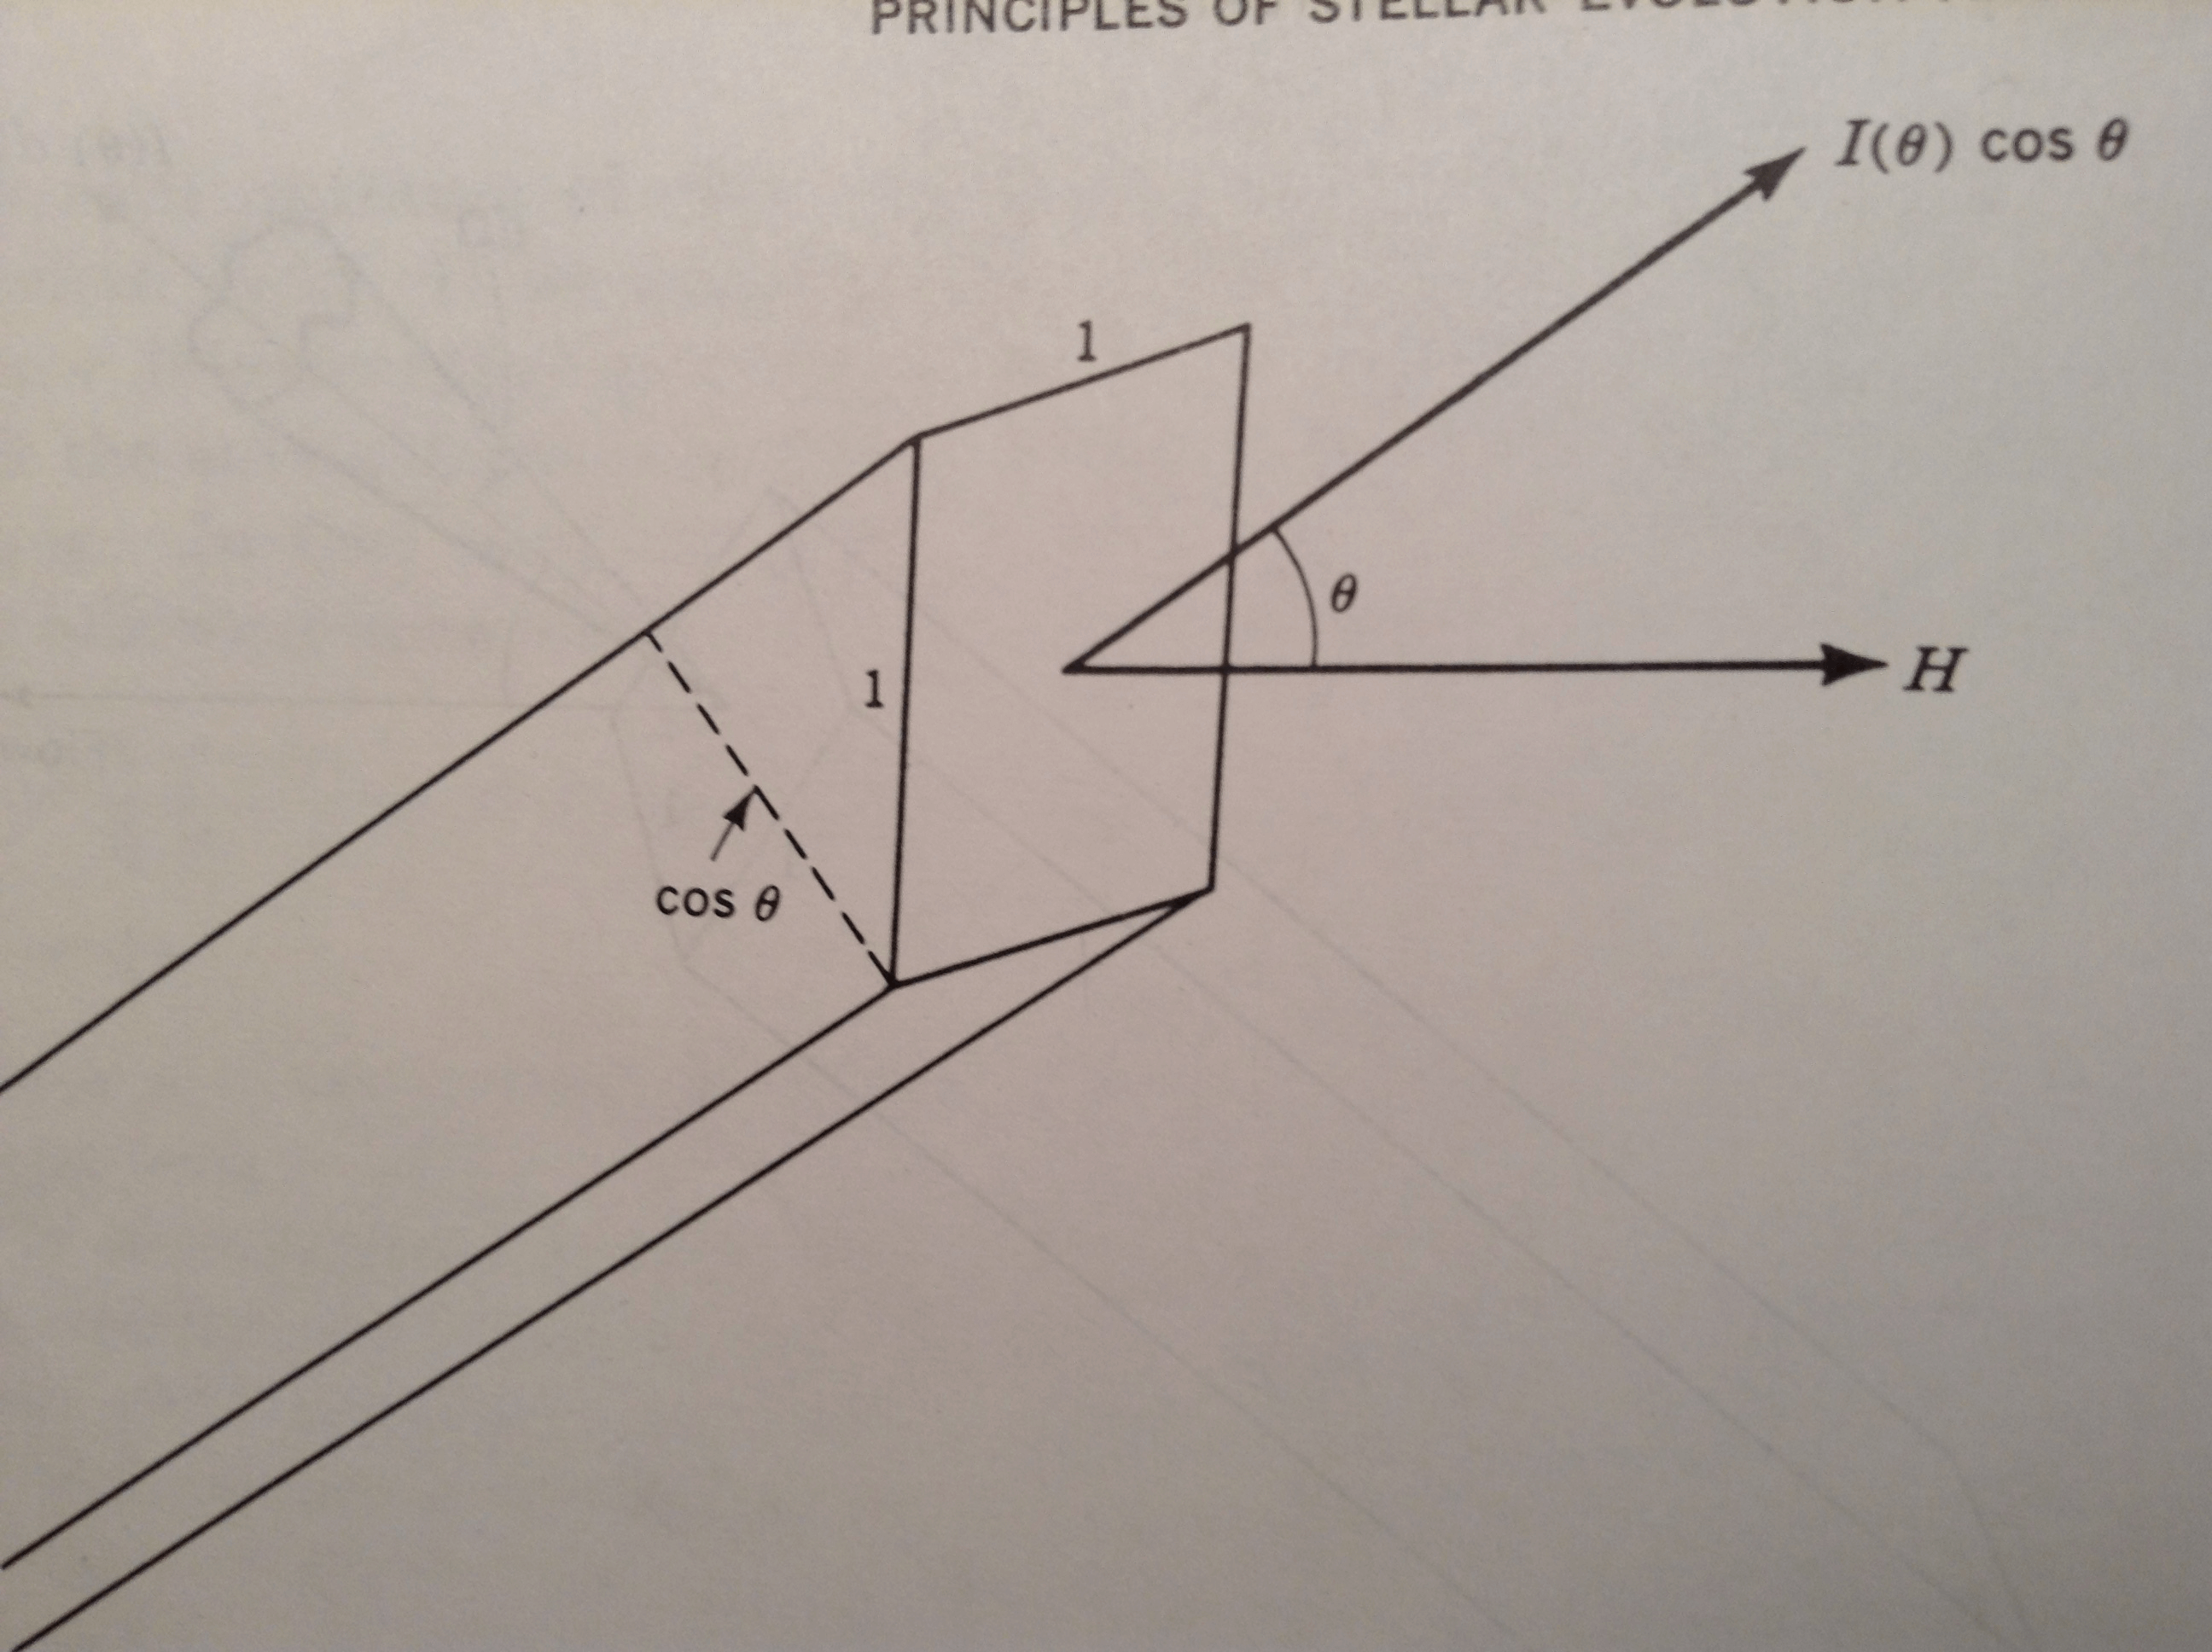
\includegraphics[width=\textwidth,height=0.9\textheight,keepaspectratio]{flux}
\caption{Energy flux with $I(\theta)\,d\Omega$ with associated energy flow per unit area normal to polar axis H equals to $I(\theta)\,d\Omega\cos{\theta}$.}\label{fig:energyflux}
\end{figure}

\begin{figure}[!ht]
\centering
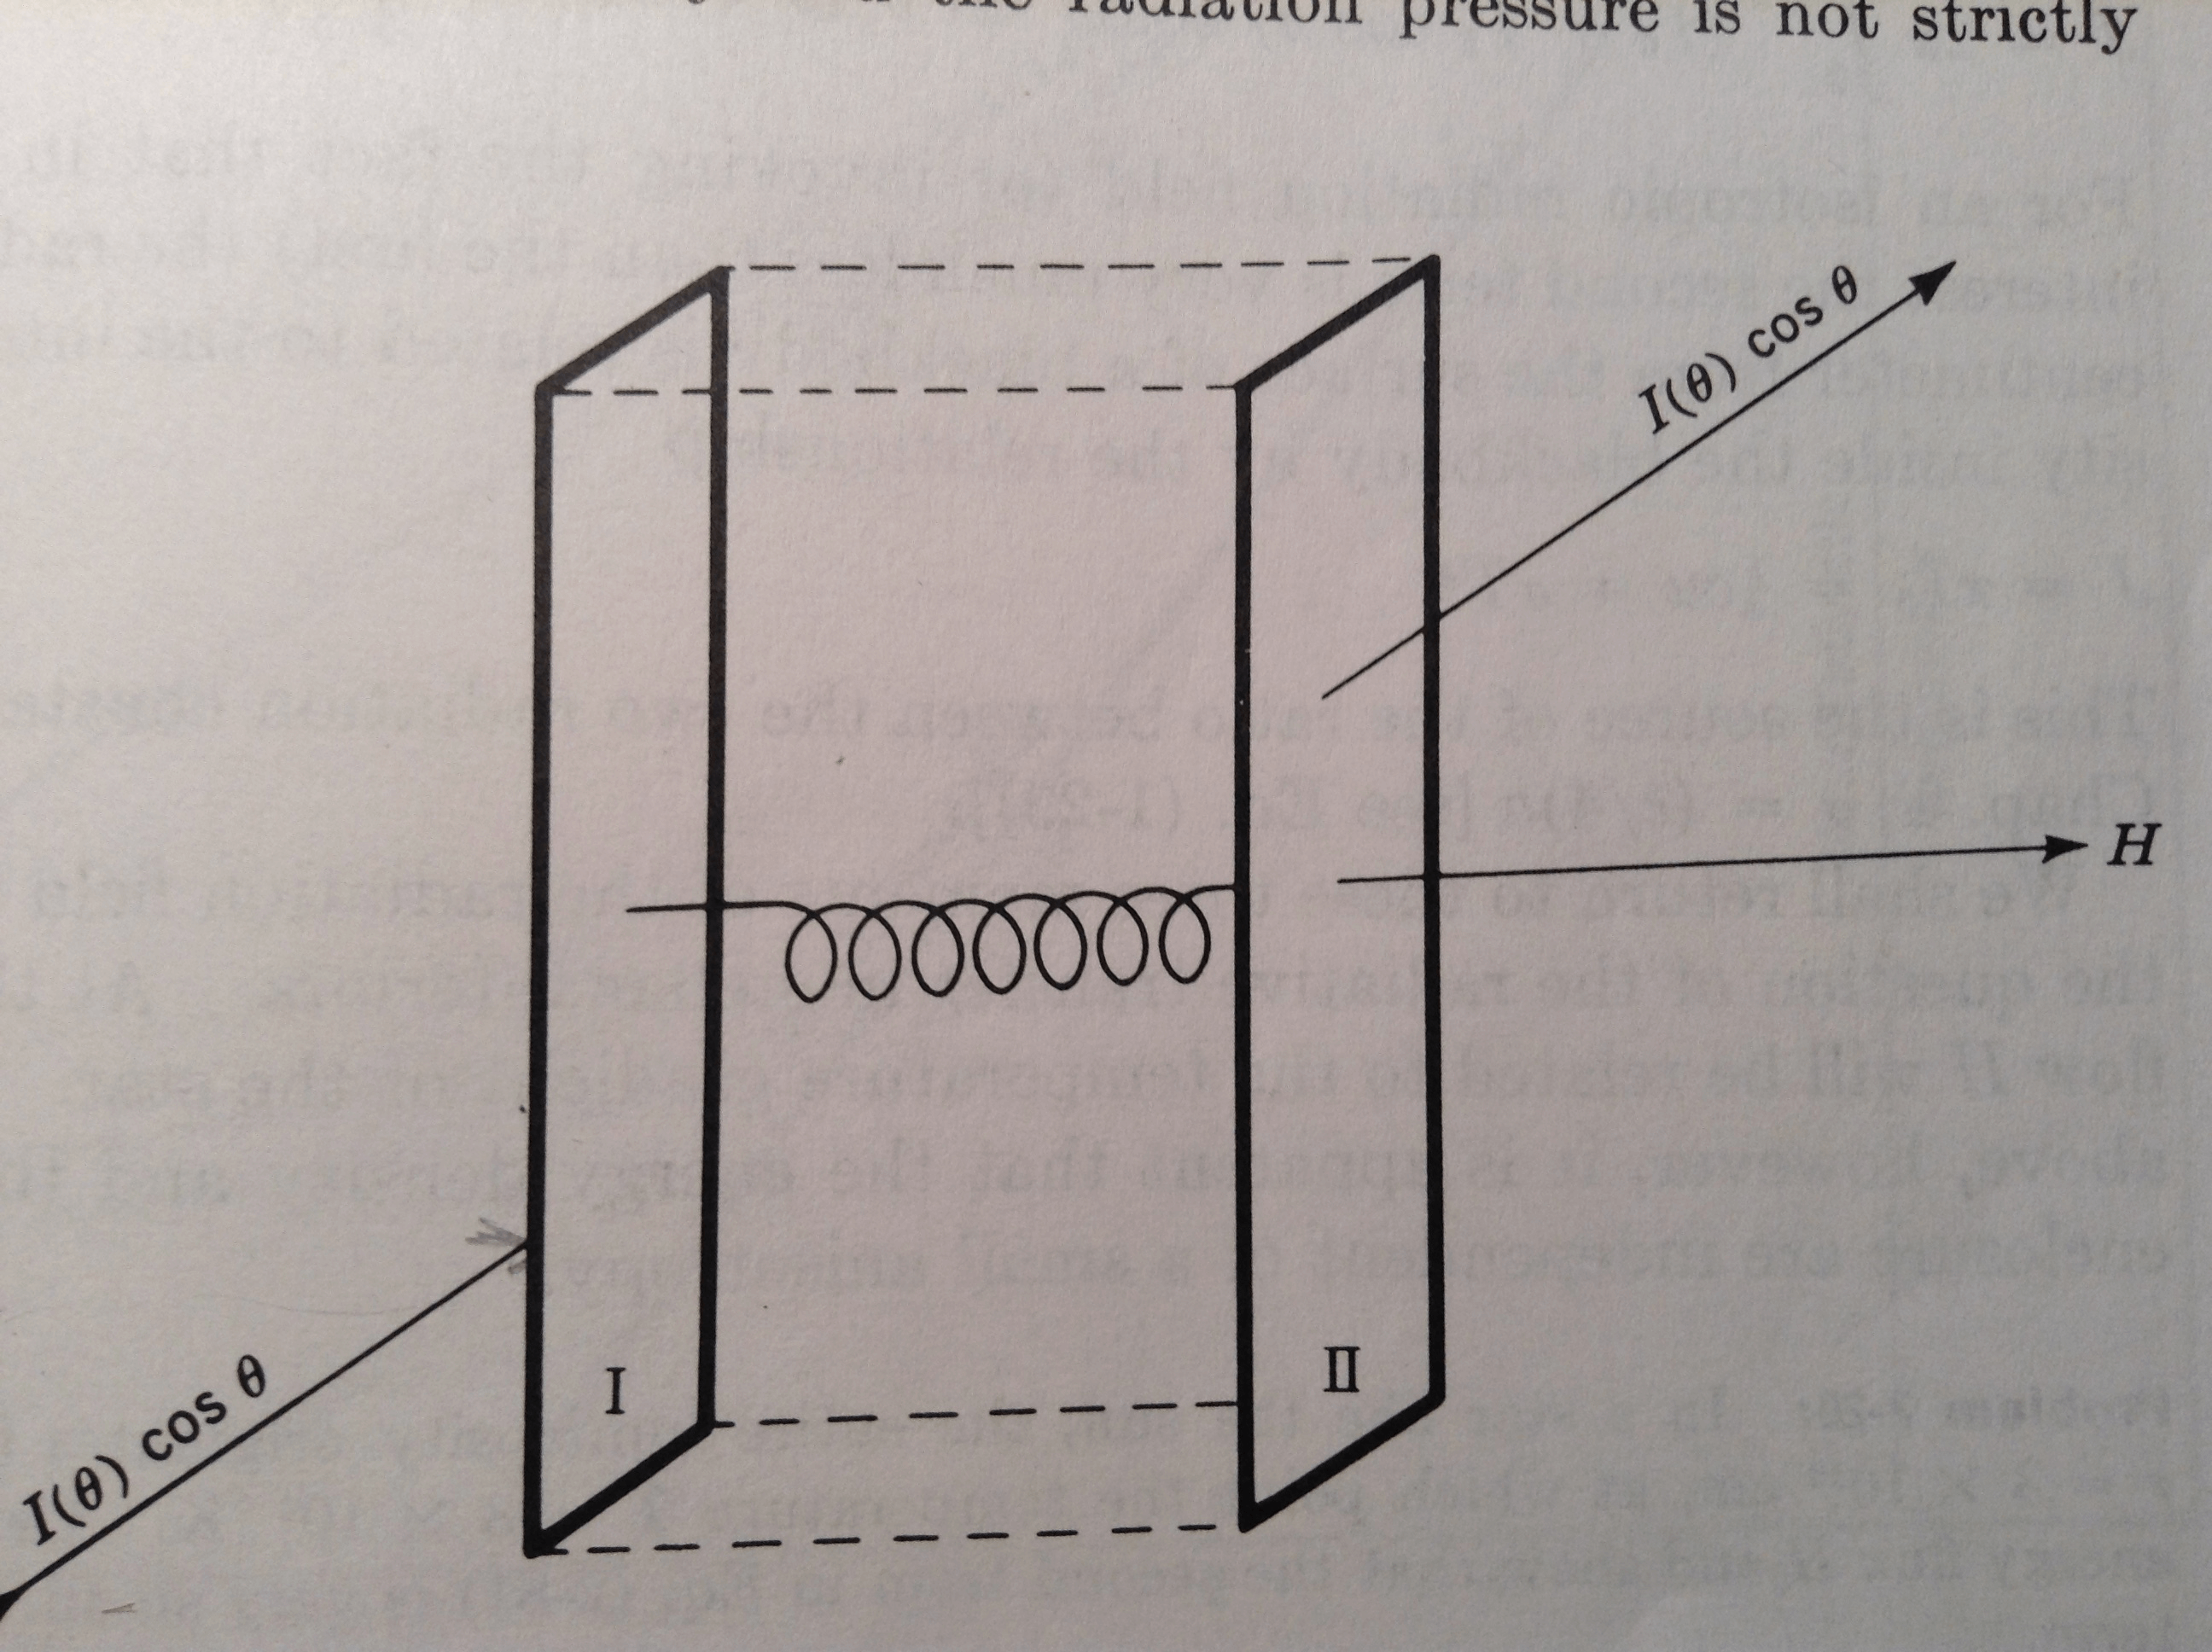
\includegraphics[width=\textwidth,height=0.9\textheight,keepaspectratio]{radpres}
\caption{The radiation pressure is the resulting compressional force on the spring.}\label{fig:radpressure}
\end{figure}

\clearpage

\subsection{Energy flow per unit area in terms opacity and temperature gradient}

\begin{usefull}{A quantity per unit dimension}
Describe characteristic properties of a unitary dimensional entity: mass of unitary surface base cylinder is $\rho\,dl$.
\end{usefull}

What is desired for computation of stellar structure is an equation of transfer that gives energy flow per unit area in terms of an averaged opacity and temperature gradient.

Multiplying the radiative equation transport by $\cos{\theta}$ and dividing by total mass of cylinder of unit area $\rho\,dl$

\begin{align*}
&\frac{1}{\rho}\PDy{r}{I_{\nu}}\cos^2{\theta}\,d\Omega=\frac{1}{\rho}\PDof{r}\int I_{\nu}\cos^2{\theta}\,d\Omega=\frac{c}{\rho}\PDy{r}{P_{\nu}}\\
&\int (\kappa_{\nu a}^*+\kappa_{\nu s})I_{\nu}(r,\theta)\cos{\theta}\,d\Omega=(\kappa_{\nu a}^*+\kappa_{\nu s})H_{\nu}\\
&\int \kappa_{\nu a}^*B_{\nu}(T)\cos{\theta}\,d\Omega=0
&j_{\nu s}=0&\intu{assuming p contains only even power of cosine between the scattering beams}
\end{align*}

The result of these operations on equation of transfer is

\begin{equation*}
\frac{c}{\rho}\PDy{r}{P_{\nu}}=-(\kappa_{\nu a}^*+\kappa_{\nu s})H_{\nu}(r)
\end{equation*}
even in case of a slightly anisotropy $P_{\nu}=\frac{1}{3}u_{\nu}$. The total heat flux per unit area is
\begin{equation*}
H=\intzi{}H_{\nu}\,d\nu=-\frac{c}{3\rho}\intzi{}\frac{1}{\kappa_{\nu a}^*+\kappa_{\nu s}}\TDy{r}{u_{\nu}}\,d\nu
\end{equation*}

Since $u_{\nu}$ is function only of T in thermodynamic equilibrium \mblock{\TDy{r}{u_{\nu}}=\TDy{T}{u_{\nu}}\TDy{r}{T}}
\begin{align*}
&H=-\frac{c}{3\rho}\intzi{}\frac{1}{\kappa_{\nu a}^*+\kappa_{\nu s}}\TDy{T}{u_{\nu}}\TDy{r}{T}\,d\nu&\intertext{which multiplied/divided by}\\
&\intzi{}\TDy{T}{u_{\nu}}\,d\nu=\TDof{T}\intzi{}u_{\nu}\,d\nu=4aT^3&\intertext{becomes:}\\
&H=-\frac{4ac}{3\rho}T^3\TDy{r}{T}\frac{\intzi{}\frac{1}{\kappa_{\nu a}^*+\kappa_{\nu s}}\TDy{T}{u_{\nu}}\,d\nu}{\intzi{}\TDy{T}{u_{\nu}}\,d\nu}&\intertext{and since in thermodynamical equilibrium $B_{\nu}$ differs from $u_{\nu}$ by a constant we define:}\\
&\frac{1}{\kappa}=\frac{\intzi{}\frac{1}{\kappa_{\nu a}[1-\exp{-\frac{h\nu}{kT}}]+\kappa_{\nu s}}\TDy{T}{B_{\nu}}\,d\nu}{\intzi{}\TDy{T}{B_{\nu}}\,d\nu}
\end{align*}

The correction factor for induced emission diminuisce l'assorbimento a basse energie \mblock{h\nu<kT}, the weighting factor $\TDy{T}{B_{\nu}}$ physically mean that the photon frequencies most important for radiative transfer are those for which the difference in the product of photon number density times photon energy between two points of slighly different T is maximal.

\begin{usefull}{Radiative heat flux in stellar interior}
\begin{equation*}
H=F(r)=\frac{l}{4\pi r^2}=\frac{4ac}{3\rho\kappa}T^3\TDy{r}{T}
\end{equation*}
\end{usefull}


\subsection{Euristic derivation}
todo

\subsection{Properties of stars in radiative equilibrium}

\begin{align*}
&\TDy{r}{P_r}=-\frac{\kappa\rho}{4\pi cr^2}l(r)\\
&\TDy{r}{l(r)}=4\pi r^2\rho\epsilon\\
&\TDy{P}{P_r}=\frac{\kappa l(r)}{4\pi G m(r)}\\
&\eta(r)=\frac{\overline{\epsilon_r}}{\epsilon}=\frac{l(r)/m(r)}{L/M}\\
&\TDy{P}{P_r}=\frac{L}{4\pi cGM}\kappa\eta\\
&P_r(r)=\frac{L}{4\pi cGM}\int_0^{P(r)}\kappa(r)\eta(r)\,dP\\
&=\frac{L}{4\pi cGM}P(r)\overline{\kappa\eta}
\end{align*}


\begin{usefull}{Ratio of radiation pressure to total pressure}
The ratio of radiation pressure to total pressure at a point inside a star in radiative equilibrium is proportional to averaged value of $\kappa\eta$ for regions exterior to point r anfd the average is taken by $p(r)$.

\end{usefull}

\begin{usefull}{Luminosity formula}
For stellar center
\begin{align*}
&\beta_c=\frac{P_g}{P}\\
&L=\frac{4\pi cGM(1-\beta_c)}{\overline{\kappa\eta}}
\end{align*}
\end{usefull}

\begin{usefull}{Standard model: non-degenerate polytrope of index 3}
Constant $\beta$ yield the non degenerate polytrope of index 3
\begin{align*}
&P=K\rho\expy{\frac{n+1}{n}}\\
&P_g=\frac{N_ak}{\mu}\rho T=\beta P,\ P_r=\frac{1}{3}aT^4=(1-\beta)P\\
&T=(\frac{N_ak}{\mu}\frac{3}{a}\frac{1-\beta}{\beta})\rho\expy{\frac{1}{3}}&\intu{closure relation??}\\
&P=K\rho\expy{\frac{4}{3}}&\intertext{constancy of $\beta$ depends on constancy of $\kappa\eta$: $\kappa$ increases by several order of magnitude from center to surface and $\eta$ decreases by several order of magnitude}\\
&
\end{align*}
\end{usefull}

\begin{usefull}{Mass-luminosity relationship for main-sequence stars}
\begin{align*}
&T_c\propto M\expy{\frac{2}{3}}\overline{\rho}\expy{\frac{1}{3}}=\frac{M}{R}\\
&\TDy{r}{T}\propto\frac{T_c}{R}\\
&L\propto R^2\frac{(M/R)^3}{M/R^3}\frac{M/R}{R}=M^3
\end{align*}
\end{usefull}

\section{Radiative energy transport.}

\subsection{Mean-free path of a photon.}

\begin{align*}
&l_{Ph}=\frac{1}{\kappa\rho}&\intertext{$\kappa$ is a mean absorption coefficient: Radiative cross section per unit mass averaged over frequency $(\kappa\approx1\,cm^2/g)$. Per il sole:}\\
&l_{Ph}^{\odot}=2\,cm\ll\rsun&\intertext{$\uparrow$ con $\rhosun=\frac{3\msun}{4\pi\rsun^3}=14g/cm^3$. Stellar matter is very opaque.}
\end{align*}

\subsection{Stefan-Boltzman law.}

L'energia interna in una corpo nero di volume V \'e $U=Vu(T)$ dove $u(T)$ \'e la densit\'a di energia dei fotoni:
\begin{align*}
&\frac{du}{u}=4\frac{dT}{T}\\
&u=aT^4
\end{align*}


\subsection{Radiation pressure}

Tutte le volte che un atomo emette/assorbe un fotone perde/guadagna quantit\'a di moto e dato che un atomo emette in maniera isotropa il momento netto \'e nullo una volta mediato su molte emissioni.

I processi di assorbimento non sono isotropicamente distribuiti dato il flusso uscente di energia per $cm^2$ per sec F: solo una frazione $\kappa$ del flusso di momento $\frac{F}{c}$ \'e assorbita dalla materia. Il trasferimento da parte della radiazione di momento alla materia per $cm^3$ per sec, cio\'e la forza esercitata dalla radiazione \'e $\kappa H \frac{1}{c}$.

Un elemento di volume $dS\,dr$ subisce per effetto dell'assorbimento della radiazione una variazione d'impulso $dq$, nel caso un fotone venga assorbito la variazione del flusso uscente \'e $dF<0$

The distribution of photons over over different quantum states with energies $\epsilon_k=\hbar\omega_k$ (large volume $\omega_k\to\omega$) 
\begin{align*}
\overline{n_k}=\frac{1}{\exp{\frac{\hbar\omega}{KT}}-1}
\end{align*}

Moltiplicando il numero di stati nel dato range di frequenze per la distribuzione di Plank (numero di occupazione) ottengo il numero di fotoni e l'energia radiativa nel range di frequenza

\begin{align*}
&dN_{\omega}=\frac{V}{\pi^2c^3}\frac{\omega^2\,d\omega}{\exp{\frac{\hbar\omega}{KT}}-1}\\
&dE_{\omega}=\frac{V\hbar}{\pi^2c^3}\frac{\omega^3\,d\omega}{\exp{\frac{\hbar\omega}{KT}}-1}
\end{align*}


\begin{align*}
&dq=-(n_{\nu}\,dSc\,dt)*(\kappa\rho\,dr)*\frac{h\nu}{c}&\intertext{Il primo termine \'e il numero di fotoni pasanti per superficie $dS$ in tempo $dt$, il secondo \'e la probabilit\'a d'assorbimento attraverso spessore $dr$, il terzo \'e la quantit\'a di moto di ogni fotone.}\\
&dP_r=\TDy{S}{F}=\TDof{S}\TDy{t}{q}\\
&=-\int \,d\nu n_{\nu}c\kappa_{\nu}\rho\,dr\frac{h\nu}{c}\\
&F_{\nu}=n_{\nu}ch\nu,\\
&\TDy{r}{P(Rad)}=-\int\,d\nu\frac{F(Rad)}{c}\kappa_{\nu}\rho&\intertext{In condizioni di LTE posso confrontare $\uparrow$ con}\\
&P_{\nu}=\frac{1}{3}u_{\nu},\ P(Rad)=\frac{1}{3}aT^4&\intertext{e ricavare il gradiente di temperatura necessario per il flusso di energia $F(Rad)$:}\\
&\TDy{r}{T}=-\frac{3\kappa\rho l(r)}{16\pi acT^3r^2}
\end{align*}


\subsection{Local thermodynamic equilibrium}


The thermodynamic theory of radiation is valid only when system is adiabatically enclosed (all parts at same temperature): many physical system though they aren't in thermodynamic equilibrium yet they permit introduction of a temperature to describe local properties: if $\kappa_{\nu}$, $j_{\nu}$ are the coefficient of absorption emission of an element mass we have




\section{Radiative transport: photon diffusion.}


\subsection{Stima del gradiente di temperatura: Local thermal equilibrium.}

Close to local thermal equilibrium
\begin{equation*}
\frac{\Delta T}{\Delta r}\approx\frac{T_c-T_0}{R}|_{\odot}\approx1.4\sci{-4}\,K/cm
\end{equation*}

The radiation field at a given point is emitted from a small nearly adiabatic surrounding:
\begin{align*}
&\Delta T\approx l_{Ph}(\TDy{r}{T})\approx3\sci{-4}K&\intertext{Relative anisotropy of radiation with $T=\sci{7}\,K$:}\\
&\frac{\Delta u}{u}\approx\frac{4T^3\Delta T}{T^4}=\frac{4\Delta T}{T}\approx\sci{-10}
\end{align*}

\subsection{Diffusion of Radiative energy.}

The radiation in stellar interior is very close to that of a black body but the small anisotropy carries the huge luminosity of star:

$\sci{-10}$ of the flux emitted from $1 cm^2$ of a black body at $T=\sci{7}K$ is $\sci{3}$ times larger than flux at solar surface ($6\sci{10}\,erg/cm^2/s$).

Radiative transport occurs because of surplus of outgoing radiation emitted by hotter marial below over the ingoing radiation emitted from less hot material above.

Since $l_{Ph}\ll\rsun$ radiative transport in stars can be treated as a diffusion process

\begin{align*}
&\vec{J}=-D\nabla n&\intertext{$\uparrow$ is the flux (diffusive) of particles per unit area per unit time between places of different particles densities,}\\
&D=\frac{1}{3}vl_P&\intertext{is the diffusion coefficient determined by mean velocity and mean free path of particles.}\\
&|F|=\frac{1}{3}cl_{Ph}\PDy{r}{u},\quad\PDy{r}{u}=4aT^3\PDy{r}{T}&\intertext{$\uparrow$  ipotesi di simmetria sferica}\\
&F=-\frac{4ac}{3}\frac{T^3}{\kappa\rho}\PDy{r}{T}&\intertext{$\uparrow$ can be interpeted as heat conduction equation $F=-k_{Rad}\nabla T$. Ricavo il gradiente di T sostituendo $l=4\pi r^2F$:}\\
&\PDy{r}{T}=-\frac{3}{16\pi ac}\frac{\kappa\rho l(r)}{r^2T^3}\\
&\PDy{m}{T}=-\frac{3}{64\pi^2 ac}\frac{\kappa l(r)}{r^4T^3}&\intertext{$\uparrow$ these equations become invalid when one approaches the surface: $l_{Ph}$ becoms large (Large optical depth $d\tau=\rho\kappa\,dr$: stellar interior).}
\end{align*}

\subsection{Rosseland mean for opacity}

Considero la dipendenza dalla frequenza per radiazione $[\nu,\nu+\,d\nu]$

\begin{align*}
&F_{\nu}=-D_{\nu}\nabla U_{\nu},\quad D_{\nu}=\frac{1}{3}cl_{\nu}=\frac{c}{3\kappa_{\nu}\rho}\\
&u_{\nu}=\frac{4\pi}{c}B(\nu,T)=\frac{8\pi h}{c^3}\frac{\nu^3}{\exp{\frac{h\nu}{KT}}-1}&\intertext{B is the Plank function for intensity of black body radiation}\\
&\vec{F}=-[\frac{4\pi}{3\rho}\int_0^{+\infty}\frac{1}{\kappa_{\nu}}\PDy{T}{B}\,d\nu]\nabla T&\intertext{Definisco la media di Rosseland tramite:}\\
&\frac{1}{\kappa}=(\underbrace{\frac{acT^3}{\pi}}_{\int_0^{\infty}\PDy{T}{B}\,d\nu})^{-1}\int\frac{1}{\kappa_{\nu}}\PDy{T}{B}\,d\nu&\intertext{The rosseland mean favours the frequency ranges of maximum energy flux:}\\ &F_{\nu}=-(\frac{1}{\kappa_{\nu}}\PDy{T}{B})\frac{4\pi}{3\rho}\nabla T\\
&\kappa_{\nu}=X\kappa_{\nu}(H)+Y\kappa_{\nu}(He)&\intertext{$\uparrow$ opacity for given frequency for mixture of H and He.}
\end{align*}


\subsection{Stability condition for radiative equilibrium}

Consider the perturbation: I displace an element of matter in stellar interior upward by the distance $dr$, let's the element expand adiabatically until the pressure inside the element is in balance with the pressure of the surroundings.

\begin{figure}[!ht]
\centering
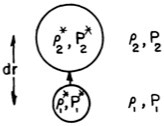
\includegraphics[width=(0.3\textwidth),height=(\textheight-11mm),keepaspectratio]{conv_stab}
\caption{Perturbation of radiative layer to test for stability against convection.}
\end{figure}

After the perturbation the density may differs now from that of the surroundings since internal density is determined by adiabatic transformation of the element
\begin{align*}
P_2=P_2^*,\quad\rho_2^*=\rho_1^*(\frac{P_2^*}{P_1^*})^{\frac{1}{\gamma}}&\intertext{where $\gamma=\frac{c_P}{c_v}$ is the ratio of specific heat and has the value $\frac{5}{3}$ for highly ionized gas}
\end{align*}

The pressure force exerted on that volume which the element occupies after its displacement and expansion has not be alterated by the perturbation, the gravitational force will be altered if the density within the element after the perturbation differs from that in the surroundings.

Condizione di stabilit\'a
\begin{align*}
\rho_2^*>\rho_2&\intertext{I can trasform this condition in a more practical one: sobstituting expression for the variables of surroundings and taking taylor's expansion of the quantities at higher position:}\\
-\frac{1}{\gamma}\frac{1}{P}\TDy{r}{P}<-\frac{1}{\rho}\TDy{r}{\rho}
\end{align*}

For the cases where the equation of state for an ideal gas hold I can take logarithimic derivative of $P=\frac{k}{\mu}\rho T$ and thus I can express density gradient in terms of temperature and pressure gradient:

\begin{align*}
-(1-\frac{1}{\gamma})\frac{T}{P}\underbrace{\TDy{r}{P}}_{\text{from HE}}>-\underbrace{\TDy{r}{T}}_{\text{from RE}}&\intertext{since both temperature gradient and pressure gradient are negative both sides of $\uparrow$ are positive. Right side contains absolute value of temperature gradient, left side contains the adiabatic temperature gradient (would represent temperature gradient if the temperature and pressure followed the adiabatic relationship through the layer).}
\end{align*}

For a layer to be stable against convection the actual temperature gradient must be lower in absolute value than the adiabatic temperature gradient.\index{Stability condiction against convection: Schwarzschild.}

The above condiction hold only in homogenous layers.


\section{Meccanismi che contribuiscono  all'opacit\'a.}

\subsection{Radiation and equilibrium}

\begin{definition}{Emission coefficient.}
\begin{align*}
&j_{\nu}=m\,d\omega\,dt\,d\nu&\intu{amount of radiant energy emitted: $j_{\nu}$ is the emission coefficient for frequency $\nu$.}
\end{align*}
\end{definition}

\begin{definition}{Einstein coefficients.}
\begin{itemize}
\item Spontaneous emission.

The probability that in a interval of time $dt$ an atom in an excited state n emits a quantum of energy $h\nu_{mn}$ in the solid angle $d\omega$ in absebce of external field is $A_{nm}\,d\omega\,dt$: this spontaneous emission take place uniformly in all direction.

\item Stimulated emission.

The probability that an excited atom in state n is stimulated by external field of radiation to emit a quantum $h\nu_{nm}$, in the direction $d\omega$, in time $dt$ is given by $B_{nm}I_{\nu_{nm}}\,d\omega\,dt$, where $I_{\nu_{nm}}$ is the intensity of radiation of frequency $\nu_{nm}$ at the point where the atom is located and in the direction $d\omega$: the induced emission of radiation by a given pencil of radiation take place in the same direction as incident pencil.

\end{itemize}

In condizioni di equilibrio termodinamico
\begin{equation*}
j_{\nu}=\kappa_{\nu}B_{\nu}(T)
\end{equation*}
where T is the (local) temperature.

If there are $N_m$ atoms in n-th state per unit volume
\begin{align*}
&\frac{A_{nm}}{B_{nm}}=\frac{2h\nu_{nm}^3}{c^2}\\
&\frac{N_mB_{mn}}{N_nB_{nm}}=\exp{\frac{h\nu_{nm}}{KT}}
\end{align*}

\end{definition}

Vedi Chandrasekhar pg 190

\subsection{Electron scattering.}

Lo scattering da parte di un elettrone di un'onda EM incidente ovvero, l'emissione di dipolo di un'elettrone oscillante indotta da un'onda elettromagnetica \'e equivalente all'assorbimento del fotone:
\begin{align*}
&\sigma_e=\frac{8\pi}{3}(\frac{e^2}{m_ec^2})^2=\SI{6.652e-25}{\square\cm}&\intu{Thomson cross-section, the associated opacity coefficient is due to combined effect of all electrons in a unit mass of gas}\\
&\kappa_{es}=\frac{\sigma_e}{\frac{\rho}{n_e}}=\frac{\sigma_e}{\mu_em_u}&\intertext{for totally ionized gas $\mu_e=\frac{2}{1+X}$:}\\
&\kappa_{es}=0.20(1+X)\si{\square\cm\per\gram}
\end{align*}

Electon scattering is important source of opacity in ionized gas not too dense. When degree of ionization drops ($T\leq\SI{e4}{\kelvin}$, in H-rich gas) the electron density become so small that  $\kappa_{es}$ is strongly reduced.

\subsubsection{Energetic photons: Effetto Compton.}

When photon energy becomes significant fraction of rest mass of electron $h\nu\geq0.1m_ec^2$ the exchange of momentum between photon and electron must be taken in account (Compton scattering): at high temperature since maximum of Plank function is at \mblock{h\nu=4.965 KT,\ KT\geq0.02m_ec^2} or $T\geq\SI{e8}{\kelvin}$: At high temperature the electron scattering opacity is reduced.

\subsection{Free-free absorption.}

A free electron cannot absorbs a photon because of momentum/energy conservation; it can happens if there is an EM with a close ion: it's the inverse process of bremsstrahlung. The derivation of absorption coefficient is a QM problem: an approximate calculation is the Kramer's law.

\subsubsection{Kramer's law.}

The absorption efficiency of the temporary electron-ion system is proportional to $Z_i^2\nu^{-3}$

\begin{align*}
&\kappa_{\nu}^{ff}\propto\frac{n_e}{\rho}\sum_in_iZ_i^2T\expy{-\frac{1}{2}}\nu^{-3}&\intu{cross-section of ion i:}\\
&\overline{v}=\sqrt{\frac{3KT}{m_e}}\\
&\Delta t\propto1/\overline{v}\propto T\expy{-\frac{1}{2}}&\intu{time of effective ion-electron coupling.}\\
&\sigma^{ff}_i\propto n_eT\expy{-\frac{1}{2}}Z_i^2\nu\expy{-3}&\intertext{the opacity coefficient follows by multiplying $\uparrow$ by $\frac{n_i}{\rho}$.}\\
\end{align*}

In a completely ionized gas $\frac{n_e}{\rho}=\frac{1}{\mu_em_u}=\frac{1+X}{2m_u}$.

\begin{align*}
&\kappa_{ff}\propto\rho T\expy{-\frac{7}{2}}\\
&\kappa_{ff}\propto\num{3.8e22}\rho T\expy{-\frac{7}{2}}\si{\square\cm\per\gram}
\end{align*}

We have to the into account of QM effects with the Gaunt factor.

\subsection{Bound-free, bound-bound absorption.}

\begin{itemize}
\item Bound-free absorption is the absorption of a photon by a bounded electron where the photon energy exceed ionization energy $\chi$. Classical consideration lead to formula of the Kramer form.
\item Bound-Bound absorption. Efficient because the absorption lines are broadened by collisions. Important for $T\leq\SI{e6}{\kelvin}$.
\item Bound-free absorption of negative hydrogen ion ($\chi=\SI{0.75}{\ev}$). Important in cool stars or solar atmosphere. The resulting opacity is sensitive to metallicity and temperature: the free electrons to make ion come from single ionized metals such as Na, K, Ca, Al.
\item Dust and molecules. In cool stars with $\teff\leq\SI{4000}{\kelvin}$ opacity from molecules and dust grain ($T\leq\SI{1500}{\kelvin}$) becomes dominant.
\end{itemize} 

\subsubsection{Negative H ion}

\subsection{Temperature-density diagram for the opacity.}

\begin{todo}{Temperature-density diagram for the opacity}
Schwarzschild pg 67-73
\end{todo}

\begin{figure}[!ht]
\centering
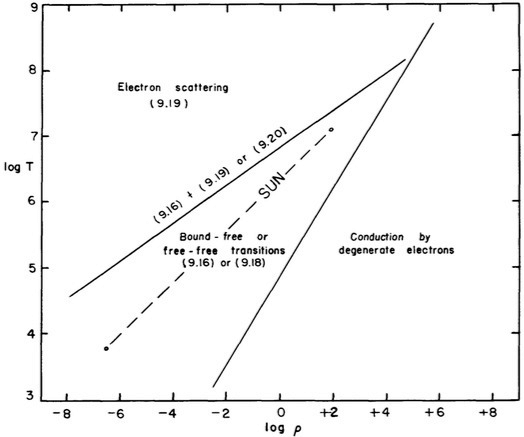
\includegraphics[width=(0.9\textwidth),height=(\textheight-11mm),keepaspectratio]{kappaqu}
\caption{Temperature-density diagram for the opacity.}
\end{figure}

\clearpage

\section{Relazione Massa-Luminosit\'a}

\subsection{Stability of thermal equilibrium}

Estimate of luminosity in the sun midway between center and surface.

\begin{align*}
&L_r=4\pi r^2\frac{4ac}{3}\frac{T^3}{\kappa\rho}\TDy{r}{T}&\intertext{$\uparrow$ radiative equilibrum plus crude estimates:}\\
&\kappa\rho\approx1cm,\quad T\approx10\sci{6}\,K&\intertext{taking for differnetial the difference I have:}\\
&L\approx6\sci{35}&\intertext{$\uparrow$ exceeds the luminosity of the sun by a factor 100.}
\end{align*}

How does the luminosity of a star depends on its mass?

\begin{align*}
&L_r=4\pi r^2\frac{4ac}{3}\frac{T^3}{\kappa\rho}\TDy{r}{T}&\intertext{$\uparrow$ radiative equilibrum plus crude estimates:}\\
&\rho\propto \frac{M}{R^3}&\intertext{introducing this proportionality in hydrostatic equilibrium equation $\downarrow$}\\
&\TDy{r}{P}=-\frac{Gm(r)\rho}{r^2}&\intertext{we find the dependence of representative pressure on the mass and radius $\downarrow$}\\
&P\propto\frac{M^2}{R^4}&\intertext{from equation of state for ideal gas, $T\propto\frac{P}{\rho}$, we have $\downarrow$}\\
&T\propto\frac{M}{R}&\intertext{introducing the proportinalities for T and P in radiative equilibrium equation we obtain:}\\
L\propto M^3
\end{align*}

\index{Mass-Luminosity relation: radiative equilibrium condition.}

The above estimates point out that the luminosity of a star is not determined by the rate of energy generation by nuclear process: only radiative equilibrium condition enters in the derivation.

The pressure force must counteract gravity according to HE equation: if the pressure have to be high enough for this porpuse the internal temperature must have certain relatively high values according to equation of state. The temperature gradient from hot internal zone to cold surface will cause a net radiation flux according to 
\begin{equation*}
l(r)=-4\pi r^2\frac{4ac}{3}\frac{T^3}{\kappa\rho}\TDy{r}{T}
\end{equation*}

The stength of this radiation flux will be fixed by radiative equilibrium condition irrespective of whether or not the the energy loss is compensate by nuclear energy production in the interior. If the energy loss by radiation at the surface is bigger the nuclear energy generation the suffers a net energy loss: this can made up from gravitational energy by contraction. During the contraction one half of the gravitational energy is available for radiation losses from surface, the other half go into increase of thermal energy. The contraction will stops when the over-all rate nuclear energy release is equal to radiative surface losses.


\subsection{Relazione massa luminosit\'a: limite di Eddington.}

Ipotesi:
\begin{itemize*}
\item Trasporto in superficie \'e radiativo conduttivo
\item $\kappa$ \'e approx costante
\item La pressione di radiazione fornisce un contributo dominante alla pressione totale
\end{itemize*}

Se la pressione di radiazione fornisce un contributo dominante $P\approx P_r$ ho
\begin{align*}
&\TDy{r}{P_r}=-\frac{\kappa_{\nu}}{c}\rho\frac{l(r)}{4\pi r^2}&\intertext{$\uparrow$ LTE}\\
&\PDy{r}{P}\approx\PDy{r}{P_r}=-\frac{Gm(r)\rho}{r^2}&\intertext{$\uparrow$ equilibrio idrodinamico}\\
&L=l(R)=GM\frac{4\pi c}{\kappa}&\intertext{Stimo il valore della costante di proporzionalit\'a fra massa e luminosit\'a nel caso di stelle massicce $\beta=\frac{P_g}{P}\approx0$:}\\
&\frac{L}{\lsun}\approx\sci{4}\frac{M}{\msun}&\intertext{$\uparrow$ \'e un limite superiore: limite di Eddington. Utile per studio dei nuclei galatticci. Utilizzando il modello di Eddington ($\beta=const$) invece ho:}\\
&\TDy{r}{P_r}=(1-\beta)\TDy{r}{P}=-(1-\beta)\frac{Gm(r)}{r^2}\rho&\intertext{quindi}\\
&L\approx[1-\beta(M)]\sci{4}(\frac{M}{\msun})\lsun&\intertext{Per piccole masse $\beta\approx1$ e quindi $1-\beta(M)\propto M^2$ ho:}\\
&L\propto M^3
\end{align*}

\subsection{Tempo di vita per oggetti che si avvicinano al limite di Eddington}

Energia disponibile
\begin{align*}
E_d=\alpha Mc^2&\intertext{$\alpha\approx0.01$ per reazioni nucleari, $\alpha\approx1$ per oggetti massicci.}
\end{align*}

Stimo il tempo di vita sulla base dell'energia disponibile
\begin{align*}
&T_{Max}=\frac{E_d}{L}\approx\frac{\alpha Mc^2}{\sci{4}M\lsun/\msun}=\alpha T_0\\
&=\alpha*(2\sci{9}\,yr)
\end{align*}


\section{Conductive transport of energy}

\subsection{Conduction in ordinary stellar matter}

In ordinary stellar matter conduction has no chance of taking over an appreciable part of the total energy transport.

Although the small collisional cross section for particles of ionized gas the large density result in a $l_{gas}$ several orders of magnitude smaller than $l_{ph}$ and velocities are few percent of c.

\subsection{Conduction in degenerate stellar interior}

In the core of evolved stars where the electron gas is highly degenerate conduction becomes efficient. Gli elettroni sono pi\'u vicini all'energia di Fermi e poich\'e le celle dello spazio delle fasi sono piene le collisioni in seguito a cui cambia il momento sono improbabili: il coefficiente di diffusione aumenta.

\subsection{Heat transfer equation}

\begin{align*}
&\PDy{m}{l}=\epsilon-\PDy{t}{u}+\frac{P}{\rho^2}\PDy{t}{\rho}&\intertext{$\uparrow$ equation of local energy equilibrium. Sostituisco in $\uparrow$ le espressioni $\downarrow$:}\\
&l=-\sigma^*\PDy{m}{T},\quad u=c_vT&\intertext{quindi}\\
&\PDof{m}(\sigma^*\PDy{m}{T})-c_v\PDy{t}{T}=-[\epsilon+\frac{P}{\rho^2}\PDy{t}{\rho}]&\intertext{se pongo il lato destro uguale a zero ho un'equazione che ha la forma dell'equazione di trasporto di calore con conducibilit\'a $\sigma^*$. nel caso di un problema unidimensionale ho}\\
&\PDof{x}(\sigma\PDy{x}{T})=c\PDy{t}{T}&\intertext{La soluzione di $\uparrow$ con le condizioni al bordo tende alla soluzione costante dopo un tempo sufficiente:}\\
&T(x,t)\to T(x)=const
\end{align*}

Timescale of thermal adjustment.

\begin{align*}
&\tau_{Adj}=\frac{c}{\sigma}d^2&\intertext{Eqution of heat transfer demand the characterisc time $\uparrow$ with d is a characteristic lenght over which the initially given $T(x)$ function changes. For a star (\mblock{\PDof{m}\to\frac{1}{M}}, \mblock{L\approx\frac{\sigma^*\overline{T}}{M}}):}\\
&\tau_{Adj}=\frac{c_vM^2}{\overline{\sigma^*}}\ \Rightarrow \ L=\frac{E_i}{T}=\frac{\overline{\sigma}^*\overline{T}}{M}
\end{align*}

Nel caso di stelle degeneri
\begin{align*}
&\tau_{Adj}\approx\frac{c_v\overline{T}M}{L}=\frac{E_i}{L}=\tkh&\intertext{$\uparrow$ when energy is efficiently transported by conduction.}
\end{align*}


\section{Radiative equilibrium. Eddington luminosity.}

\subsection{Radiation pressure gradient}

Il trasporto radiativo implica un gradiente di temperatura non nullo e quindi un gradiente della pressione di radiazione dato da

\begin{align*}
&\TDof{r}(P_{Rad})=\TDof{r}(\frac{1}{3}aT^4)=\frac{4}{3}aT^3\TDy{r}{T}\\
&=-\frac{\kappa\rho}{4\pi c}\frac{l}{r^2}&\intertext{Radiation pressure gradient represents an outward force due to net flux of photons.}
\end{align*}

\subsection{Upper limit to local luminosity}

For a star in hydrostatic equilibrium the outward radiation force must be smaller than the inward force of gravity as given by pressure gradient necessary for HE

\begin{align*}
&|\TDy{r}{P_{Rad}}|<|(\TDy{r}{P})_{HE}|\quad\Rightarrow\quad\frac{\kappa\rho}{4\pi c}\frac{l}{r^2}<\frac{Gm\rho}{r^2}\\
&l<\frac{4\pi cGm}{\kappa}=l_{Edd}\index{Luminosit\'a di Eddington}&\intertext{$\uparrow$ is the max luminosity that can be carried by radiation inside a star in HE}\\
\end{align*}

\subsection{Convective energy transport}

The Eddington limit for local luminosity of a star can be violated in case of very large flux (as for intense nuclear burning) or in case of very high opacity (outer layers of the sun: rel. low T near the ionization temperature of H and He). In such cases hydrostatic equilibrium and radiative equilibrium can't hold together, therefore if the star is to remains in HE energy must be transported by different mean than radiative diffusion: convection, the collective motion of gas bubbles that carry heat and can distributes it efficiently.

\subsection{Necessary condition for stability against convection}

\begin{align*}
&L<L_{Edd}=\frac{4\pi GM}{\kappa}&\intertext{For the surface of a star:}\\
&L_{Edd}=3.8\sci{4}(\frac{M}{\msun})(\frac{0.34cm^2/g}{\kappa})\lsun&\intertext{$\uparrow$: $\kappa$ is the opacity of photosphere, $0.34cm^2/g$ correspond to electron scattering opacity for $X=0.7$.}
\end{align*}


\subsection{Stability condition for radiative equilibrium: relation between convection criterion and Eddington limit.}

If we want construct a stable model of a star every layers of the star must have such properties that every small fluctuation is smeared away. That is pressure gradient must be computed from hydrostatic equilibrium condition $\TDy{r}{P}=-g(r)\rho=-\rho G\frac{m(r)}{r^2}$, the temperature gradient from the radiative equilibrium condition $l(r)=-4\pi r^2\frac{4ac}{3}\frac{T^3}{\kappa\rho}\TDy{r}{T}$ and both gradients have to be inserted in the condition dynamical stability

\begin{equation*}
-(1-\frac{1}{\gad})\frac{T}{P}\TDy{r}{P}>-\TDy{r}{T}
\end{equation*}

To relate the convection criterion for stability, $\nrad{}<\nad{}$ (\sch{} criterion) with $\nrad{}=(\TDly{P}{T})_{Rad}=\frac{3}{16\pi acG}\frac{\kappa lP}{mT^4}$ temperature gradient if the entire energy flux is transported by radiation, to the Eddington limit we write $\nrad{}$ in terms of $l$ and $l_{Edd}=\frac{4\pi cGm}{\kappa}$ and $P_{Rad}=(1-\beta)P$:

\begin{align*}
l<4(1-\beta)\nad{}l_{Edd}&\intertext{$\uparrow$ \sch{} criterion in terms of $l$ and $l_{Edd}$. For $\beta>0$ and $\nad{}>0.25$ convection sets in before Eddington limit is reached.}
\end{align*}


\section{$(L,M,R)$ relations.}

\subsection{Maximum mass for main sequence stars. }

In very luminous main-sequence stars the opacity is dominated by electron scattering. I can assume $\kappa$ constant.

\begin{align*}
L_{Edd}\propto M&\intertext{while for stars (at least in the main sequence: $x\approx3.5$)}\\
L\propto M^x,\quad x>1&\intertext{We can expect a maximum mass for main-sequence stars.}
\end{align*}

\index{Mass-luminosity relationship: limite superiore per sequenza principale}


\subsection{Rough estimate of Mass-Luminosity relationship.}

Estimate of luminosity in the sun midway between center and surface.

\begin{align*}
&L_r=4\pi r^2\frac{4ac}{3}\frac{T^3}{\kappa\rho}\TDy{r}{T}&\intertext{$\uparrow$ radiative equilibrum plus crude estimates:}\\
&\kappa\rho\approx1cm,\quad T\approx10\sci{6}\,K&\intertext{taking for differnetial the difference I have:}\\
&L\approx\num{6e35}&\intertext{$\uparrow$ exceeds the luminosity of the sun by a factor 100.}
\end{align*}

How does the luminosity of a star depends on its mass?

\begin{align*}
&L_r=4\pi r^2\frac{4ac}{3}\frac{T^3}{\kappa\rho}\TDy{r}{T}&\intertext{$\uparrow$ radiative equilibrum plus crude estimates:}\\
&\rho\propto \frac{M}{R^3}&\intertext{introducing this proportionality in hydrostatic equilibrium equation $\downarrow$}\\
&\TDy{r}{P}=-\frac{Gm(r)\rho}{r^2}&\intertext{we find the dependence of representative pressure on the mass and radius $\downarrow$}\\
&P\propto\frac{M^2}{R^4}&\intertext{from equation of state for ideal gas, $T\propto\frac{P}{\rho}$, we have $\downarrow$}\\
&T\propto\frac{M}{R}&\intertext{introducing the proportinalities for T and P in radiative equilibrium equation we obtain:}\\
L\propto M^3
\end{align*}

\index{Mass-luminosity relationship (Rough)}

\subsection{LL e C}


\chapter{Dynamical instability. Convective energy transport.}
\PartialToc

\section{Dynamical instability}

\subsection{Small fluctuation in concentric shell}

Until now we have supposed perfect spherical symmetry: all function and variables are constant on a concentric sphere. In reality will arise small fluctuations on such a sphere: these local perturbation may be ignored if it don't grow.

In the basic equations spherical symmetry can be kept if we interpret the variables as a proper average over a concentric sphere. 

\subsection{Local description for the stability of a layer: mass elements and average surroundings.}

In local description we represent a fluctuation by mass element $(e)$ in which the functions have constant but somewhat different values then in the average surroundings

\begin{figure}[!ht]
\centering
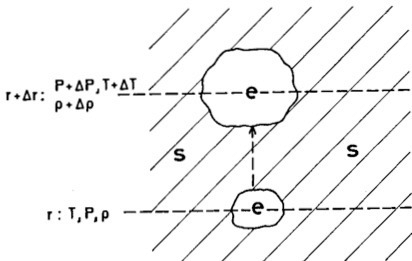
\includegraphics[width=(0.6\textwidth),height=(\textheight-11mm),keepaspectratio]{esconv}
\caption{Test of stability of a layer.}
\end{figure}

We suppose that the moving elements have no time to exchange appreciable amlount of heat with the surroundings: adiabatic movement (Dynamical instability).

Difference between the element and surroundings
\begin{equation*}
DA=A_e-A_s
\end{equation*}

\begin{itemize*}
\item For $DP\neq0$ expansion/contraction occurs at sound speed: much more rapid than other motions of elements.

We can suppose $DP=0$.

\item Let's suppose an initial fluctuation in T, $DT>0$: $DT>0$ requires that, for ideal gas ($\rho\propto\frac{P}{T}$), $D\rho<0$: the element is lighter than surroundings material, temperature fluctuations are accompained by radial local motion.

\item Let's suppose a radial displacement $\Delta r$
\begin{align*}
&D\rho=[(\TDy{r}{\rho})_e-(\TDy{r}{\rho})_s]\Delta r&\intertext{the terms in squares are change in density of the element while rises $dr$ minus spatial gradient of the surroundings}
\end{align*}

A finite $D\rho$ gives the radial component \mblock{K_r=-gD\rho} of a buoyancy force per unit of mass (g is the gravity acceleration): if $D\rho<0$ the perturbation is increased by the $K_r>0$

\end{itemize*}

Convection instability leads to cyclic macroscopic motion but the star is still in overall hydrostatic equilibrium.

\section{Condition for stability for radial fluctiations.}

\subsection{Condition for stability: density gradient}

For a radial upward fluctiation of an element:

if $D\rho<0$ the element is lighter and $K_r>0$, the situation is unstable.

If $D\rho>0$ the $K_r<0$: the element is drawn back to its original position: the layer is stable.

\begin{align*}
&(\TDy{r}{\rho})_e-(\TDy{r}{\rho})_s>0&\intertext{$\uparrow$ is highly impractical}
\end{align*}

\subsection{Condition for stability: temperature's and mean molecular weight's gradient}

\begin{align*}
&\frac{d\rho}{\rho}=\alpha\frac{dP}{P}-\delta\frac{dT}{T}+\phi\frac{D\mu}{\mu}&\intertext{with the coefficients:}\\
&\alpha=\Dcvar{\PDly{P}{\rho}}{T,\mu},\   \delta=\Dcvar{\PDly{T}{\rho}}{P,\mu},\\ &\phi=\Dcvar{\PDly{\mu}{\rho}}{T,P}&\intertext{For ideal gas:}\\
&\rho\propto\frac{P\mu}{T},\quad \alpha=\delta=\phi=1, d\mu_e=0\\
&-(\frac{\delta}{T}\TDy{r}{T})_e+(\frac{\delta}{T}\TDy{r}{T})_s-(\frac{\phi}{\mu}\PDy{r}{\mu})_s>0&\intertext{}
\end{align*}

\subsection{Scale height of pressure}

\begin{align*}
&H_P=-\frac{dr}{d\,\ln{P}}=-P\frac{P}{r}\\
&H_P=\frac{P}{\rho g}, \quad \PDy{r}{P}=-g\rho&\intertext{$H_P$ has the dimension of a length and its value represents the characteristic scale of radial pressure variation.}\\
&\parbox{1.3cm}{Solar photosphere:}\left\{\begin{array}{c}
g=2.7 \sci{4}\,cm\,s^{-2} \\
P=6.8\cdot\sci{4}\,dyn\,cm^{-2}\\
\rho=1.8\sci{-7}\,g\,cm^{-3}\\
\end{array}\right.\\
&\Rightarrow H_P=1.4\sci{7}\,cm\\
&r=\frac{\rsun}{2}:\ \left\{\begin{array}{c}
g=1.0 \sci{5}\,cm\,s^{-2} \\
P=6.7\cdot\sci{14}\,dyn\,cm^{-2}\\
\rho=1.3\,g\,cm^{-3}\\
\end{array}\right.\\
&\Rightarrow H_P=5.2\sci{9}\,cm
\end{align*}

\subsection{Condition for stability: adiabatic Temperature gradient (\sch{}).}

Anticipo il criterio di \sch{} di \ref{ssec:schcstab}.

Abbiamo visto che piccole fluttuazioni radiali di quantit\'a di materia di uno strato sferico di una stella (per esempio spostamento vero l'alto) avvengono in equilibrio di pressione con gli strati attraversati dalla porzione di materia:

The expansion of the gas element as it rises $\Delta r$ occurs on the local dynamical timescale (with  the speed of sound) and therefore the displacement and expansion of the gas element will be very close to adiabatic.

\begin{align*}
\frac{\delta P_e}{P_e}=\gamma_{Ad}\frac{\delta \rho_e}{\rho_e}&\intertext{$\gamma_{Ad}$ is the adiabatic exponent:}\\
\gamma_{Ad}=(\TDly{\rho}{P})_{Ad}\\
\TDly{P}{\rho}>\frac{1}{\gamma_{Ad}}&\intertext{$\uparrow$ criterion for stability against convection: the density gradient must be steeper than a critical value determined by $\gamma_{Ad}$}
\end{align*}

\begin{figure}[!ht]
\centering
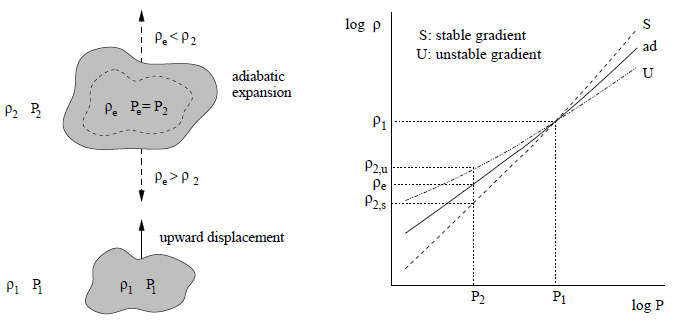
\includegraphics[width=(\textwidth),height=(\textheight-11mm),keepaspectratio]{acvsadTgrad}
\caption{A layer is stable against convection if the density varies more steeply with pressure than for an adiabatic change.}
\end{figure}

\clearpage

\section{Condiction for stability against convection: Ledoux, Schwarzschild criteria}

The following criteria to test the stability of layers against convection are local ones: easily evaluated at given place given local $P$, $T$, $\rho$ only.
\index{Local criteria for convection stability}
In extreme cases the local forces must be coupled to the neighbouring layers by momentum transfer, inertia continuity equation.

\subsection{General condition for stability: use of pressure scale height}

\begin{align*}
H_P[-(\frac{\delta}{T}\TDy{r}{T})_e+(\frac{\delta}{T}\TDy{r}{T})_s-(\frac{\phi}{\mu}\TDy{r}{\mu})_s]>0
\end{align*}

\subsection{Ledoux's criterion}

Riscrivo il criterio di stabilit\'a per fluttuazioni radiali in forma simbolica

\begin{align*}
&\underbrace{(\TDly{P}{T})_s}_{\nabla}<\underbrace{(\TDly{P}{T})_e}_{\nabla_e}+\frac{\phi}{\delta}\underbrace{(\TDly{P}{\mu})_s}_{\nabla_{\mu}}&\intertext{$()_s$ are both spatial derivatives in which P is taken as a measure of depth, $\nabla_e$ is the variation of T in the element during the motion (position is measured by P).}\\
&\nablaTact<\nel+\frac{\phi}{\delta}\nmu
\end{align*}

In a layer that transport all energy by radiation $\nablaTact=\nrad$, let's test such a layer for stability. We have supposed adiabatic change for the element fluctuations $\nel=\nad$.
We have the Ledoux criterion for stability of a radiative layer against convection (dynamical stability)

\begin{align*}
\nrad<\nad+\frac{\phi}{\delta}\nmu
\end{align*}

$\nmu\neq0$ in interior of evolving stars where heavier elements are usually produced below the lighter ones: molecular weight increases inward and the relative terms in the stability condition has a stabilizing effect ($\delta$, $\phi$ are positive).

\subsection{Schwarzschild's criterion}\label{ssec:schcstab}

In regions with homegenous chemical composition $\nmu=0$.
We have the Schwarzschild criterion for the stability of a radiative layer

\begin{align*}
\nrad<\nad
\end{align*}

\subsection{Causes of instability}

According to Schwarzschild criterion convection occurs when $\nrad=\frac{3}{16\pi acG}\frac{P}{T^4}\frac{\kappa l}{m}>\nad$.

Zones where we may found convective instability
\begin{itemize*}

\item Opaque region of stars: large value of $\kappa$. For example in outer regions of the Sun because opacity increses with decreasing temperature. Since low mass stars are cooler than high mass stars we may expect the former to have convective envelopes.

\item Regions with a large value of $\frac{l}{m}$ are regions with large energy flux. Toward the center of a star $\frac{l}{m}\approx\epsilon_{nuc}$: stars with nuclear energy production strongly peaked toward the center can be expected to have a convective core. That is the case of massive stars. 

\item We can have small values of $\nad$ in the zones of partial ionization of H and He at relatively low temperature and, even if the opacity is small the surface layers of stars may be unstable against convection. Stars of all masses have  shallow surface  convection zones at temperatures where lighter elements are partially ionized.

\end{itemize*}

\subsection{Convective zones in $\msun$ and $4\msun$ stellar model.}

\begin{figure}[!ht]
\centering
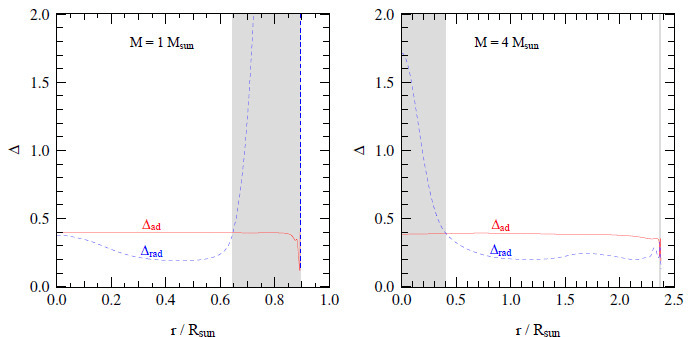
\includegraphics[width=(0.9\linewidth),keepaspectratio]{shallowconv}
\caption{Variation of $\nad$ and $\nrad$ with radius in two models at the start of main sequence.}
\end{figure}

In both models $\nad\approx0.4$ since conditions are close to an ideal gas, in the surface ionization zones $\nad<0.4$ and a thin convective layer appears in the $4\msun$ model.

The solar mass model has a very large opacity in its outer layer, resulting in a large value of $\nrad$ which gives rise to convective envelope where $\nrad>\nad$ (gray shading).

The $4\msun$ model has a hotter outer envelope with lower opacity so that $\nrad$ stay small; the large energy generation rate in the center result in a convective core.

\clearpage

\subsection{Sketch of temperature gradients}

For an unstable layer violating the \sch{} criterion we can plot the different gradients: in a $\ln{P}-\ln{T}$ diagram an adiabatic change follows a line with slope $\nad{}$, the changes in a rising element are given by $\nel{}$, while the stratifications in the surroundings and in a radiative layer are shown by lines with slopes $\nablaTact{}$ and $\nrad{}$ respectively.

Suppose $\nmu{}=0$ it follows from the violation of genaral condition for dynamic stability in the general case

\begin{equation*}
\nablaTact<\nel+\frac{\phi}{\delta}\nmu
\end{equation*}
that is $\nablaTact{}>\nel{}$. If some part of the flux is carried by convection then $\nablaTact{}<\nrad{}$ (that is to say if the entiere energy flux would be transported by radiation the actual T gradient would be greater).

Let's consider a rising element starting from $(P_0,T_0)$: this element moves downward to the left corner along the line with slope  $\nel{}$. Since $\nablaTact{}>\nel{}$, the element, although cooling, will have an increasing temperature excess over its new surroundings: it will radiates energy into its surroundings which means that the element cools more than adiabatically: $\nel{}>\nad{}$.\index{"Super-adiabatic" cooling}

\begin{align*}
\nrad{}>\nablaTact{}>\nel{}>\nad{}&\intertext{The fact that element's temperature gradient must always be between adiabatic and surroundings temperature gradients shows that the Ledoux and \sch{} criteria are also to be used in near-surface regions where the rising elements lose much of their energy by radiation:}\\
\nrad{}<\nel{}<\nad{}&\intertext{$\uparrow$ for a convective stable layer where $\nel{}>\nad{}$.}
\end{align*}

\begin{figure}[!ht]
\centering
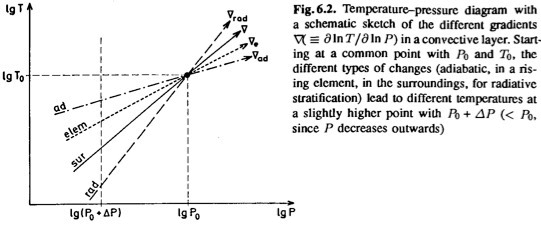
\includegraphics[width=(\textwidth),height=(\textheight-11mm),keepaspectratio]{Tgrads}
\caption{Temperature-pressure diagram with a schematic sketch of the different gradients in convective unstable layer.}
\end{figure}

\clearpage


\section{Oscillation of displaced elements}

\subsection{Equation of motion for mass elements in dynamically stable layers}

In a dynamically stable layer mass elements can oscillate around the equilibrium position because of fluctuations. Consider $\Delta r>0$

\begin{align*}
&D\rho=\frac{\rho\delta}{H_P}[\nel{}-\nablaTact{+\frac{\phi}{\delta}}\nmu{}]\Delta r&\intertext{$\uparrow$ excess of density. Remembering:}\\
&\delta=-(\PDly{T}{\rho}),\ \phi=-(\PDly{\mu}{\rho}),\\ &H_P=-\frac{dr}{d\ln{P}}=-P\TDy{P}{r}\\
&\nablaTact{}=\nablaTacte{},\ \nel{}=\nele{},\\
&\nmu{}=\nmue{}
\end{align*}

In presence of gravity acceleration g the buoyancy force per unit volume is
\begin{align*}
&K_r=-gD\rho&\intertext{producing an acceleration of the element}\\
&\PtwoDy{t}{\Delta r}=-\frac{g\delta}{H_P}[\nel{}-\nablaTact{}+\frac{\phi}{\delta}\nmu{}]\Delta r&\intertext{the righthand side is negative since in a stable layer $\frac{D\rho}{\Delta r}>0$ and thge solution of the equation of motion is of the form}\\
&\Delta r=\Delta r_0\exp{i\omega t}&\intertext{$\uparrow$ oscillations around equilibrium position.}
\end{align*}

\subsection{Frequency of oscillations: the Brunt-V\"ais\"al\"a frequency.}

The frequency of this adiabatic oscillation is the Brunt-\vai{} frequency
\begin{align*}
&\omega^2_{Ad}=\frac{g\delta}{H_P}(\nad{}-\nablaTact{}+\frac{\phi}{\delta}\nmu{})&\intertext{in unstable layers $\omega^2<0$.}
\end{align*}

\subsection{Radiative correction.}\label{ssec:radlosscil}

Suppose $DT>0$, superpose to radial energy flux $\vec{F}$, carrying energy from stellar interior to the surface, there will be a local non-radial flux $\vec{f}$, carrying the surplus energy of the element to its surroundings: the radiative flux from the elements due to its temperature excess will be

\begin{align*}
&f=\frac{4acT^3}{3\kappa\rho}|\PDy{n}{T}|&\intertext{$\PDof{n}$ is differenziation perpendicular to the surface of the element:}\\
&\PDy{n}{T}\approx\frac{2DT}{d}\\
&\lambda=Sf=\frac{8acT^3}{3\kappa\rho}DT\frac{S}{d}&\intertext{$\uparrow$ radiative loss per unit of time from the surface S of the blob, it determines the rate by which the thermal energy of the blob of volume V changes:}\\
&-\lambda=\rho Vc_P\PDy{t}{T_e}\approx\rho Vc_P\PDy{t}{DT}\\
&\PDof{t}(DT)=-\frac{DT}{\tau_{Adj}}&\intertext{$\uparrow$ ho introdotto il tempo caratteristico $\tau_{Adj}$ che \'e approx l'eccesso di calore diviso la luminosit\'a:}\\
&\tau_{Adj}=\frac{\rho Vc_P DT}{\lambda}=\frac{\kappa\rho^2c_Pd^2}{16acT^3}&\intertext{for large elements far from regions of marginal stability:}\\
&\tau_{Adj}\gg\frac{1}{\omega_{Ad}}
\end{align*}

Radiative loss gives a small deviation from adiabatic oscillations.

\section{Mixing length theory}

\subsection{Convective equilibrium}

Let's consider a layer in which the stability condition ($\downarrow$) is not fulfilled
\begin{align*}
&-\frac{1}{\gamma}\frac{1}{P}\TDy{r}{P}<-\frac{1}{\rho}\TDy{r}{\rho}\\
&-(1-\frac{1}{\gamma})\frac{T}{P}\TDy{r}{P}>-\TDy{r}{T}
\end{align*}

Hence upon the slightest perturbation convective motions will break out throughout the unstable layer: a perturbed element which is displaced upwards will have an internal density lower than the surrounding density, it experiences a net upwards force and will continues its upward motion. Similarly for an element displaced downwards.
Both downward and upward moving elements contribute to a convective energy transport upwards.

Assume initially that the layer is in precarious radiative equilibrium with the radiative flux carrying out the energy produced by nuclear processes.

Now because of instability convective motion break out throughout the layer: convective motions will transport thermal energy from lower levels to upper levels of the layer. Thus the temperature gradient will be reduced by convection and thus will be reduced the radiation flux according to equation for radiative equilibrium and the thus will be reduced also the convective energy flux since a reduction of the excess of the actual temperature gradient over the adiabatic temperature gradient.

The lowering of temperature gradient by convection will continue until the radiation flux and convective flux together fulfill the basic thermal equilibrium condition
\begin{equation*}
\TDy{r}{l(r)}=\epsilon\rho4\pi r^2
\end{equation*}

Thus instability of radiative equilibrium of a layer of a star leads to the state of convective equilibrium.

\subsection{Local flux of energy}

In an unstable layer the total flux is 

\begin{align*}
&F_{Rad}+F_{Con}=\frac{l}{4\pi r^2}=\frac{4acG}{3}\frac{T^4m}{\kappa Pr^2}\nrad{}\\
&F_{Rad}=\frac{4acG}{3}\frac{T^4m(r)}{\kappa Pr^2}\nabla_?&\intertext{part of the flux is transported by convection: $\nabla_?>\nablaTact{}$. I want to deriva an expression for}\\
&F_{Con}=\ldots\downarrow
\end{align*}

\subsection{Mean free path of mass elements: mixing length. Uncertainty.}

The mean free path of mass elements is the mixing length $l_m$ after which they dissolve in surroundings.

Great uncertainty: value of mixing length appropriates for stars. 

In Lab. mixing length is approx the linear size of volume in which convection is observed.

We may suppose the mixing length for stars to be of the order of depth of the convective layer: this could be a gross overestimate for layers in which the density drops by a large factor crossing the layer as is the case when convective instability occurs close to surface.

Uncertainty in mixing length has little consequence for convective zones in deep interior of stars, but introduce noticeable uncertainty when the convective instability occurs just below the photosphere.

\subsection{Excess thermal energy per unit volume. Relation between convective energy transport and temperature gradient.}\label{ssec:convEnT}

Let's determine the temperature excess of a rising element over its surroundings.

\begin{align*}
\delta T=(1-\frac{1}{\gamma})\frac{T}{P}\TDy{r}{P}\,dr-\TDy{r}{T}\,dr=\delta\nabla T\,dr&\intertext{$\uparrow$ difference between the adiabatic temperature change within the element and the actual temperature change in the surroundings, $\delta\nabla T$ is defined as the absolute value of the excess of actual temperature gradient  over the adiabatic temperature gradient. For the relation between $dT$ and $dP$ we use the equation of state for ideal gas and the relation between $P$ and $\rho$ for adiabatic changes.}
\end{align*}

Multiplying the temperature excess for $c_P\rho$ I have the excess of thermal energy per unit volume ($cm^3$):
\begin{align*}
&dq=c_P\,dT-\frac{\delta}{\rho}\,dP&\intertext{we will have a finite $\delta T$ while $dP$ will remain infinitesimal infinitesimal:}\\
&\delta q=c_P\rho\delta\nabla T&\intertext{where $\rho$ convert from unit of mass to unit of volume.}\\
&H=\delta\nabla T\,dr\,c_p\rho v&\intertext{$\uparrow$ Energy flux per $cm^2$ per sec}
\end{align*}

\subsection{Local convective energy flux}

Let's consider a convective element with $DT>0$ 
\begin{align*}
&F_{Con}=\rho vc_PDT&\intertext{$\uparrow$ local flux of energy:  analog to H of previous \ref{ssec:convEnT} ($dr\to\overline{dr}=\frac{l_m}{2}$). I have to consider $vDT$ as the proper mean over the whole concentric sphere.}
\end{align*}

\subsection{Radial buoyancy force. Determination of element mean velocity}\label{ssec:bmeanvelocity}

In our(\sch{}) notation $dr$ stands for average displacement (vertical distance from level at which the element had the same temperature as the surroundings): same equations hold for downward displacement $dr<0$ ($v<0$). $v$ is taken to be overall vertical velocity of all elements at one level.


I have to determine v from dynamical consideration
\begin{align*}
&\delta \rho=-\frac{1}{\gamma}\frac{\rho}{P}\TDy{r}{P}\,dr+\TDy{r}{\rho}\,dr&\intertext{$\uparrow$ deficiency of density}\\
&\delta\rho g(r)=&\intertext{$\uparrow$ excess force upward,  deficiency in gravitational force.}
\end{align*}

In more explicit form (with confusing notation $DT\leftrightarrow\delta T$): the elements passing the sphere of radius r will have different $v$ (and $DT$) and the perturbation started with $DT_0\approx0$ and $v_0\approx0$,we assume that the average element has moved $\frac{l_m}{2}$.
I average $vDT$ on the entire sphere of radius $r$.

\begin{align*}
&\frac{DT}{T}=\frac{1}{T}\PDy{r}{(DT)}\frac{l_m}{2}=(\nablaTact{}-\nel{})\frac{l_m}{2}\frac{1}{H_P}\\
&\frac{D\rho}{\rho}=-\delta(\frac{DT}{T})&\intertext{$\uparrow$ is the density difference between element and surroundings and derives from the equation of state}\\
&\frac{d\rho}{\rho}=\alpha\frac{dP}{P}-\delta\frac{dT}{T}+\phi\frac{d\mu}{\mu},\  DP=0=Du&\intertext{with}\\
&\delta=-\Dcvar{\PDly{T}{\rho}}{P}=\frac{T}{v}\Dcvar{\PDy{T}{v}}{P}\\
&K_r=-g\frac{D\rho}{\rho}&\intertext{$\uparrow$ radial buoyancy force per unit mass.}
\end{align*}

I will determine the work done by the excess force on the element: is this work which produces the kinetic energy of the element. Taking the linear approximation I have that the work done over the path between $r$ and $r+\,dr$ (integral of force excess over the path), and putting $\overline{dr}=\frac{l_m}{2}$, is 
\begin{align*}
&\frac{1}{2}K_r\frac{l_m}{2}=g\delta(\nablaTact{}-\nel{})\frac{l_m^2}{8H_P}&\intertext{Let's suppose one-half of this work $\uparrow$ goes into kinetic energy of the element $\frac{v^2}{2}$ (per unit mass) and the other half is transferred which have to be pushed aside:}\\
&v^2=g\delta(\nablaTact{}-\nel{})\frac{l_m^2}{8H_P}&\intertext{$\uparrow$ gives convection velocity as a function of temperature gradient. Holds for up/down-ward displacement since is quadratic in $dr$ and $v$.}
\end{align*}

\subsection{Changes in temperature within convective motion of velocity $v$.}

Expression for the average convective flux $F_{con}$:
\begin{align*}
&F_{Con}=\rho c_PT\sqrt{g\delta}\frac{l_m^2}{4\sqrt{2}}H_P^{-\frac{3}{2}}(\nablaTact{}-\nel{})^{\frac{3}{2}}\\
&\propto c_P\rho(\frac{Gm(r)}{Tr^2})^{\frac{1}{2}}(\delta\nabla T)^{\frac{3}{2}}\frac{l^2}{4}&\intertext{$\delta\nabla T$ represents the excess of the actual temperature gradient in absolute amount over the adiabatic temperature gradient.}
\end{align*}

Let's consider the temperature changes of a convective element with its motion with an instant velocity $v$:
\begin{align*}
&(\TDy{r}{T})_e=(\TDy{r}{T})_{Ad}-\frac{\lambda}{\rho Vc_PvT}&\intertext{$\uparrow$ the temperature change has two causes: adiabatic compression/expansion and radiative exchange of energy with the surroundings. Multiplying $\uparrow$ by $\frac{H_P}{T}$ we have:}\\
&\nel{}-\nad{}=\frac{\lambda H_P}{\rho Vc_PvT}&\intertext{$\uparrow$ $\lambda$ can be replaced by the expression derived in \ref{ssec:radlosscil}, with the average value for $DT$ given in \ref{ssec:bmeanvelocity}: the resulting equation contains a form factor $\frac{l_mS}{Vd}$.}\\
&\frac{\nel{}-\nad{}}{\nablaTact{}-\nel{}}=\frac{6acT^3}{\kappa\rho^2c_Pl_mv}
\end{align*}


\section{Character of convection in stellar interior.}

\subsection{Convection: quick equation resume.}\label{ssec:conresume}

Since we don't know how determine $l_m$ we shall treat it as a free parameter and make plausible hypothesis for its value: heat transfer operates via the largest possible elements and they can't move much more than their own diameter before differential force destroy their identity.

We have 5 equations depending on local variables ($P$, $T$, $\rho$, $l$, $m(r)$, $c_P$, $\nad{}$, $\nrad{}$, $g$):

\begin{align*}
&F_{Rad}+F_{Con}=\frac{4acG}{3}\frac{T^4m(r)}{\kappa Pr^2}\nrad{}\\
&F_{Rad}=\frac{4acG}{3}\frac{T^4m(r)}{\kappa Pr^2}\nablaTact{}\\
&v^2=g\delta(\nablaTact{}-\nel{})\frac{l_m^2}{8H_P}\\
&F_{Con}=\rho c_PT\sqrt{g\delta}\frac{l_m^2}{4\sqrt{2}}H_P^{-\frac{3}{2}}(\nablaTact{}-\nel{})^{\frac{3}{2}}\\
&\frac{\nel{}-\nad{}}{\nablaTact{}-\nel{}}=\frac{6acT^3}{\kappa\rho^2c_Pl_mv}&\intertext{$\uparrow$ adiabatic approximation: ignore radiative correction.}
\end{align*}
and we can solve for $F_{Rad}$, $F_{Con}$, $v$, $\nel{}$, $\nablaTact{}$.

\subsection{Euristic justification of adiabatic approximation in stellar interior.}

The solution of the complete equations for actual temperature gradient can be simplified since for convective layers in stellar interior $\nablaTact{}\approx\nad{}$:
\begin{align*}
\TDy{r}{T}\to(1-\frac{1}{\gamma})\frac{T}{P}\TDy{r}{P}&\intertext{we insert $\uparrow$ in the set of equations of \ref{ssec:conresume}}\\
\nad{}\approx\nel{}\approx\nablaTact{}
\end{align*}

Numerical estimate for median point in the sun (and $F_{Con}$'s upper limit):
\begin{align*}
(\Delta\nabla T)\approx2\sci{-10},\quad |\TDy{r}{T}|\approx\frac{T_c}{R}\approx3\sci{-4}&\intertext{the excess of temperature gradient over adiabatic temperature gradient is $\sci{-6}$ of temperature gradient itself.}
\end{align*}

When we approach the photosphere density and mixing length are much smaller than in stellar interior and we have to solve full set of convective equations explicitly (see \ref{ssec:conresume}).

\subsection{Chaotic convective motions.}

For a median point in the sun the average temperature excess/deficiency within moving element respect to surroundings is $\overline{\delta T}=\Delta\nabla T\overline{dr}\approx1\,K$: that is a small fluctuation compared to a temperature of several millions K.

We can estimate the convective velocity typical for the sun to be $v_c\approx0.03 Km/s$, small compared to typical thermal velocities of stellar interior $v_{th}\approx10^2\,Km/s$.

Since convective velocities are smaller than thermal velocities by about 4 power of ten the hydrodynamic effects of the convective motions must be smaller than the gas pressure force by about 8 power of ten:

this circumstance justifies our tacit assumption that the convective motions don't disturb hydrostatic equilibrium.

The Raynold number (computed from convective velocity) is much larger than critical value (consequence of large linear scale): convection will not occur in orderly semi-stable patterns, such in Benard cells, but rather in a chaotic turbolent manner.

Average lifetime of a turbolent element is $t\approx\frac{l_m}{v}\approx2\sci{6}\,s\approx20\,d$: convective layers are mixed very efficiently. When nuclear transmutation changes the composition of the hottest parts of convective layers changes become apparent in the whole layers.

Motion in convective layers:
\begin{itemize*}
\item Turbolent.
\item So slow that doesn't have hydrodynamic effects.
\item Highly efficient in transporting energy because of high content of thermal energy of gasses in stellar interior.
\item Turbolent mixing is so fast that a convective region is practically homogemeous in composition.
\end{itemize*}

\subsection{Convective mixing}

La convezione trasporta efficientemente energia e riduce le differenze di composizione chimica

\begin{align*}
&l_m\approx H_P\\
&\sqrt{gH_P}\approx v_s,\ v_s\approx\sqrt{\frac{GM}{R}}\\
&v_c\approx v_s\sqrt{gH_P}&\intertext{typically convective velocity are strongly subsonic \num{e-3} except in outer layers.}\\
&\nabla-\nad{}\approx(\frac{LR}{M})\expy{\frac{2}{3}}\frac{R}{GM}\\
&v_c\approx(\frac{LR}{M})\expy{\frac{1}{3}}\approx\SI{5e3}{\cm\per\second}\\
&d=qR,\ \tau_{Mix}\approx\frac{d}{v_c}\approx q\SI{e7}{\second}
\end{align*}


\subsection{Dimensionless equation for actual gradient.}

Nel caso la luminosit\'a sia trasportata esclusivamente dalla radiazione il gradiente di temperatura \'e dato da
\begin{align*}
&\nrad{}=\Dcvar{\TDly{P}{T}}{Rad}\\
&=\frac{3}{16\pi acG}\frac{\kappa l(r)P}{mT^4}
\end{align*}

Quando il trasporto di energia avviene anche per convezione il gradiente di temperatura \'e $\nabla<\nrad{}$; il flusso totale \'e
\begin{equation*}
\frac{l(r)}{4\pi r^2}F_{Conv}+F_{Rad}=\frac{4acG}{3}\frac{T^4m}{\kappa Pr^2}\nrad{}
\end{equation*}

e per $F_{Rad}$ ho (vedi equilibrio radiativo)

\begin{equation*}
F_{Rad}=\frac{4acG}{3}\frac{T^4m}{\kappa Pr^2}\nabla
\end{equation*}

Per il flusso convettivo ho, supponendo che il moto della bolla di gas  con velocit\'a v sia in equilibrio di pressione con l'ambiente $DP=0$, abbiamo
\begin{align*}
F_{Conv}=\rho v c_PDT&\intertext{$DT$ \'e la differenza di temperatura rispetto all'ambiente.}
\end{align*}

Riduco il sistema introdotto in (\ref{ssec:conresume}) ad una equazione adimensionale da cui ricavo il gradiente di temperatura.

Introduco le quantit\'a adimensionali
\begin{align*}
&U=\frac{3acT^3}{c_P\rho^2\kappa l_m^2}\sqrt{\frac{8H_P}{g\delta}}\\
&W=\nrad{}-\nad{}
\end{align*}
entrambe sono calcolabili data la struttura stellare e $l_m$.

Ottengo cos\'i un sistema di 2 equazioni
\begin{align*}
&\nabla_e-\nad{}=2U\sqrt{\nabla-\nabla_e}\\
&(\nabla-\nabla_e)\expy{\frac{3}{2}}=\frac{8}{9}U(\nrad{}-\nabla)
\end{align*}

infine, definendo $\xi^2=\nabla-\nad{}+U^2$ di cui considero la radice positiva, ottengo un'equazione cubica per $\xi$ risolvibile per dati U,W
\begin{equation*}
(\xi-U)^3+\frac{8U}{9}(\xi^2-U^2-W)=0
\end{equation*}

L'equazione sopra ha una sola soluzione reale che tramite la $\xi$ fornisce il gradiente di temperatura media $\nabla$ che si stabilisce in strati convettivi.


\subsection{Casi limite: convection in very dense central part and near photosphere.}

For a given $W=\nrad{}-\nad{}$ the convection depends on U:
\begin{align*}
&F_{Rad}=\sigma_{Rad}\nabla\\
&F_{Con}=\sigma_{Con}(\nabla-\nabla_e)\expy{\frac{3}{2}}&\intertext{U is essentially the ratio of conductivities}\\
&U\approx \frac{\sigma_{Rad}}{\sigma_{Con}}&\intertext{and can also be written in terms of $\tau_{ff}$ the time it takes a mas element to fall freely over the distance $H_P$}\\
&U\approx\frac{\tau_{ff}}{\tau_{adj}}\frac{d^2}{l_m}&\intertext{d is the linear dimension of the blob,}\\
&\tau_{ff}=\sqrt{\frac{2H_P}{g}},\  \tau_{Adj}=\frac{\kappa\rho^2c_Pd^2}{16acT^3}\frac{\rho Vc_PDT}{\lambda}&\intertext{, characteristic time for thermal adjustment caused by $DT=T_e-T_s$, $\lambda$ is the radiative loss. Normally $d\approx l_m$ and therefore}\\
&U\approx\frac{\tau_{ff}}{\tau_{Adj}}
\end{align*}

Definisco la quantit\'a adimensionale
\begin{equation*}
\Gamma=\frac{\sqrt{\nabla-\nabla_e}}{2U}=\frac{\nabla-\nabla_e}{\nabla_e-\nad{}}
\end{equation*}

for a roughly spherical element of radius $\frac{l_m}{2}$, cross section A, volume V, lifetime $\tau_l=\frac{l_m}{v}$, thermal energy $e_{th}=\rho Vc_PT$, one finds
\begin{align*}
&\nabla-\nabla_e=\frac{(F_{Con}A)\tau_l}{e_{th}}\frac{4H_P}{3l_m}&\intertext{using equations for $\frac{DT}{T},\ F_{Con}$ from \ref{ssec:bmeanvelocity}, and}\\
&\nabla_e-\nad{}=\frac{\lambda\tau_l}{e_{th}}\frac{H_P}{l_m}
\end{align*}

quindi, $\Gamma$ \'e il flusso di energia attraverso la superficie A per secondo relativo all'energia irradiata dall'elemento

\begin{equation*}
\Gamma\approx\frac{AF_{Con}}{\lambda}=\frac{\text{Energy transported}}{\text{Energy lost}}
\end{equation*}

Fatti:
\begin{itemize}
\item $\Gamma$ is a measure for efficiency of convection: large values of $\Gamma$ (small of U) are typical for very dense matter where radiation losses are relatively unimportant compared to convective flux. 
\item In regions of low density radiative losses can be large and convection ineffective for energy transport; the elements lose all of their excess heat through radiation to surroundings: $DT\approx0$. In this case $\Gamma$ small (U large).
\item The meaning of $\Gamma$ can also be represented in terms of lifetime and adjustment time
\begin{equation*}
\Gamma=\frac{\nabla-\nabla_e}{\nabla_e-\nad{}}=2\frac{\tau_{Adj}}{\tau_{l}}
\end{equation*}
\end{itemize}

Casi limite:
\begin{itemize}
\item $U\to0\ (\Gamma\to\infty)$: $\nabla_e\to\nad{}$ and $\nabla\to\nad{}$. This is the case of very dense central part of a star.

\item $U\to\infty\ (\Gamma\to0)$: $\nabla\to\nrad{}$ therefore $F\to F_{Rad}$. This is the case near the photosphere of a star.

\end{itemize}

Where the limiting case do not apply the equations of the mixing length theory yield a value for $\nabla$ somewhere between $[\nad{},\nrad{}]$, the convection being said to be superadiabatic.



\part{Stato della materia, equazione di stato, ionizzazione, (produzione di energia, opacit\'a)}
\chapter{Photon diffusion approximation} \label{chap:stellarinterior}
\PartialToc



\section{Equazione di stato}

\subsection{Legge dei gas perfetti e stato di ionizzazione della materia stellare}

Nell'interno stellare si raggiunge rapidamente l'equlibrio su scala atomica ma non nucleare (steady macroscopic state: principles of statistical physics): rates of all atomic reactions equal those of their reverse.

Le funzioni che descrivono uno stato di equilibrio dipendono dalla composizione chimica (:$\mu$), $\rho$, T.

Una funzione $P=P(\rho,T)$ \'e la funzione di stato: struttural support against gravity.

Vicino alla superficie la funzione di stato \'e complicata dalla presenza di atomi parzialmente ionizzati.

Per $T\geq 10^5 K$ diventa viavia pi\'u esatto considerare il gas completamente ionizzato; the bulk of the structure of most stars is detemined by an equation of state for completely ionized matter. Completely ionized gas behave like perfect gas up to high densities: radii of nuclei are $10^{-5}$ those of atoms, a gas composed of nuclei and electrons occupies $\approx10^{-15}$ of the volume occupied by atoms.

In un gas perfetto le interazioni fra particelle sono trascurabili $E_{int}\approx\exv{E_{Cou}}\ll KT$ for non degenerate gas.


\begin{align*}
&n=\frac{N}{V}\\
&\rho=\frac{M}{V}\\
&m_0=\frac{M}{N}&\intertext{\'e il peso molecolare medio}\\
\end{align*}
ho l'equazione di stato
\begin{align*}
&PV=nRT=NKT&\intertext{Riscrivo l'equazione di stato esprimendo la pressione in funzione della densit\'a, temperatura e composizione}\\
&P=(\frac{N}{V})KT=nKT=\frac{\rho}{m_0}KT\\
&P=\frac{1}{\mu}\frac{K_B}{m_P}\rho T&\intertext{definisco il peso molecolare in termini di proton mass}\\
&\frac{1}{\mu}=2X+\frac{3}{4}Y+\frac{Z}{2}
\end{align*}

\begin{usefull}{Peso molecolare medio}

Equazione di stato per un gas di particelle materiali non-interacting non-degenerate

\begin{align*}
&P_g=nkT\\
&P_g=(\frac{\gasconstant{}}{\mu})\rho T&\intertext{dove $\gasconstant{}$ \'e in moli $\mu$ \'e il peso molecolare medio (massa per mole di particelle libere)}
\end{align*}

\begin{definition}{Peso molecolare medio}
Segue dalla definizione di mole che $\mu$, the total rest mass per mole of free particles is also equal to average rest mass in amu per free particles ($\si{\atomicmassunit}=\frac{1}{N_A}\approx M(H^1)$): $\mu$ depends on number of free particles contained in a fixed rest mass of the material (fixed value of the product of the number of free particles in the system and average rest mass per free particle).

\begin{align*}
&\mu=(\frac{\rho}{H})\frac{1}{n}=\frac{\sum_kA_kn_k}{\sum_kn_k}&\intertext{where}\\
&A_k=\frac{m_k}{H},\ n_k=\frac{\rho x_k}{HA_k}\\
&\mu=\frac{1}{\sum_k\frac{x_k}{A_k}}
\end{align*}

In case free electrons have been released by ionization of atoms
\begin{align*}
&n=n_e+\sum_in_i&\intertext{$n_e$ is the number density of ionization electrons. Sia $\nu_e(i)$ il numero medio di elettroni liberati da ionizzazione specie i:}\\
&n_e=\sum_i\nu_e(i)n_i=\frac{\rho}{H}\sum_i\nu_e(i)\frac{x_i}{A_i}\\
&n=\frac{\rho}{H}\sum_i[1+\nu_e(i)]\frac{x_i}{A_i}=\frac{\rho}{H}\sum_i\bar{n}_ix_i&\intertext{where $\frac{[1+\nu_e(i)]}{A_i}$ is what Chandra called ''mean ionization per unit atomic weight'': total number of free particle per unit atomic mass contributed by particles of type i and atomic weight $A_i$.}\\
&\bar{n}_H=\frac{2}{1.008}\approx2,\ \bar{n}_{He}=\frac{3}{4.004}\approx0.75\\
&\mu=\frac{1}{\sum_i\bar{n}_ix_i}&\intertext{Assuming heavier elements than He completely ionized (and $A_i\approx2Z_i$ so that $\bar{n}_i\approx\frac{1}{2}$ for ($Z_i>2$)):}\\
&\mu=\frac{1}{\bar{n}_HX+\bar{n}_{He}Y+\bar{n}_{Z}Z}\\
&\mu\approx\frac{1}{2X+\frac{3}{4}Y+\frac{1}{2}Z}&\intu{for complete ionization}
\end{align*}

\end{definition}

The process of ionization dissociation and nuclear reaction alter the number of free particles in a given mass of the gas.


\end{usefull}


\subsection{Composizione chimica: numero di particelle libere per unit\'a di volume e peso molecolare medio $\mu$}
\index{Peso molecolare: particelle libere. ???}
We want to relate number of free particles N to the density; ho le lettere standard per l'abbondanza degli elementi: $X+Y+Z=1$ e A peso atomico medio per elementi pi\'u pesanti dell'elio

\begin{tabular}{c|ccc}
Elements: & $^1H$ & $^4He$ & Heavier\\
\hline
 $\#$ atoms per $cm^3$ & $\frac{X\rho}{m_p}$ & $\frac{Y\rho}{4m_p}$ & $[\frac{Z\rho}{Am_p}]$\\
 $\#$ electrons per $cm^3$ & $\frac{X\rho}{m_p}$ & $\frac{2Y\rho}{4m_p}$ & $\frac{1}{2}A\frac{Z\rho}{Am_p}$
\end{tabular}

In a completely ionized gas the number of free particles per cubic centimeter is 
\begin{equation*}
N=(2X+\frac{3}{4}Y+\frac{1}{2}Z)\frac{\rho}{m_p}
\end{equation*}

L'equazione di stato dei gas perfetti diventa
\begin{align*}
P=\frac{1}{\mu}\frac{K_b}{m_p}\rho T\\
\frac{1}{\mu}=2X+\frac{3}{4}Y+\frac{1}{2}Z
\end{align*}

Definizioni alternative di peso molecolare medio

\begin{align*}
&\rho=n\mu m_u&\intertext{n particelle per unit\'a di volume con stesso peso molecolare $\uparrow$. In generale}\\
&n_i=\frac{\rho_i}{\mu_im_u}=\frac{\rho}{m_u}\frac{X_i}{\mu_i}&\intertext{e per atomi completamente ionizzati (nucleus + free electrons)}\\
&n=n_e+\sum_in_i=\sum_i(1+Z_i)n_i\tikzmark{first}\\
&P=nkT=R\sum_i(\frac{X_i(1+Z_i)}{\mu_i})\rho T\tikzmark{second}
\end{align*}


Atomo neutro e contributo elettroni liberi.

Per un gas composto da atomi neutri ho:

$\mu_0=(\sum_i\frac{X_i}{\mu_i})^{-1}$.

Per gas completamente ionizzati definisco il peso molecolare medio per elettroni liberi:

\begin{align*}
&\mu_e=(\sum_iX_iZ_i/\mu_i)^{-1}&\intertext{for elements heavier than helium $\frac{\mu_i}{Z_i}\approx2$}\\
&\approx(X+\frac{1}{2}Y+\frac{1}{2}(1-X-Y))^{-1}=\frac{2}{1+X}
\end{align*}


\subsection{Gas di fotoni}


In prima approssimazione in un interno stellare
\begin{align*}
&P=P_g+P_{rad}=\frac{R}{\mu}\rho T+\frac{a}{3}T^4\\
&P_{Rad}=\frac{1}{3}\int_0^{\infty}\frac{h\nu}{c}cn(\nu)\,d\nu\\
&=\frac{1}{3}U=\frac{a}{3}T^4&\intertext{$\uparrow$ \'e la densit\'a di energia e}\\
&a=7.56*10^{-15}\,erg\,cm^{-3}\,K^{-4}
\end{align*}

Misuro l'importanza della pressione di radiazione con il parametro $\beta$
\begin{align*}
&\beta=\frac{P_g}{P}\\
&1-\beta=\frac{P_{Rad}}{P}
\end{align*}
\index{Parametro beta}

\begin{definition}{Emission coefficient}
Let's consider small mass element m which is radiating: the amount of radiant energy emitted by solid angle $d\omega$, frequency interval $[\nu,\nu+d\nu]$ and time $dt$

\begin{equation*}
j_{\nu}m\,d\omega\,dt\,d\nu
\end{equation*}

$j_{\nu}$ is called emission coefficient for frequency $\nu$.

\end{definition}



\subsection{Einstein coefficient.}

\begin{definition}{Spontaneous/induced emission coefficient.}

The probability that an atom in an excited state n emits in direction $d\omega$ and time $dt$ quanta of energy $h\nu_{nm}$ in absence of sxternal field is
\begin{equation*}
    A_{nm}\,d\omega\,dt
\end{equation*}

In presence of external field of radiation of intensity $I_{\nu_{nm}}$
\begin{equation*}
B_{nm}I_{\nu_{nm}}\,d\omega\,dt
\end{equation*}

\end{definition}

\subsection{Thermodynamical equilibrium.}

\subsection{Radiative equilibrium.}

La pressione di radiazione agisce a tutti gli effetti come una pressione cio\'e il suo gradiente \'e una forza 
\begin{align*}
&[H]=\text{Net energy transport/$cm^2$/s}\\
&F_{Rad}=\kappa_{\rho}H\frac{1}{c}\\
&F_{Rad}=-\frac{d}{dr}(\frac{a}{3}T^4)=-\frac{dP_R}{dr}
\end{align*}



\section{Adiabatic processes}

Most of the gas in a star can be thought as adiabatic: any process that take place on a timescale shorter than $\tkh{}$ can be thought of as adiabatic.

\begin{align*}
&\TDy{t}{u}+P\TDof{t}\frac{1}{\rho}=\epsilon-\TDy{m}{F}=0&\intertext{and for many types of gas $u=\phi\frac{P}{\rho}$ quindi}\\
&\frac{dP}{P}=(\frac{\phi+1}{\phi})\frac{d\rho}{\rho},\ \ln{P}=\gamma_a\ln{\rho}+\ln{K_a}&\intertext{the constant $K_a$ is determined by the entropy of the gas}
\end{align*}

All monoatomic ideal gas have $\gamma_a=\frac{5}{3}$, all relativistic gasses have $\gamma_a=\frac{4}{3}$.

Nel caso $K_a$ sia costante, tipo nella zone convettive, posso usare una relazione politropica con $\gamma_P=\gamma_a$.

\begin{usefull}{Difference polytropic relation vs adiabatic exponent}

\begin{itemize}
\item Polytropic relation describes how pressure change with density inside as one moves through the star.
\item Adiabatic equation of state describe how how a given gas shell would respond to being compressed.
\end{itemize}

\end{usefull}


\section{Ionizzazione}

\subsection{Idrogeno}
Definisco il grado di ionizzazione ($x=1$ per gas completamente ionizzato, $x=0$ per gas neutro)
\begin{equation*}
x=\frac{n_1}{n_0+n_1},\quad\frac{n_1}{n_0}=\frac{x}{1-x}
\end{equation*}
\index{Grado di ionizzazione: $^1H$}

Equazione di Saha
\begin{align*}
&\frac{n_{r+1}}{n_r}P_e=\frac{xP_e}{1-x}\\
&P_e=\frac{x}{1+x}P_{Gas}\\
&\frac{x^2}{1-x^2}=K_H\\
&K_H=\frac{u_1}{u_0}\frac{2}{P_{Gas}}\frac{(2\pi m_e)^{\frac{3}{2}}}{h^3}(KT)^{\frac{5}{2}}\exp{-\frac{\chi_H}{KT}}\\
&\chi_H=13.6\, eV
\end{align*}

Nella fotosfera (cgs) \mblock{P_{Gas}=6.83*10^4,\ T=5636\,K}: $x=10^{-4}$.

Deep layer (cgs) \mblock{P_{Gas}=1.56*10^{12},\ T=7.15*10^5\,K}: $x=0.993$.

Comportamento di $K_H$ in funzione di T e $P_{Gas}$:

aumenta con T e decresce con la pressione e stessa cosa per il grado di ionizzazione. Infatti con T aumenta anche l'energia delle collisioni e dei fotoni, mentre all'aumentare di $P_{Gas}$ aumenta la probabilit\'a di ricombinazione elettroni/ioni.

Determino $\mu$ per gas di idrogeno con grado di ionizzazione x: $\mu m_u$, $\mu_0m_u$, $\mu_em_u$ sono definiti come masse medie per, rispettivamente, particelle libere,  nuclei ed elettroni liberi.

Numero di elettroni liberi per atomo: \mblock{E=\frac{n_e}{n}=x}.
\begin{align*}
\rho=(n+n_e)\mu m_u=n\mu_0m_u=n_e\mu_em_u&\intertext{Usando $n=n_0+n_1$, risolvo per $\mu$: $\downarrow$}\\
\mu=\frac{\rho}{m_un}\frac{1}{1+x}=\frac{\mu_0}{1+x}=\mu_e\frac{x}{1+x}&\intertext{$\uparrow$ \'e valida per miscela di gas salvo che $E\neq x$}
\end{align*}
\index{Mean molecular weight for partially ionized hydrogen}

\subsection{H-He mixture}

Ho un gas di idrogeno ed elio di abbondanze relative X e Y: 3 energie di ionizzazione per idrogeno neutro $\chi_H^0=13.6\,eV$ e $\chi_{He}^0=24.6\,eV$, $\chi_{He}^1=54.4\,eV$ per elio neutro e 1-ionizzato.

Contributi energia interna atomi ionizzati.
\begin{itemize*}
\item Ogni atomo di idrogeno ionizzato contribuisce $\chi_H^0$.
\item Ogni atomo di He ionizzato 1 volta contribuisce $\chi_{He}^0$
\item Ogni atomo di He privo di elettroni $\chi_{He}^0+\chi_{He}^1$
\end{itemize*}

Definisco il grado di ionizzazione $x_i^r$ (il numero di atomi di tipo i ionizzati r diviso il numero totale di atomi i):
\begin{align*}
&x_H^0=\frac{n_H^0}{n_H},\quad x_H^0=\frac{n_H^1}{n_H}\\
&x_{He}^0=\frac{n_{He}^0}{n_{He}},\quad x_{He}^1=\frac{n_{He}^1}{n_{He}},\quad x_{He}^2=\frac{n_{He}^2}{n_{He}}
\end{align*}

Contributo dell'energia di ionizzazione all'energia interna
\begin{align*}
&u_{ion}=\frac{1}{m_u}\{Xx_H^1\chi_H^0\\
&+\frac{1}{4}Y[x_{He}^1\chi_{He}^0+x_{He}^2(\chi_{He}^0+\chi_{He}^1)]\}&\intertext{$\frac{X}{m_u}$ \'e il numero di atomi d'idrogeno, $\frac{Y}{4m_u}$ \'e il numero di atomi di elio}
\end{align*}

Ho 3 equazioni di Saha: 6 equazioni per sei incognite $x_H^0$, $x_H^1$, $x_{He}^0$, $x_{He}^1$, $x_{He}^2$, $E$.

\begin{align*}
&\frac{x_H^1}{x_H^0}\frac{E}{E+1}=K_H^0\\
&\frac{x_{He}^1}{x_{He}^0}\frac{E}{E+1}=K_{He}^0\\
&\frac{x_{He}^2}{x_{He}^1}\frac{E}{E+1}=K_{He}^1&\intertext{$\uparrow$ equazioni di Saha: sono occoppiate tra loro tramite $E$. Inoltre:}\\
&E=[Xx_H^1+\frac{1}{4}Y(x_{He}^1+2x_{He}^2)]\mu_0\\
&K_i^r=\frac{u_{r+1}}{u_r}\frac{2}{P_{Gas}}\frac{(2\pi m_e)^{\frac{3}{2}}(KT)^{\frac{5}{2}}}{h^3}\exp{-\frac{\chi_i^r}{KT}}\\
&x_H^0+x_H^1=1,\quad x_{He}^0+x_{He}^1+x_{He}^2=1
\end{align*}


\chapter{Ionized real gas}
\PartialToc

\section{Grandezze termodinamiche di un plasma classico}

\subsection{Passoggio da unit\'a energetiche a gradi (Landau)}

\begin{align*}
&k=\SI{1.38e-16}{\erg\per\kelvin},\ \SI{1}{\ev}=\SI{11606}{\kelvin}\\
&S=k\ln{\Delta\Gamma}\\
&T\to kT,\ S\to\frac{S}{k}
\end{align*}

\subsection{Sviluppo in serie di potenze della  densit\'a per un gas neutro}

Considero il gas abbastanza rarefatto in modo da poter trascurare le collisioni che coinvolgono pi\'u di 2 atomi/molecole. Per un gas monoatomico reale classico l'energia si scrive \mblock{E(p,q)=\sum^N\frac{p_a^2}{2m_a}+U} e $U$ \'e l'energia di interazione tra gli atomi.

\begin{align*}
&F=-kT\ln{\int\exp{-\frac{E(p,x)}{kT}}\,d\Gamma}&\intertext{considerando anche le interazioni}\\
&F=F_{perf}\\
&-kT\ln{\frac{1}{V^N}}\int d^3p_1\ldots\,d^3p_N\int\exp{-\frac{U}{kT}}d^3x_1\ldots\,d^3x_N\\
&F=F_{perf}\\
&+\frac{N^2TB(T)}{V},\ B(T)=\frac{1}{2}\int(1-\exp{-\frac{U_{12}}{kT}})\,d^3x&\intertext{da cui trovo la pressione e quindi l'equazione di stato aanell'approssimazione considerata}\\
&P=-\PDy{V}{F}=\frac{NkT}{V}(1+\frac{NB(T)}{V})
\end{align*}

Lo sviluppo in serie di potenze di $\frac{1}{V}$ \'e
\begin{equation*}
P=\frac{NkT}{V}(1+\frac{NB(T)}{V}+\frac{N^2C(T)}{V^2}+\ldots)
\end{equation*}

B, C sono il secondo e il terzo coefficiente del viriale.

Per determinare questi coefficienti considero il potenziale
\begin{align*}
&\exp{-\frac{\Omega}{kT}}=\sumzi{N}\frac{1}{N!}\exp{\frac{\mu N}{kT}}\int \exp{-\frac{E_N(p,x)}{kT}}\,d\Gamma_N\\
&E_3(p,x)=\sum\frac{p_a^2}{2m_a}+U_{123}
\end{align*}

\subsection{Gas completamente ionizzato}

Per calcolare le correzioni di un gas di particelle interagenti tramite forza coulombiana \'e necessario sviluppare una tecnica diversa da quella dello sviluppo in termini del viriale per gas di particelle neutre.

Considero il gas completamente ionizzato e globalmente neutro: \mblock{\sum_az_aeN_{a0}}. Supponiamo che il gas devii dallo stato perfetto: \'e indispensabile che l'energia coulombiana media tra due ioni \mblock{\frac{(ze)^2}{\overline{r}}}, con \mblock{\overline{r}\approx r\expy{-\frac{1}{3}}} distanza media tra gli ioni, sia piccola rispetto all'energia cinetica $kT$:
\begin{align*}
&(ze)^2n\expy{\frac{1}{3}}\ll kT\\
&n\ll(\frac{kT}{z^2e^2})^3 
\end{align*}

Poich\'e il plasma \'e elettricamente neutro il valore medio dell'energia di interazione coulombiana tra le particelle se fossero uniformemente distribuite in maniera indipendente si annullerebbe.

\begin{definition}{Correzione correlative delle grandezze termodinamiche}

Le prime correzioni alle grandezze termodinamiche del plasma rispetto al gas perfetto compaiono se si tiene conto delle correlazioni tra le diverse particelle.

\end{definition}

Per la correzione all'energia coulombiana del plasma $E_{cor}$ scrivo l'energia di interazione elettrostatica di un sistema di particelle cariche come

\begin{equation*}
E_{cor}=V\frac{1}{2}\sum_aez_an_{a0}\phi_a
\end{equation*}

dove $\phi_a$ \'e il potenziale creato dalle altre particelle cariche e agente sullo ione dell'a-esimo tipo.

Ciascuno ione crea attorno a se una nube ionica a simmetria sferica: indicando con $n_a$ la densit\'a degli ioni dell'a-esimo tipo in questo nube ionica, l'energia potenziale di ciascuno ione dell'a-esimo tipo nel campo esistente attorno al dato ione \'e $ez_a\phi$ dove $\phi$ \'e il potenziale del campo. In accordo con la formula di Boltzmann abbiamo
\begin{equation*}
n_a=n_{a0}\expp{(-\frac{z_ae\phi}{kT})}
\end{equation*}

il coefficiente costante si \'e posto $n_{a0}$ poich\'e lontano dal centro \mblock{\phi\to0} la densit\'a della nube ionica diventa la densit\'a media del gas.

Il potenziale $\phi$ del campo elettrico nella nube ionica \'e legato alla densit\'A di cariche, \mblock{\sum ez_an_a}, dall'equazione di Poisson

\begin{equation*}
\nabla^2\phi=-4\pi e\sum_az_an_a
\end{equation*}

Le ultime due equazioni definiscono il campo elettrico autocompatibile di elettroni e ioni.

Vista l'ipotesi di piccola energia di interazione tra gli ioni posso espandere gli esponenziali al termine lineare nel campo elettrico:

\begin{align*}
&\nabla^2\phi-\kappa^2\phi=0\\
&\kappa^2=\frac{4\pi e^2}{kT}\sum_an_{0a}z_a^2
\end{align*}

$\kappa$ \'e l'inverso di una lunghezza e la soluzione a simmetria sferica dell'equazione precedente \'e 
\begin{equation*}
\phi\propto\frac{\exp{-\kappa r}}{r}\\
\phi=ez_b\frac{\exp{-\kappa r}}{r}
\end{equation*}
la costante moltiplicativa si ha considerando che il potenziaöe per piccole distanze dal centro \'e $\frac{ez_b}{r}$. Il campo diventa molto piccolo a distanze grandi rispetto a $\frac{1}{\kappa}$.

\begin{definition}{Raggio di Debye}

La lunghezza \mblock{\frac{1}{\kappa}=\sqrt{\frac{kT}{4\pi e^2\sum_zz^2\overline{n}_z}}}.

\end{definition}

L'approssimazione di interazione debole \'e equivalente alla condizione che il raggio di Debye sia molto pi\'u grande della distanza media tra gli ioni.

Sviluppando il potenziale autocompatibile
\begin{equation*}
\phi=\frac{ez_b}{r}-ez_b\kappa+\ldots
\end{equation*}
i termini omessi si annullano per $r=0$. Il primo termine \'e il campo coulombiano dello ione in esame, il secondo \'e il campo creato da tutti gli altri ioni della nube nel punto in cui si trova lo ione dato quindi
\begin{align*}
&E_{cor}=V\frac{1}{2}\sum_aez_an_{a0}\phi_a&\intertext{sostituendo $\phi_a=-ez_a\kappa$}\\
&E_{cor}=-\frac{V}{2}\kappa e^2\sum_an_{a0}z_a^2=-Ve^3\sqrt{\frac{\pi}{kT}}(\sum_an_{a0}z_a^2)\expy{\frac{3}{2}}
\end{align*}

Dalla relazione termodinamica
\begin{align*}
&E=F-T\Dcvar{\PDy{T}{F}}{V}=-T^2\Dcvar{\PDof{T}\frac{F}{T}}{V}&\intertext{e ponendo la costante di integrazione uguale a zero poich\'e \mblock{F\abc{T\to +\infty}F_{perf}}}\\
&F=F_{perf}-\frac{2e^3}{3}\sqrt{\frac{\pi}{kTV}}(\sum_aN_az_a^2)\expy{\frac{3}{2}}&\intertext{ponendo $N_a=n_{a0}V$.}
\end{align*}

e per la pressione:

\begin{align*}
&P=_\Dcvar{\PDy{V}{F}}{T}\\
&P=\frac{NkT}{V}-\frac{e^3}{3V\expy{\frac{3}{2}}}\sqrt{\frac{\pi}{kT}}(\sum_aN_az_a^2)\expy{\frac{3}{2}}
\end{align*}

\section{Real ionized gas: coulomb pressure}


In presence of forces tbhe internal energy of mono-atomic gas must include potential energy of interaction
\begin{equation*}
E_i=\sum\frac{p^2}{2m}+\Phi
\end{equation*}
where $\Phi$ is the potential energy, depends upon interparticle distance and so upon density.

\subsection{Nearly perfect gas at low density: \mblock{n_Z\ll(\frac{kT}{Z^2e^2})^3}.}

The pressure is given by change in internal energy $dE_i$ associated with adiabatic compression \mblock{\Dcvar{dE_i}{ad}=-P\,dV}: if the internal energy is density dependent because of icoulomb interaction a pressure arises.

The Coulomb energy per unit volume is
\begin{equation*}
\Dcvar{\frac{U}{V}}{c}=\frac{1}{2}\sum_ZeZ\overline{n}_Z\Phi_Z
\end{equation*}



Riscrivo il raggio di Debye utilizzando il coefficiente $\zeta$
\begin{align*}
&\sum_ZZ^2\overline{n}_Z=\sum_Z(Z^2+Z)\overline{n}_Z=\sum_Z(Z^2+Z)\frac{\rho X_Z}{A_Z}N_A\\
&R_D=\sqrt{\frac{kT}{4\pi e^2\rho N_A\xi}}&\intertext{dove ho definito}\\
&\xi=\sum_{+Z}(Z^2+Z)\frac{X_Z}{A_Z}\\
\end{align*}
da cui l'energia potenziale coulombiana per unit\'a di volume:
\begin{align*}
&\Dcvar{\frac{E_i}{V}}{c}=-e^3\sqrt{\frac{\pi}{kT}}(\sum\overline{n}_ZZ^2)\expy{\frac{3}{2}}\\
&=-e^3\sqrt{\frac{\pi}{kT}}(\rho N_A\xi)\expy{\frac{3}{2}}
\end{align*}


Il procedimento di DH \'e valido se:
\begin{equation*}
\frac{3}{2}kT\frac{\rho N_A}{\mu}\gg\Dcvar{\frac{E_i}{V}}{coul}
\end{equation*}

\subsubsection{Coulomb pressure}

L'energia potenziale coulombiana per grammo \'e
\begin{equation*}
u_c=-e^3\sqrt{\frac{\pi\rho}{kT}}(N_A\xi)\expy{\frac{3}{2}}=\frac{B}{\sqrt{VT}}
\end{equation*}

Indicando il numero di particelle in \SI{1}{\gram} esprimo
\begin{align*}
&u=\frac{3}{2}kTN+u_c\\
&P=\frac{N}{V}kT+P_c
\end{align*}

La variazione infinitesima di entropia si scrive
\begin{align*}
&dS=\frac{1}{T}[\Dcvar{\PDy{V}{U}}{T}+P]\,dV+\frac{1}{T}\Dcvar{\PDy{T}{U}}{V}\,dT\\
&\Dcvar{\PDy{V}{U}}{T}=\Dcvar{\PDy{V}{U_c}}{T}=-\frac{1}{2}\frac{B}{V\expy{\frac{3}{2}}T\expy{\frac{1}{2}}}\\
&\Dcvar{\PDy{T}{U}}{V}=\frac{3}{2}Nk-\frac{1}{2}\frac{B}{V\expy{\frac{1}{2}}T\expy{\frac{3}{2}}}
\end{align*}

la condizione di integrabilit\'a su $dS$ richiede \mblock{\PDof{T}\frac{P_c}{T}=-\frac{1}{2}\frac{B}{V\expy{\frac{3}{2}}T\expy{\frac{5}{2}}}} che integrata da
\begin{equation*}
\frac{P_c}{T}=\frac{1}{3}\frac{B}{V\expy{\frac{3}{2}}T\expy{\frac{3}{2}}}+f(V)
\end{equation*}

e infine

\begin{equation*}
P_c=\frac{1}{3}\Dcvar{\frac{E_i}{V}}{c}=-\frac{e^3}{3}\sqrt{\frac{\pi}{kT}}(\rho N_A\xi)\expy{\frac{3}{2}}
\end{equation*}

\begin{exercise}{Coulomb and perfect gas pressure for He gas}

Compute Coulomb and perfect gas pressure for He gas at \mblock{T=\SI{e6}{\kelvin},\ \rho=\SI{e-2}{\gram\per\cubic\cm}}.

(Ans:\mblock{P_c=\SI{-4.8e9}{\dyn\per\square\cm},\ P_g=\SI{6.3e11}{\dyn\per\square\cm}})

\end{exercise}

\subsubsection{Depression of the continuum and effective ionization potential}

From \debh{} model the average potential around each electron is
\begin{equation*}
V_e(r)=-\frac{e}{r}+e\kappa-\ldots
\end{equation*}

so that the potential energy of each free electron due to interactions with other charges is \mblock{(PE)_e=-e^2\kappa=-\frac{e^2}{R_d}}: the negative energy reflects the fact that free electrons are bound to plasma as a whole. The energy of a zero kinetic energy electron is \mblock{E=-\frac{e^2}{R_D}} and one says that the continuum of states has been depressed.

The energy necessary to ionization is further reduced by changes in energies of bound states: the electrons moves in a shilded potential rather than in pure coulomb $\frac{1}{r}$, for a single bound electron the ground state radius is mach less than $R_D$ thus the electron buond to charge Z moves in a potential
\begin{equation*}
V(r)\approx\frac{Ze}{r}-\frac{/Z-1)e}{R_D}
\end{equation*}

where the second term is the potential due to the Debye sphere of charge $(Z-1)$ surrounding the ion. The potential energy of bound electron is
\begin{equation*}
(PE)_e\approx-\frac{Ze^2}{a}+\frac{(Z-1)e^2}{R_D}
\end{equation*}
where a is the radius of the orbital (for hydrogen-like atom: \mblock{a=\frac{a_0}{Z}}).

\begin{usefull}{Effective ionization potential}
\begin{equation*}
\chi_Z'=\chi_Z-\frac{Ze^2}{R_D}
\end{equation*}
\end{usefull}

\begin{exercise}{Partition function of five-times-ionized carbon atom}
A five times ionized carbon atom (H like) is embedded in H gas at \mblock{T=\SI{5e5}{\kelvin},\ \rho=\SI{5e-3}{\gram\per\cubic\cm}}. Estimate the partition function and how much the ionization energy of \SI{36}{\ryd} is reduced.

(\mblock{G_c=2.6,\ \Delta\chi\approx-1.0\si{\ryd}})
\end{exercise}

\subsection{Zero T}

\chapter{Reazioni nucleari}
\PartialToc


\section{PP cycle}

Nell'interno stellare l'idrogeno \'e ionizzato quindi nel caso di emissione di positroni nel Q-valore \'e compreso un contributo per l'annichilamento \Pelectron\APelectron.

\subsection{Bottle-neck}

\begin{align*}
&^1H+^1H\to^2H+\APelectron+\Pnue (Q=1.44 MeV)&\intertext{Il neutrino ha spettro continuo con endpoint}\\
&E(\nu)=0.42 MeV
\end{align*}

Reazione lenta:

\begin{align*}
&\sigma\approx 10^{-33}b (KeV)\\
&\approx 10^{-23} b (MeV)\\
&R=\frac{1}{2}n_P^2\exv{\sigma v}\approx5*10^{-18} \text{reazioni}/\text{P}/s\\
&\rhosunc=125gr/cm^3 \quad (7.5*10^{25}P/cm^3)\\
&\tsunc 15*10^6K\Rightarrow\exv{T_P}\approx1 KeV&
\intertext{per le regioni centrali del sole.}
\end{align*}

\subsection{Deuteron cooking up to Helium}

Il deutone viene trasformato rapidamente in isotopo di elio
\begin{equation*}
^2H+^1H\to \indices{^3}He+\gamma \quad (Q=5.49 MeV)
\end{equation*}

\subsection{Produzione di He4: ciclo PP1 (Sun: \mblock{69\%}).}
\begin{equation*}
^3He+^3He\to^4He+2^1H+\gamma\quad(Q=12.86 MeV)
\end{equation*}

\subsection{Bilancio energetico PP}
L'energia dei neutrini che escono dal core non scalda la fotosfera.
\begin{align*}
Q=26.7 MeV &\intertext{Atomi neutri e annichilamento \Pelectron\APelectron.}
\end{align*}

\subsection{Tempi medi di reazione nella catena PP.}
Per le condizioni presenti nel sole:

\begin{tabular}{|c|c|}
\hline
Reazione & $t_r$ \\
\hline
$^1H+^1H\to^2H+\APelectron+\Pnue$ & $7*10^9\,yr$\\
$^2H+^1H\to ^3He+\gamma$ & $4 s$\\
$^3He+^3He\to^4He+2^1H$ & $4*10^5\,yr$\\
$^{12}C+^1H\to ^{13}N+\gamma$ & $10^6\, yr$\\
$^{13}N\to^{13}C+\APelectron+\Pnue$ & $10\,min$\\
$^{13}C+^1H\to ^{14}N+\gamma$ & $2*10^5\, yr$\\
$^{14}N+^1H\to ^{15}O+\gamma$ & $<3*10^7\, yr$\\
$^{15}O\to^{15}N+\APelectron+\Pnue$ & $2\,min$\\
$^{15}N+^1H\to ^{12}C+^4He$ & $10^4\, yr$\\
\hline
\end{tabular}

\section{Altre diramazioni della catena \Pproton\Pproton dopo produzione He3.}

\subsection{Ciclo HeP (Sun: $0.0001\%$).}
\begin{align*}
&^3He+^1H\to^4He+\APelectron+\Pnue \quad (Q=19.28 MeV)\\
&E_{\nu}^{max}=Q-m_ec^2=18.77 MeV
\end{align*}

\subsection{Produzione Be7 (Sun: $31\%$).}
\begin{equation*}
^3He+^4He\to^7_4Be+\gamma
\end{equation*}
da cui seguono 2 diramazioni:

\subsection{Ciclo PP2 (Sun: $99.7\%$).}
\begin{align*}
^7_4Be+\Pelectron\to^7_3Li+\Pnue&\intertext{CE: decadimento a 2 corpi: neutrino monoenergetico}\\
E(\nu)\approx0.862 MeV\\
^7_3Li+^1H\to2^4He
\end{align*}

\subsection{Ciclo PP3 (Sun: $0.3\%$).}
\begin{align*}
^7_4Be+^1H\to^8_5B+\gamma\\
^8_5B\to^8_4Be+\APelectron+\Pnue&\intertext{Spettro energetico del neutrino continuo con endpoint}\\
E(\nu)=14 MeV\\
^8_4Be\to2^4He
\end{align*}

\subsection{Energia irradiata in neutrini}
\begin{align*}
Q_{eff}&=Q-\exv{E_{\nu}}(MeV)\quad&\text{Perdita in neutrini}&\intertext{PP1}\\
&=26.2 &2\%&\intertext{PP2}\\
&=25.66  & 4\%&\intertext{PP3}\\
&=19.17  & 28\%
\end{align*}


\section{Ciclo CNO}
Procede con maggiore velocit\'a perch\'e non \'e presente il bottleneck $H+H\to D$ ma la barriera coulombiana per la fusione dei nuclei \'e 6-7 volte pi\'u elevata: efficiente ad alte temperature.

\begin{figure}[!ht]
\centering
%\includegraphics[width=(\textwidth),height=(\textheight-11mm),keepaspectratio]{cnobi}
\caption{Bi-ciclo CNO.}
\end{figure}

\begin{align*}
^{12}_6C+^1H\to^{13}_7N+\gamma\\
^{13}N\to ^{13}_6C+\APelectron+\Pnu\\
^{13}C+^1H\to ^{14}_7N+\gamma\\
^{14}_7N+^1H\to ^{15}_8O+\gamma\\
^{15}_8O\to ^{15}_7N+\APelectron+\gamma\\
^{15}_7N+^1H\to ^{12}_6C+^4_2He
\end{align*}

Processo efficace:

$4^1H\to ^4He+2\APelectron+2\Pnue$ uguale alla catena PP, stesso Q-valore.

\clearpage



\chapter{Strutture degeneri}
\PartialToc

\section{Degenerazione}

Il sole \'e descrivibile con equazioni non degeneri le nane bianche con equazioni degeneri.

\subsection{Electron's degeneracy}
The degeneracy is due to Pauli exclusion principle for electron rather than gas density approaching nuclear densities: $\rho_N\approx10^{12}g/cm^3$ which is more than a factor $10^3$ higher than the highest densities we will encounter.

\begin{equation*}
n_E\,d^3p_e\,d^3x\leq\frac{2}{h^3}\,d^3p_e\,dV
\end{equation*}

If we put more electrons in our small space volume the maximum of distribution function will soon approach the ceiling.

\subsection{Complete degeneracy}

Derivo l'equazione di stato per un gas completamente degenere: determino pressione e densit\'a.

Relazione tra impulso di Fermi e densit\'a.

\begin{align*}
&N_E=\frac{1}{V}\int_{|p|=0}^{|p|=p_0}\frac{2}{h^3}\,d^3p\,d^3x=\frac{2}{h^3}\frac{4\pi}{3}p_0^3\\
&N_E=\frac{1}{\mu_E}\frac{\rho}{m_p},\quad\frac{1}{\mu_E}=X+\frac{1}{2}Y+\frac{1}{2}Z\\
&=\frac{1}{2}(1+X)&\intertext{Risolvendo le ultime 2 equazioni ricavo la densit\'a in funzione dell'impulso di Fermi}\\
&\frac{1}{\mu_E}\rho=\frac{8\pi}{3}\frac{m_P}{h^3}p_0^3\\
\end{align*}

Relazione tra impulso di Fermi e pressione.

\begin{align*}
&P_E=\int_{|p|=0}^{|p|=p_0}p_xv_x\frac{2}{h^3}\,d^3p&\intertext{$\uparrow$ is rate of transport of momentum: the momentum $p_x$ of a cubic centimeter transported through a square centimeter at rate given by $v_x$. That here we have singled out the x direction is of no consequence since the momentum distribution is spherical.}\\
&P_E=\frac{8\pi}{15mh^3}p_0^5&\intertext{$\uparrow$ espressione per velocit\'a non relativistiche: ho usato $v_x=\frac{p_x}{m}$.}\\
&P_E=\frac{2\pi c}{3h^3}p_0^4&\intertext{$\uparrow$ espressione per velocit\'a relativistiche: ho usato $v_x=c\frac{p_x}{|p|}$.}
\end{align*}

Equazione di stato.
\begin{align*}
&P_E=K_{NR}(\frac{1}{\mu_E}\rho)^{\frac{5}{3}}&\intertext{$\uparrow$ equazione di stato per gas di elettroni completamente degenere non relativistico, }\\
&K_{NR}=\frac{h^2}{20m_em_p}(\frac{3}{\pi m_p})^{\frac{2}{3}}=9.91*10^{12}\\
&P_E=K_R(\frac{1}{\mu_E}\rho)^{\frac{4}{3}}&\intertext{$\uparrow$ equazione di stato per gas di elettroni completamente degenere relativistico, }\\
&K_R=\frac{hc}{8m_p}(\frac{3}{\pi m_p})^{\frac{1}{3}}=1.23*10^{15}
\end{align*}

La pressione totale \'e $P=P_A+P_E$ dove $P_A$ \'e data dall'equazione dei gas perfetti: all'equilibrio termico gli atomi hanno la stessa energia per particella degli elettroni quindi data la maggiore massa hanno un momento maggiore di $\sqrt{\frac{m_A}{m_E}}$ e occupano un volume nello spazio dell fasi $(\frac{m_A}{m_E})^{\frac{3}{2}}$ maggiore degli elettroni: gli atomi hanno a disposizione un volume dello spazio delle fasi $10^5$ volte maggiore degli elettroni.

\section{Region in diagram density-temperature and equation of state}

\begin{figure}[!ht]
\centering
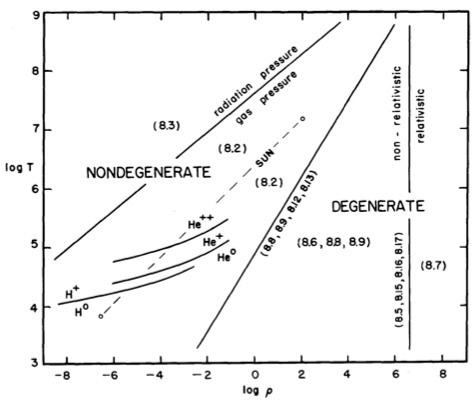
\includegraphics[width=(\textwidth),height=(\textheight-11mm),keepaspectratio]{Trho-state}
\caption{Equazione di stato nel diagramma densit\'a-Temperatura.}
\end{figure}

\subsection{Degeneracy limits}
Cerco il confine nel diagramma temperatura-densit\'a fra regione degenere e non-degenere e, nella regione degenere tra la parte relativistica e non relativistica.

Definisco il limite tra le regione degenere/non-degenere attraverso l'uguaglianza
\begin{align*}
\frac{1}{\mu_E}\frac{K}{m_P}\rho T=K_{NR}(\frac{1}{\mu_E}\rho)^{\frac{5}{3}}&\intertext{Risolvendo $\uparrow$ per la densit\'a:}\\
\frac{1}{\mu_E}\rho=(\frac{KT}{m_PK_{NR}})^{\frac{3}{2}}=2.4*10^{-8}T^{\frac{3}{2}}
\end{align*}

e il confine tra regione non-relativistica e relativiastica uguagliando la pressione data delle risp. formule
\begin{equation*}
\frac{1}{\mu_E}\rho=(\frac{K_R}{K_{NR}})^3=1.916*10^6
\end{equation*}

\subsection{Radiation/gas pressure limit}

The upper left corner represent the region where radiation pressure is dominant. The boundary line represents the equation \mblock{P_{Rad}=P_G}.

Throughout the majority of stars radiation pressure is of no importance.


\section{Electron degeneracy}

\subsection{Boltzmann statistic}

High density in volume $dV$ so that is fully pressure ionized: free electron of density $n_e$. If the velocity distro is given by Boltzmann statistic their mean kinetic energy is \mblock{\frac{3kT}{2}}: the number of electrons in spherical shell $[p,p+dp]$ is
\begin{equation*}
f(p)\,dp\,dV=n_e\frac{4\pi p^2}{(2\pi m_ekT)\expy{\frac{3}{2}}}\exp{-\frac{p^2}{2m_ekT}}\,dp\,dV
\end{equation*}

A reduction of $T$ with $n_e$ constant cause maximum of distro function $p_{max}=\sqrt{2m_ekT}$ to tends to smaller values of $p$ and the maximum of $f(p)$ becomes higher since \mblock{n_e=\intzi f(p)\,dp}

\subsection{Pauli principle}

Each quantum cell of 6D phase space can't contain more than 2 electrons with \mblock{d^3pdV=h^3}: in the shell \mblock{[p,p+dp]} of momentum space there are \mblock{4\pi p^2\,dp\,dV/h^3} quantum cells which can't contain more than \mblock{2*4\pi p^2\,dp\,dV/h^3}:
\begin{equation*}
f(p)\,dp\,dV\leq2*4\pi p^2\,dp\,dV/h^3
\end{equation*}

The Boltzmann distro for $n_e$ constant is in contraddiction with QM for low T.

\subsection{Complete degeneracy: T=0.}

The state in which all electrons have lowest energy without violating PP is that in which all phase cells are occupied up to $p_F$
\begin{align*}
&f(p)=\frac{8\pi p^2}{h^3}\ p\leq p_F\\
&f(p)=0\ p\geq p_F
\end{align*}

quindi
\begin{align*}
&n_e\,dV=dV\int_0^{p_F}\frac{8\pi p^2\,dp}{h^3}=\frac{8\pi}{3h^3}p_F^3\,dV:\\
&p_F\propto n_e\expy{\frac{1}{3}}&\intertext{non relativistic:}\\
&E_F=\frac{p_F^2}{2m_e}\propto n_e\expy{\frac{2}{3}}
\end{align*}

If density is high enough we can have velocity comparable to $c$:

\begin{align*}
&p=\frac{m_ev}{\sqrt{1-v^2/c^2}}\\
&E_{tot}=\frac{m_ec^2}{\sqrt{1-v^2/c^2}}=m_ec^2\sqrt{1+\frac{p^2}{m_e^2c^2}}
\end{align*}

Kinetic energy \mblock{E=E_{tot}-m_ec^2}

\begin{definition}{Peso molecolare medio per elettrone libero}
Mette in relazione la densit\'a col numero di elettroni liberi:
numero di \Pelectron per $cm^3$ \'e la densit\'a ($\rho$) moltiplicato moli di lettroni libero per grammo ($\frac{1}{\mu_e}$) moltiplicato $N_A\approx\frac{1}{m_p}$.
\end{definition}

\begin{usefull}{Pressure completely deg electron gas}
The pressure is the flux of momentum per unit surface per unit time: each electrons carries momentum p in direction $\hat{s}$, the component in direction $\hat{n}$ is \mblock{p\cos{\theta}}

At location of surface element there are \mblock{f(p)\,dp\,d\Omega_s/(4\pi)} electrons per unit volume with right momentum (right p and right direction): the flux of particles with \mblock{p\in[p,p+dp]} and direction within $d\Omega_s$ is  \mblock{f(p)\,dp\,d\Omega_sv(p)\cos{\theta}\,d\sigma/(4\pi)}. $\cos{\theta}$ arises since electrons moving into solid angle see only a projection of $d\sigma$.

Non relativistic pressure:
consiriomo gli \Pelectron completamente degeneri quindi lo le celle dello spazio delle fasi sono accupate con 2 elettroni fino a $p_F$ (densit\'a di stati: \mblock{\phi_e\,d^3x\,d^3p=\frac{2}{h^3}\,d^3x\,d^3p})
\mblock{P_e=\frac{8\pi}{3h^3}\int_0^{p_F}p^3v(p)\,dp}.

Relativistic:

\begin{align*}
&P_e=\frac{\pi m_e^4c^5}{3h^3}f(x)=\frac{8\pi c^5m_e^4}{3h^3}\int_0^x\frac{\xi^4\,d\xi}{\sqrt{1+\xi^2}}\\
&\xi=\frac{p}{m_ec},\ x=\frac{p_F}{m_ec}\\
&n_e=\frac{\rho}{\mu_em_u}=\frac{8\pi m_e^3c^3}{3h^3}x^3
\end{align*}


\end{usefull}

Internal energy of electron gas per unit volume:

\begin{align*}
&u_e=\int_0^{p_F}f(p)E(p)\,dp=\frac{8\pi}{h^3}\int_0^{p_F}E(p)p^2\,dp\\
&u_e=\frac{\pi m_e^4c^5}{3h^3}g(x)
\end{align*}

\subsection{Importance of relativistic effects: limiting case.}

The param \mblock{x\ (x_F=\frac{p_F}{m_ec})} is a measure of importance of relativistic effects.

\begin{usefull}{Electron degeneracy: non-relativistic limit pressure}
\begin{align*}
&x=\frac{p_F}{m_ec}=\frac{v_F/c}{\sqrt{1-v_F^2/c^2}}:\ \frac{v_F^2}{c^2}=\frac{x^2}{1+x^2}\\
&x\to0: f(x)\to\frac{8}{5}x^5,\ g(x)\to\frac{12}{5}x^5&\intertext{$x\ll1$: relativistic effects can be ignored:}\\
&P_e=\frac{1}{20}(\frac{3}{\pi})\expy{\frac{2}{3}}\frac{h^2}{m_e}n_e\expy{\frac{5}{3}}\\
&=\frac{1}{20}(\frac{3}{\pi})\expy{\frac{2}{3}}\frac{h^2}{m_em_u\expy{\frac{5}{3}}}(\frac{\rho}{\mu_e})\expy{\frac{5}{3}}\\
&=\num{1.0036e13}(\frac{\rho}{\mu_e})\expy{\frac{5}{3}}\ (cgs)\\
&P_e=\frac{2}{3}U_e
\end{align*}
\end{usefull}

\begin{usefull}{Electron degeneracy: relativistic limit pressure}
\begin{align*}
&x\to\infty: f(x)\to2x^4,\ g(x)\to6x^4&\intertext{for extreme relativistic case $x\gg1$:}\\
&P_e=(\frac{3}{\pi})\expy{\frac{1}{3}}\frac{hc}{8}n_e\expy{\frac{4}{3}}\\
&=\num{1.2435e15}(\frac{\rho}{\mu_e})\expy{\frac{4}{3}}\ (cgs)\\
&P_e=\frac{1}{3}U_e
\end{align*}
\end{usefull}

\subsection{Relazione densit\'a energia cinetica-Pressione}

Ricavo la relazione densit\'a di energia cinetica-pressione.

\begin{align*}
\epsilon=\frac{E}{V}=\frac{1}{V}\frac{3}{2}NK_BT&\intertext{Relazione tra pressione e concentrazione degli elettroni.}\\
P=\frac{2}{3}\epsilon
\end{align*}


\subsection{Degenerazione parziale}

The most probable occupation of phase cells of shell $[p,p+\,dp]$ in momentum space is determined by FD statistic
\begin{align*}
f(p)\,dp\,dV=\frac{8\pi p^2\,dp\,dV}{h^3}*\frac{1}{1+\exp{\frac{E}{KT}-\psi}}&\intertext{$\Psi$ \'e il parametro di degenerazione}
\end{align*}

\subsection{Gas di Fermi non relativistico}

\begin{itemize*}

\item Degenerazione.

\begin{equation*}
n_e\,d^3x\,d^3p\leq2\frac{d^3x\,d^3p}{h^3}
\end{equation*}

\item Densit\'a di stati.


\begin{align*}
&dN=\frac{1}{8}4\pi n^2dn&\intertext{da cui ricavo la densit\'a imponendo le condizioni periodiche al bordo del volume $V=L^3$}\\
&g(k)=\frac{dN(k)}{d^3k}=\frac{dN(k)}{4\pi k^2dk}=\frac{\nu V}{(2\pi)^3}
\end{align*}

\item Energia gas di Fermi completamente degenere: $T=0$.
\begin{align*}
&N=\int g(k)F(k)d^3k=\frac{\nu V}{(2\pi)^3}\int_0^{K_F}4\pi k^2\,dk\\
&=\frac{\nu V}{2\pi^2}\frac{k_F^3}{3}
\end{align*}
da cui ricavo la densit\'a
\begin{equation*}
n=\frac{\nu}{6\pi^2}k_F^3
\end{equation*}
e adesso introduco la densit\'a di energia e ricavo la sua dipendenza da n
\begin{align*}
&\epsilon=\frac{\hbar^2k^2}{2m_0}\quad(\epsilon_F=\frac{\hbar^2k_F^2}{2m_0})\\
&E=\int\epsilon(k)F(k)g(k)d^3k=\frac{\nu V}{2\pi^2}\frac{\hbar^2}{2m_0}\frac{k_F^5}{5}\\
&\frac{E}{N}=\frac{3}{5}\epsilon_F\\
&\epsilon=\frac{E}{V}=\frac{E}{N}\frac{N}{V}=\frac{3}{5}\epsilon_Fn\propto n^{\frac{5}{3}}
\end{align*}

\item Pressione di un gas di Fermi di elettroni completamente degenere
\begin{align*}
&P=-\frac{\partial E}{\partial V}|_{S,N}=n^2\frac{\partial(\frac{E}{N})}{\partial n}|_{S,N}\propto n^{\frac{5}{3}}\\
&P=K_{NR}\rho^{\frac{5}{3}}\\
&P=\frac{1}{20}(\frac{3}{\pi})^{\frac{2}{3}}\frac{h^2}{m_e}n_e^{\frac{5}{3}}=\frac{1}{20}(\frac{3}{\pi})^{\frac{2}{3}}\frac{h^2}{m_em_u^{\frac{5}{3}}}(\frac{\rho}{\mu_e})^{\frac{5}{3}}\\
&=1.0036*10^{13}(\frac{\rho}{\mu_e})^{\frac{5}{3}}\quad(cgs)\\
&P=\frac{2}{3}U_e
\end{align*}

\end{itemize*}

\subsection{Gas di Fermi relativistico}

\begin{itemize*}

\item Energia.

\begin{equation*}
\epsilon(k)=\sqrt{(\hbar ck)^2+(m_0c^2)^2}
\end{equation*}

\item Parametri adimensionali.

\begin{align*}
y=\frac{\hbar}{m_0c}k=\lambdabar k\\
\lambdabar k_F=x
\end{align*}

\item densit\'a di particelle.

\begin{equation*}
n=\frac{8\pi c^3m^3}{3h^3}x^3=5.87*10^{29}x^3
\end{equation*}

\item Pressione.

\begin{align*}
&P\propto n^{\frac{4}{3}}\\
&P=(\frac{3}{\pi})^{\frac{1}{3}}\frac{hc}{8}n_e^{\frac{4}{3}}=(\frac{3}{\pi})^{\frac{2}{3}}\frac{hc}{8m_u^{\frac{4}{3}}}(\frac{\rho}{\mu_e})^{\frac{4}{3}}\\
&=1.2435*10^{15}(\frac{\rho}{\mu_e})^{\frac{4}{3}}\quad(cgs)\\
&P=\frac{1}{3}U_e
\end{align*}

\end{itemize*}

\subsection{Relazione densit\'a-pressione(-impulso di Fermi) per gas degenere}

Per un gas completamente degenere di elettroni
\begin{align*}
&E_F\propto n_e^{\frac{2}{3}}&\intertext{$\uparrow$ Non-relativistico}\\
&E_F\propto n_e^{\frac{1}{3}}&\intertext{$\uparrow$ Ultra-Relativistico}
&P\propto n_e^{\frac{5}{3}}&\intertext{$\uparrow$ Non-relativistico}\\
&P\propto n_e^{\frac{4}{3}}&\intertext{$\uparrow$ Ultra-Relativistico}
\end{align*}
\index{Rivedere relazione energia fermi densita elettroni}


\subsection{Partial degeneracy}

For finite T not all electrons will be packed in momentum space in lowest possible momentum: if T is high enough we expect them to have a Boltzmann distro.

The most probable occupation of the phase cells of shell \mblock{[p,p+dp]} is determined by FD statistic
\begin{equation*}
f(p)\,dp\,dV=\frac{8\pi p^2\,dp\,dV}{h^3}=\frac{1}{1+\exp{\frac{E}{kT}-\psi}}
\end{equation*}
if $p\leq p_F$ there are fewer electrons than for $T=0$.

For non-relativistic case: $E=\frac{p^2}{2m_e}$
\begin{align*}
&n_e=\frac{8\pi}{h^3}\intzi{}\frac{p^2\,dp}{1+\exp{\frac{p^2}{2m_ekT}-\psi}}\\
&=\frac{8\pi}{h^3}(2m_ekT)\expy{\frac{3}{2}}a(\psi)\\
&a(\psi)=\intzi{}\frac{\eta^2}{1+\exp{(\eta^2-\psi)}}
\end{align*}

The degeneracy parameter is a function of \mblock{\psi(\frac{n_e}{T\expy{\frac{3}{2}}})}.

For large negative value of $\psi$, $a(\psi)$ can be made arbitrarily small: for a given electron density this is the case for high T: $f(p)$ must become Boltzmann distro and (\mblock{\frac{E}{kT}=\frac{p^2}{2m_ekT}}) \mblock{\exp{\psi}=\frac{h^3n_e}{2(2\pi m_ekT)\expy{\frac{3}{2}}}}

\section{White dwarfs}

\subsection{Grandezze caratteristiche}

\begin{itemize*}
\item $M\approx\msun$
\item $\rho_c\approx10^6gr/cm^3\approx10^4\rhosunc$.
\begin{align*}
&n_e=\exv{Z}n_I\\
&\rho=\exv{m_I}n_I+m_en_e\\
&\approx\exv{M_{atom}}n_I=\exv{A}m_Hn_I
\end{align*}

\item Raggio di Schwarzschild.

\begin{equation*}
\frac{R_G}{R}\approx100(\frac{R_G}{R})_{\odot}\approx4*10^{-6}
\end{equation*}
ho definito il raggio di Schwarzchild come $R_G=\frac{2GM}{c^2}$.
\item Velocit\'a di fuga.

\begin{equation*}
v_f=\sqrt{\frac{2GM}{R}}\approx0.02 c
\end{equation*}

\item Pressione.

\begin{equation*}
P=P_I+P_{el}\approx P_{el}
\end{equation*}
\end{itemize*}

\subsection{Application of complete degenerate statistic}

\begin{align*}
&T=0\\
&3(\gamma-1)U=-\Omega=\frac{3}{5}\frac{GM^2}{R}\\
&U=VE_e,\ E_e=12A\frac{x^5}{5}\\
&x_F=\frac{p_F}{mc},\ x(\frac{\rho}{\mu_e}),\ \rho\propto\frac{M}{R^3}\\
&n_e=\frac{8\pi}{3}(\frac{h}{m_ec})\expy{-3}x^3=\num{5.865e29}x_F^3\si{\per\cubic\cm}
\end{align*}

\begin{usefull}{WD: Non relativistic mass-radius relation}
Per densit\'a costante

\begin{align*}
&M\propto(\frac{h^2N_A}{m_eG})^3\frac{N_A^2}{\mu_e^5}\frac{1}{R^3}\\
&\frac{M}{\msun{}}\approx\num{e-6}(\frac{R}{\rsun{}})\expy{-3}(\frac{2}{\mu_e})^5
\end{align*}
Fatti:
\begin{itemize}
    \item Abbiamo assunto $P_e$, $E_e$ costanti: la maniera corretta \'e usare l'espressione generale per la pressione (\mblock{v=\PDy{p}{E_k}})
\end{itemize}
\end{usefull}



\begin{usefull}{\cha{} limiting mass}
In the limit of extreme relativistic degeneracy
\begin{equation*}
\frac{M}{\msun{}}=\frac{M_{ch}}{\msun{}}=1.456(\frac{2}{\mu_e})^2
\end{equation*}
\end{usefull}

\subsection{How far inward before degeneracy set in?}

Condizione necsuff perch\'e si abbia degenerazione \'e
\begin{align*}
\frac{4\pi^2}{(\theta mc^2)^2}\frac{x\sqrt{x^2+1}}{f(x)}\gg1&\intertext{ho definito}\\
x=\frac{h}{mc}(\frac{3n}{8\pi})^{\frac{1}{3}}\quad \theta=\frac{1}{KT}
\end{align*}
Per gli strati esterni vale $P\propto\rho T$ ($\approx0.23 \%$ della massa) 



\subsection{Equazione di stato degli Ioni}
\begin{equation*}
N_E=\frac{1}{\mu_E}\frac{\rho}{m_P}\quad\frac{1}{\mu_E}=X+\frac{1}{2}Y+\frac{1}{2}Z\approx\frac{1}{2}(1+X)
\end{equation*}

Condizioni per la degenerazione degli atomi: nuclei have on the average the same energy as electron, il momento \'e maggiore di un fattore radice quadrata del rapporto fra le masse per grado di libert\'a e quindi sono distribuiti nello spazio delle fasi su un volume $(2000)^{\frac{3}{2}}$ maggiore.
Per gli atomi possiamo usare
\begin{equation*}
P_A=\frac{1}{\mu_A}\frac{K}{m_P}\rho T\quad\frac{1}{\mu_A}=X+\frac{1}{4}Y
\end{equation*}

\subsection{Interazione Ioni-elettroni}
Il contributo Coulombiano alla pressione diminuisce la massa limite:
\begin{equation*}
P_C\propto-e^2\exv{Z}^{\frac{2}{3}}n_e^{\frac{4}{3}}<0
\end{equation*}

\subsection{Boundaries between D/ND and in latter R/NR}

Electron pressure for complete degeneracy
\begin{equation*}
P_E=\int_{|p|\leq p_0}\,d^3p\,p_xv_x\frac{2}{h^3}
\end{equation*}
e utilizzando l'opportuna relazione (R/NR) tra v e p trove la pressione nei due casi per gas di elettroni completamente degenere

\begin{itemize*}
\item Relativistico: $v=\frac{p}{m}$.
\begin{equation*}
P_E=\frac{2\pi c}{3h^3}p_0^4=K_2(\frac{\rho}{\mu_E})^{\frac{4}{3}}
\end{equation*}

\item Non relativistico $v_x=c\frac{p_x}{|p|}$.
\begin{equation*}
P_E=\frac{8\pi}{15mh^3}p_0^5=K_1(\frac{\rho}{\mu_E})^{\frac{5}{3}}
\end{equation*}

\end{itemize*}

\begin{itemize*}
\item Confine tra zona degenere e non degenere.

\begin{align*}
&\frac{1}{\mu_E}\frac{K}{m_P}\rho T=K_1(\frac{\rho}{\mu_E})^{\frac{5}{3}}\\
&\frac{1}{\mu_E}\rho=(\frac{KT}{m_PK_1})^{\frac{3}{2}}
\end{align*}

\item Confine tra zona degenere relativistica e non.

\begin{equation*}
\frac{1}{\mu_E}\rho=(\frac{K_2}{K_1})^3=1.916*10^6
\end{equation*}

\end{itemize*}

\subsection{Mass/radius relation}

L'equazioni di stato \'e indipendente da T
\begin{align*}
P=\frac{\pi m^4c^5}{3h^3}f(x)\\
\rho=\mu_E\frac{8\pi m_Pm^3c^3}{3h^3}x^3&\intertext{con}\\
x=\frac{p_0}{mc}\quad \mu_E=\frac{2}{1+X}
\end{align*}
Posso separare il problema idrostatico da quello termodinamico.

Equilibrio idrostatico:
\begin{align*}
\frac{dP}{dr}=-\rho\frac{GM_r}{r^2}\\
\frac{dM_r}{dr}=4\pi r^2\rho
\end{align*}
da integrare numericamente(Chandrasekhar).

Qualitativamente
\begin{itemize*}
\item The larger the mass of a white dwarf the smaller the radius.
\item Per nane bianche con circa massa solare il raggio \'e centinaia di volte pi\'u piccolo del sole.
\end{itemize*}

\begin{figure}[!ht]
\centering
%\includegraphics[width=(\textwidth),height=(\textheight-11mm),keepaspectratio]{MRWD}
\caption{Mass/radius relation for completely degenerate WD.}
\end{figure}

\subsection{Limite superiore per la massa di una stella completamente degenere}

Quantit\'a che influenzano l'equilibrio idrostatico:
\begin{align*}
\rho\propto\frac{M}{R^3}&\intertext{questa sopra \'e la densit\'a, questa sotto l'attrazione gravitazionale}\\
\rho\frac{GM_r}{r^2}\propto\frac{M^2}{R^5}
\end{align*}

Per la pressione:
\begin{align*}
P\propto\rho^{\frac{5}{3}}\propto\frac{M^{\frac{5}{3}}}{R^5}&\intertext{per stelle meno massive ho la pressione NR (sopra), per stelle massive uso la formula R (sotto)}\\
P\propto\rho^{\frac{4}{3}}\propto\frac{M^{\frac{4}{3}}}{R^4}
\end{align*}

il cui gradiente genera una forza di pressione
\begin{align*}
F_P&\propto\frac{M^{\frac{5}{3}}}{R^6}\quad\text{NR-D}\\
&\frac{M^{\frac{4}{3}}}{R^5}\quad\text{R-D}
\end{align*}

Osservazioni:
\begin{itemize*}
\item In the relativistic case gravitational force and pressure force depend on the same power of radius.
\item In R-D the 2 forces depend on different power of mass.
\end{itemize*}

\subsection{Massa di Chandrasekhar}

La densit\'a centrale di una nana bianca aumenta come $M^2$ fino all'istaurarsi del regime ultra-relativistico: in regime UR solo una massa \'e in equilibrio.

Usando un modello politropico ricavo
\begin{align*}
M_{Ch}=(\frac{2}{\mu_e})^2*1.459\msun&\intertext{Per nane bianche di He o C ho $\downarrow$}\\
M_{Ch}=1.4\msun
\end{align*}

Per una stella omogenea il T. del viriale ci dice
\begin{align*}
2\int\epsilon_{Cin}\,dV=\frac{3}{5}\frac{GM^2}{R}=\frac{3}{5}G(\frac{4\pi}{3})^{\frac{1}{3}}M^{\frac{5}{3}}\rho^{\frac{1}{3}}
\end{align*}

Nel caso non relativistico

\begin{align*}
&\frac{3}{5}G(3\pi^2)^{\frac{2}{3}}\frac{\hbar^2}{m_e}(\frac{1}{\mu_em_P})^{\frac{5}{3}}M\rho^{\frac{2}{3}}&\intertext{$\mu_e$ \'e il peso molecolare medio quando si considera il contributo alla pressione del gas solo degli elettroni: $\mu_e=1$ per $^1H$, $\mu_e\approx2$ per altri casi($\geq2$ adroni per elettrone). Ho usato $\downarrow$}\\
&P=\frac{1}{20}(\frac{3}{\pi})^{\frac{2}{3}}\frac{h^2}{m_e}n_e^{\frac{5}{3}}=\frac{1}{20}(\frac{3}{\pi})^{\frac{2}{3}}\frac{h^2}{m_em_u^{\frac{5}{3}}}(\frac{\rho}{\mu_e})^{\frac{5}{3}}\\
&=1.0036*10^{13}(\frac{\rho}{\mu_e})^{\frac{5}{3}}\quad(cgs)\\
&P=\frac{2}{3}U_e
\end{align*}

\begin{align*}
\rho\propto G^3(\mu_em_P)^5m_e^3M^2
\end{align*}

Nel caso relativistico

\begin{align*}
M\propto(\frac{c\hbar}{G})^{\frac{3}{2}}\frac{1}{\mu_e^2m_P^2}\to M_{Ch}
\end{align*}

\subsection{WD oscillations.}

Prendendo $\Delta R\approx1\%$:
\begin{equation*}
\Delta E_{grav}\propto \frac{GM^2}{R}\frac{\Delta R}{R}\approx\SI{e48}{\erg}
\end{equation*}

\section{Stelle di neutroni}

\subsection{Formazione}

Nascono dal collasso di una stella ed hanno $T\geq10^{10}\,K$: rapidamente la temperatura della stella diminuisce a causa del flusso di neutrini. In 100 yr $T\approx10^8$, che pu\'o essere considerata bassa vista l'energia massima dei neutroni altamente degeneri:
\begin{align*}
KT\approx10\,KeV\\
E_F\approx1000\,MeV
\end{align*}
L'equazione di stato \'e essenzialmente la stessa che per $T\approx0$.

\subsection{Neutronizzazione}

L'aumento della densit\'a aumenta l'energia degli elettroni che danno luogo con i protoni a electron capture. I nuclei arricchiti di neutroni ($^{118}Kr$) cominciano ad emetterli a una densit\'a $\rho_{dr}\approx4*10^{11}g/cm^3$.\index{Neutron drip}

In questo stadio la materia \'e composta da nuclei (di solito organizzati in reticolo), elettroni e neutroni liberi: il numero di elettroni aumenta con la densit\'a e cos\'i $P_n$.

\begin{align*}
P\approx P_e\gg P_n&\intertext{$\uparrow$ per $\rho\approx\rho_{dr}$}\\
p_n\approx\frac{P}{2}&\intertext{$\uparrow$ per $\rho\approx10^{12}gr/cm^3$}
\end{align*}

\subsection{Fasi successive: Hyperionizzation.}

A partire dall densit\'a per cui i nuclei sono in contatto $\rho_{Nuc}\approx2.4*10^{14}gr/cm^3$ ho un gas/liquido di neutroni degeneri in equilibrio con piccola frazione di \Pproton, \Pelectron: $\Pneutron\leftrightarrow\Pproton+\Pelectron$. 

Successivamente ho iperionizzazione e quark liberi.

\subsection{Massa limite per stelle di neutroni}

Uso i conti fatti per le nane bianche con opportuno scaling

\begin{align*}
m_e\to m_n\\
\underbrace{\mu_{WD}}_2\to\underbrace{\mu_{NS}}_1\\
\end{align*}

ottengo

\begin{align*}
&\rho^{NS}(M)=\rho^{WD}(M)(\frac{m_n}{m_e})^3(\frac{\mu_{NS}}{\mu_{WD}})^5\\
&\approx2.5*10^8\rho^{WD}(M)\\
&\rho^{NS}(M)\approx2.5*10^{14}(\frac{M}{\msun})^2g/cm^3
\end{align*}

e per la massa limite di una stella di neutroni ottengo
\begin{equation*}
M_{Cha}^{NS}=M_{Cha}(\frac{\mu_{WD}}{\mu_{NS}})^2\approx5.7\msun
\end{equation*}
Calcoli pi\'u precisi abbassano il limite?

\section{Buchi neri}

\subsection{Raggio di Schwarzschild}

Alla superficie di una configurazione di massa M e raggio R la curvatura gaussiana dello spazio \'e 
\begin{align*}
&K_G=\frac{GM}{c^2R^3}=-\frac{1}{2}\frac{r_s}{R}\frac{1}{R^2}&\intertext{\'e solitamente piccolo rispetto alla curvatura $R^{-2}$ della superficie sferica:}\\
&-K\approx2*10^{-6}\frac{1}{R^2}&\intertext{$\uparrow$ at surface of the sun}\\
&-K\approx0.15\frac{1}{R^2}&\intertext{$\uparrow$ for neutron star}\\
&-K\approx\frac{1}{R^2}&\intertext{$\uparrow$ for black hole with $R=r_s$}
\end{align*}

Il parametro critico \'e il raggio di Schwarzschild
\begin{equation*}
r_s=\frac{2MG}{c^2}
\end{equation*}
cio\'e la distanza dal centro di attrazione di una massa per cui $v_f=c$.

\subsection{Densit\'a critica}

In termini di densit\'a ho
\begin{align*}
\rho_{Crit}\approx2*10^{16}(\frac{\msun}{M})^2g/cm^3
\end{align*}

\part{Modello ed evoluzione stellare.}
\chapter{Formation of a star from interstellar medium}
\PartialToc

\section{Broader problem of formation of a star}
(Burbidge (1960), Kahn (1960), Ebert-von Hoerner-Temesvary (1960))

Change in density from \SIrange{e-24}{1}{\gram\per\cubic\cm}

\section{Final stage of formation}
A star without neclear reactions:
\begin{itemize}
\item Optically thick system: radiation escapes only from thin surface layer
\item Hydrodynamic time-scale must be much shorter than thermal time-scale: we can calculate heat flow assuming HE.
\end{itemize}
 
\subsection{Conditions for homologous contraction}

$\TDly{\rho}{T}$: in a log-plot of temperature vs density profile during contraction every point evolve parallel to the $p_g=P_r$ line.

\chapter{Fonti energia: energia gravitazionale ed energia interna.}

A star derives its energy to shine from internal energy, thermonuclear fuel, and gravitational contraction.
\PartialToc


\section{Equilibrio meccanico locale vs constrain on star's structure}

\subsection{G-nal potential energy}
(vedi ~\ref{chap:gravity}) L'energia potentziale gravitazionale di un corpo autogravitante \'e l'opposto dell'energia necessaria per portare le masse infinitesime arbitrariamente lontane:
\begin{align*}
&d\Omega=-\int_r^{\infty}\frac{Gm(r)}{r'^2}\,dm(r)\,dr'\\
&=-\frac{Gm(r)}{r}\,dm(r)\\
&\Omega=-\int_0^M\frac{Gm(r)}{r}\,dm(r)\\
&\Omega=-q\frac{GM^2}{R}&\intertext{per densit\'a uniforme}\\
&\Omega=-\frac{3}{5}\frac{GM^2}{R}
\end{align*}

\subsection{\kh{} time-scale (sole)}
Nel caso del sole: divido l'energia potentziale G-nal per la luminosit\'a attuale
\begin{equation*}
\frac{G\msun}{\rsun}\approx\num{3.8e48}\si{\erg}/\lsun\approx\num{3e7}\,yr
\end{equation*}

\subsection{Mechanical and internal energy}

Trascuro i moti macroscopici o fenomeni turbolenti: l'energia totale di una stella

\begin{align*}
&W=\int_ME\,dm(r)+\Omega=U+\Omega\\
&U=\int_ME\,dm(r)
\end{align*}

\subsection{Equilibrium state. Adiabatic perturbation.}

Equilibrium state of the star corrisponds to extrema of $W$: hydrostatic equilibrium is an extremum relative to other configurations.

For adiabatic perturbation (abbastanza rapide da pater trascurare gli scambi di calore e abbastanza lente da poterne trascurare l'energia cinetica, adiabatic sound waves) 

\begin{align*}
&\varad{W}=0&\intertext{$\uparrow$ hydrostatic stellar equilibrium}\\
&\varad{W}=\varad{U}+\varad{\Omega}\\
&U\to U+\varad{U}=U+\delta\int_ME\,dm(r)\\
&=U+\int\delta E\,dm(r)&\intu{changes in specific internal energy of a particular mass element $dm(r)$ (Lagrangian description of the perturbation).}
\end{align*}

We label each mass element of $dm(r)$ worth of matterand see what happens to $E$ when $r$, $T$ and $\rho$ change.

\begin{align*}
&dQ=dE+P\,d\vrho{}=T\,dS&\intu{1 e 2 leggi termodinamica}\\
&\vrho=\frac{1}{\rho}
\end{align*}
Qui scrivo $\vrho{}$ per indicare il volume specifico con dimensioni \si{\cubic\cm\per\gram} cio\'e il volume associato ad 1 grammo di materia:
\begin{align*}
&\vrho{}=\frac{1}{\rho}=\frac{4\pi r^2\,dr}{dm(r)}=\frac{d(\frac{4\pi r^3}{3})}{dm(r)}\\
&\vrho{}\to\vrho{}+\var{\vrho{}}=\frac{d[4\pi\frac{(r+\var{r})^3}{3}]}{dm(r)}\vrho{}\\
&+\frac{d(4\pi r^2\var{r})}{dm(r)}&\intu{al primo ordine in $\var{r}$: $\frac{\var{r}}{r}\ll1$ and ''spherically symmetric'' perturbation.}
\end{align*}

\begin{align*}
&\varad{U}=-\int_MP\var{\vrho{}}\,dm(r)\\
&=-\int_MP\TDof{m_r}(4\pi r^2)\,dm_r\\
&\varad{U}=\int_M\TDy{m_r}{P}4\pi r^2\var{r}\,dm_r&\intu{Boundary conditions:}\\
&\var{r}(m_r=0)=0,\quad P_S=P(m_r=M)=0\\
\end{align*}

Per l'energia potenziale gravitazionale
\begin{align*}
&\Omega\to\Omega+\var{\Omega}=-\int_M\frac{Gm_r}{r+\var{r}}\,dm_r=\\
&\approx\Omega+\int_M\frac{Gm_r}{r^2}\var{r}\,dm_r
\end{align*}

\begin{align*}
&\varad{W}=\int_M[\TDy{m_r}{P}4\pi r^2+\frac{Gm_r}{r^2}]\,\var{r}\,dm_r&\intertext{condizione necessaria per l'equilibrio idrostatico:}\\
&\varad{W}=0\Leftrightarrow\TDy{m_r}{P}=-\frac{Gm_r}{4\pi r^4}&\intu{condizione di equilibrio idrostatico}
\end{align*}

\subsection{Significance of second variation of $W$}
(Cole Miller Maryland)
\begin{itemize*}
\item EOS: $P=c_1\rho\expy{\Gamma_1}$
\item write $\svarad{W}$
\item Change variable: $m_r\to V$ (terms like $\var{r}^2$ in term of $V$ and $\var{V}$)
\item if $\gamma_1$ constant throughout the star $\var{V}=kV$
\item Simplify $\svarad{W}>0$
\end{itemize*}

\section{Virial theorem}

\subsection{Virial theorem}

\begin{align*}
&\frac{1}{2}\TtwoDy{t}{I}=2K+\Omega\\
&I=\sum m_ir_i^2,\quad 2K=\sum m_iv_i^2=\sum\scap{p_i}{v_i}&\intertext{Derived for sum or integral over the whole star: if we had chosen a sphere of radius $R'<R$ the material contained within the shell $R'<r<R$ would contribute with additional term on the rhs $-3P_SV_S$ where are defined pressure at radius $R'$ and volume in same radius.}
\end{align*}


\subsection{Energia totale}

\begin{align*}
&2K=\sum m_iv_i^2=\sum\scap{p_i}{v_i}&\intu{Is it U or differs? The scala product $\scap{p_i}{v_i}$ measures the momentum transfer hence must be related to Pressure.}\\
&P=\frac{1}{3}\int n(\vec{p})\scap{v}{p}\,d^3p&\intu{$n(\vec{p})$ (dimension \si{\per\cubic\cm\per\cubic\momentum}) is the number density of particles with momentum $\vec{p}$, in the continuum limit for isotropic gas.}\\
&2K=3\int_VP\,dV\quad\Rightarrow\quad 2K=3\int_M\frac{P}{\rho}\,dm_r&\intu{ho usato che}\\
&dm_r=\rho d(\frac{4}{3}\pi r^3)\rho\,dV\\
&\frac{1}{2}\TtwoDy{t}{I}=\int_M\frac{3P}{\rho}+\Omega
\end{align*}

\subsection{$\gamma$-law equation of state}

\begin{align*}
&P=(\gamma-1)\rho E&\intertext{E is energy per uni mass (\si{\erg\per\gram}), for a monoatomic ideal gas:}\\
&\gamma=\frac{c_P}{c_V}=\frac{5}{3},\quad P=\frac{2}{3}\rho E&\intertext{for radiation or completely relativistic Fermi gas:}\\
&\gamma=\frac{4}{3},\quad K=\frac{3}{2}(\gamma-1)U&\intertext{$K=U$ only for $\gamma=\frac{5}{3}$: total kinetic energy is the same as the total internal energy only under certain circumstances ($\gamma=\frac{5}{3}$ doesn't mean necc the gas is ideal and monotonic).}
\end{align*}

Relation between W and $\Omega$ for hydrostatic stars
\begin{align*}
&\frac{1}{2}\TtwoDy{t}{I}=3(\gamma-1)U+\Omega\\
&\frac{1}{2}\TtwoDy{t}{I}=3(\gamma-1)W-(3\gamma-4)\Omega&\intertext{for hydrostatic equilibrium:}\\
&W=\frac{3\gamma-4}{3(\gamma-1)}\Omega&\intertext{hydrostatic equilibrium and dynamically stable: $W<0$ and so $\gamma>\frac{4}{3}$.}
\end{align*}

\subsection{Contracting star}

Very gradually mantaining sphericity and hydrostatic eq all time (almost)
\begin{align*}
&\Delta W=\frac{3\gamma-4}{3(\gamma-1)}\Delta\Omega&\intertext{$\gamma>\frac{4}{3}$ costante.}\\
&\Omega\propto-\frac{GM^2}{R}\Rightarrow\mvar{\Omega}\propto\frac{GM^2}{R^2}\mvar{R}&\intertext{$\mvar{\Omega}<0$ e dal viriale risulta $\mvar{W}<0$ cio\'e il sistem ha perso energia:}\\
&\mvar{U}=-\frac{1}{3(\gamma-1)}\mvar{\Omega}&\intertext{$\mvar{U}>0$ for contraction: the star heat up, the rest of energy made available by contraction $|\mvar{W}|$ is lost from the system.}
\end{align*}

For ideal gas with $\gamma=\frac{5}{3}$
\begin{equation*}
\mvar{W}=\frac{1}{2}\mvar{\Omega}=\frac{q}{2}\frac{GM^2}{R^2}\mvar{R}
\end{equation*}

Ipotiziamo che la variazione di energia totale per unit\'a di tempo sia uguale in valore assoluto uguale alla luminosit\'a della stella
\begin{align*}
&L=-\TDy{t}{W}=-\frac{q}{2}\frac{GM^2}{R}(\frac{1}{R}\TDy{t}{R})&\intertext{If L is constant we have an e-folding time:}\\
&\tkh{}\approx\frac{q}{2}\frac{GM^2}{LR}\\
&\tkh{}(q\approx\frac{3}{2})\\
&\approx\num{2e7}(\frac{M}{\msun{}})^2(\frac{L}{\lsun{}})\expy{-1}(\frac{R}{\rsun{}})\expy{-1}\,yr&\intertext{this q value is representative for the sun}
\end{align*}

\section{Gravitational energy generation rate}

\subsection{Thermal balance}

For a given \si{\gram} of material the local rate of thermonuclear energy generation is balanced by mass divergenge of luminosity
\begin{equation*}
\PDy{m_r}{l_r}=\epsilon,\quad [\epsilon]=\si{\erg\per\gram\per\second}
\end{equation*}

If the equality doesn't hold the energy content varies
\begin{align*}
&\TDy{t}{Q}=\PDy{t}{E}+P\PDof{t}(\frac{1}{\rho})=\epsilon-\PDy{m_r}{l_r}&\intertext{$Q$ is the heat content in \si{\erg\per\gram} (Lagrangian mode: a particular gram of matter is followed in time).}\\
&\PDy{m_r}{l_r}=\epsilon+\epsilon_g\\
&\epsilon_{g}=-[\PDy{t}{E}+P\PDof{t}(\frac{1}{\rho})]\\
&\epsilon_g=-\frac{P}{\rho(\Gamma_3-1)[\PDy{t}{\ln{P}}-\Gamma_1\PDy{t}{\ln{\rho}}]}&\intu{for $\Gamma_1$ constant in time: vedi \cite{cox68stellar} $\S 17.6$.}\\
&\epsilon_g=-\frac{P}{\rho(\Gamma_3-1)}\PDof{t}[\ln{\frac{P}{\rho\expy{\Gamma_1}}}]
\end{align*}

\subsection{Departures from adiabaticity}

$\epsilon_g=0$ for adiabatic process where $P\propto\rho\expy{\Gamma_1}$: energy release in gravitational sources arises from departures from adiabaticity during contraction or expansion. If the pressure rises less than adiabatic upon compression $P\propto\rho\expy{\Gamma_1-\delta}$ then $\epsilon_g=\delta\frac{P}{\rho(\Gamma_3-1)}\PDy{t}{\ln{\rho}}>0$: a less than adiabatic rise of pressure upon compression implies that energy is being released by $P\,dV$ work ($dq=du+P\,dV$).


\chapter{Modelli Stellari.}
\PartialToc

\section{Teorema Vogt-Russel}

In those cases where VR theorem is not valid (where specification of M and chemical composition fails to determine a model uniquely) some information about star's evolution history are needed.

\subsection{Usefull rule of thumb}

Complete structure of a star in hydrostatic and thermal equilibrium is uniquely determined by total mass and run of chemical composition throughout the star: provided pressure, internal energy per unit mass, opacity, and energy generation rate are functions only of density, temperature and chemical composition.

\subsection{Order of magnitude estimates: theoretical relation between fundamental parameter.}

Let us consider a star of mass M and radius R in HE:
\begin{align*}
&\rho=\frac{M}{R^3}\\
&P\approx G\frac{M^2}{R^4}&\intertext{internal pressure must be great enough to support weight of overlying layers,}\\
&T=\frac{\mu}{\gasconstant{}}\frac{P}{\rho}\approx\frac{G}{\gasconstant{}}\frac{\mu M}{R}&\intertext{specification of equation of state further determine T. There is an energy outflow: for a given temperature gradient the luminosity is determined by opacity (assuming radiative transport), in diffusion approximation:}\\
&\TDof{r}(\frac{1}{3}aT^4)=-\frac{\kappa\rho}{c}\frac{l}{4\pi r^2}\\
&L_{rad}\approx\frac{4\pi ac}{3}R^2\frac{T^4}{R}\frac{1}{\kappa\rho}=\frac{4\pi ac}{3}R\frac{T^4}{\kappa\rho}\\
&=\frac{4\pi ac}{3}(\frac{G}{\gasconstant{}})^4\frac{\mu^4M^3}{\kappa}&\intertext{Per l'opacit\'a introduco la legge di Kramer:}\\
&\kappa=\kappa_0\rho T\expy{-3.5}\\
&=\kappa_0(\frac{\gasconstant{}}{G})\expy{3.5}\frac{R\expy{0.5}}{\mu\expy{3.5}M\expy{2.5}}
\end{align*}

\begin{usefull}{Mass-Luminosity law (theoretical)}
\begin{align*}
&L_{rad}=\frac{4\pi ac}{3}(\frac{G}{\gasconstant{}})^4\frac{\mu^4M^3}{\kappa}&\intu{appropriate for constant opacity (Thomson scattering by free electron)}\\
&L_{rad}=\frac{4\pi ac}{3\kappa_0}(\frac{G}{\gasconstant{}})\expy{7.5}\frac{\mu\expy{7.5}M\expy{5.5}}{R\expy{0.5}}&\intertext{appropriate for Kramer's opacity law}
\end{align*}

\end{usefull}


L is determined only by M and chemical composition ($\mu$, $\kappa_0$) and weakly by R. Nuclear energy sources influence mass distribution but usually is a small effect.

\begin{usefull}{Radius-$L_{nucl}$ relation}
Now we use the condititon of thermal equilibrium
\begin{align*}
&L_{gen}=\int_0^M\epsilon\,dm\approx\epsilon M&\intertext{for a star burning hydrog via carbon cycle}\\
&\epsilon=\epsilon\rho T\expy{17}\\
&L_{gen}\approx\epsilon_0(\frac{G}{\gasconstant{}})\expy{17}\frac{\mu\expy{17}M\expy{19}}{R\expy{20}}
\end{align*}
\end{usefull}

The condition of thermal equilibrium $L_{gen}=L_{rad}$ uniquely determines R for given chemical composition and mass.


\section{Modello omogeneo in equilibrio}

Treatment of homologous stars using dimensional analysis.

\subsection{Homologous stars}

Sequences of stellar models in complete equilibrium where one is related to the other by a simple change in scale: all have the same constituent physics, the same uniform composition and that, chosen a reference in the sequences indicated with $0$ subscript
\begin{align*}
&r=\frac{R}{R_0}r_0\\
&m_r=\frac{M}{M_0}m_{r0}
\end{align*}

\subsection{Energy generation/transport: power law constitutive equations.}

Indico la produzione di energia per grammo in un guscio sferico $dm_r$ e spessore $dr$ con $\epsilon$ (\si{\erg\per\second\per\gram}).
\begin{align*}
&l(r+\,dr)-l(r)=dl(r)=4\pi r^2\rho\epsilon\,dr=\epsilon\,dm(r)\\
&\PDy{r}{l(r)}=4\pi\rho r^2\epsilon,\quad\TDy{l_r}{m_r}=\epsilon&\intertext{Thermal balance, energy equation}
\end{align*}

Power law for $\epsilon$
\begin{align*}
&\epsilon=\epsilon_0\rho\expy{\lambda}T\expy{\nu}\\
&\lambda=1,\quad \nu\approx4&\intertext{pp-chains}\\
&\lambda=1,\quad \nu\approx15&\intertext{CNO cycles}\\
&\lambda=2,\quad \nu\approx40&\intertext{Triple-$\alpha$}
\end{align*}

In the interior of the stars the energy flux obey to Fick's law of diffusion $F(r)=-D\TDy{r}{(aT)^4}$
\begin{align*}
&l(r)=-\frac{4\pi r^2c}{3\kappa\rho}\TDy{r}{aT^4}\\
&l_r=-\frac{(4\pi r^2)^2c}{3\kappa}\TDy{m_r}{aT^4}\\
&\kappa=\kappa_0\rho^nT\expy{-s}\si{\square\cm\per\gram}
\end{align*}

\subsection{Stellar dimensional analysis}
Simple treatment  of homologous stars using dimensional analysis 

\begin{align*}
&P\propto\frac{M^2}{R^4}&\intertext{Lagrangian form hydrostatic equilibrium}\\
&P_0=\rho\expy{\chi_{\rho}}T\expy{\chi_T}\\
&d\ln{P}=\chi_{\rho}\,d\ln{\rho}+\chi_T\,d\ln{T}&\intertext{$\chi_{\rho}$ and $\chi_T$ are assumed to be the same for all the stars in the collection.}
\end{align*}

\subsection{Energy, hydrostatic, diffusive radiative, constitutive equations: power law.}

\begin{align*}
&R\propto M^{\alpha_R}\\
&\rho\propto M^{\alpha_{\rho}}\\
&T\propto M^{\alpha_T}\\
&L\propto M^{\alpha_L}
\end{align*}

We insert the above relations in the equilibrium equation in differential form

\subsubsection{Radiative energy transfer}
\begin{align*}
&
\begin{pmatrix}
3&1&0&0\\
4&\chi_{\rho}&0&\chi_T\\
0&\lambda&-1&\nu\\
4&-n&-1&4+s\\
\end{pmatrix}
\begin{pmatrix}
\alpha_R\\
\alpha_{\rho}\\
\alpha_L\\
\alpha_T\\
\end{pmatrix}
=\begin{pmatrix}
1\\2\\-1\\1\\
\end{pmatrix}
\end{align*}

The solutions are
\begin{align*}
&\alpha_R=\frac{1}{3}[1-2\frac{\chi_T+\nu-s-4}{D_{rad}}]\\
&\alpha_{\rho}=2\frac{\chi_T+\nu-s-4}{D_{rad}}\\
&\alpha_L=1+2\frac{2\lambda(\chi_T+\nu-s-4)-2\nu(\chi_{\rho}+\lambda+n)}{D_{rad}}\\
&\alpha_T=-2\frac{\chi_{\rho}+\lambda+n}{D_{rad}}
\end{align*}

\subsubsection{Convective energy transfer}

If energy transport is convective we can use (altough the result are of limited use)
\begin{align*}
&T(r)\propto\rho(r)\expy{\Gamma_3-1}\\
&\Gamma_3-1=\Dcad{\TDly{\rho}{T}}
\end{align*}

quindi
\begin{align*}
&
\begin{pmatrix}
3&1&0&0\\
4&\chi_{\rho}&0&\chi_T\\
0&\lambda&-1&\nu\\
0&\Gamma_3-1&0&-1\\
\end{pmatrix}
\begin{pmatrix}
\alpha_R\\
\alpha_{\rho}\\
\alpha_L\\
\alpha_T\\
\end{pmatrix}
=\begin{pmatrix}
1\\2\\-1\\1\\
\end{pmatrix}
\end{align*}


\subsection{Sequenza principale. Relazioni semi-empiriche.}
The stars we think we know the most about are located on the hydrogen main sequence.

\subsubsection{Massive stars}
The stars on the upper massive luminous part of main sequence have higher central temperature

The opacity is determined by electron scattering so $n=s=0$. The energy is generated by CNO cycle so $\lambda=1$, $\nu\approx15$.
Radiative transport of energy dominates the outer part and pressure is largely determined by ideal gas law for which $\chi_{\rho}=\chi_T=1$. Confronto fit dati osservativi/equazioni stelle omologhe (the Sun appears as reference in the homologous set of stars.)
\begin{align*}
&\alpha_R=0.78,\quad\alpha_L=3.0&\intu{exponent calculated using  homologous relations,}\\
&\frac{R}{\rsun{}}\approx(\frac{M}{\msun})\expy{0.75},\quad\frac{L}{\lsun{}}\approx(\frac{M}{\msun{}})\expy{3.5}&\intu{data fit for stellar mass greater than few solar masses;}\\
&\alpha_T=0.22,\quad\alpha_{\rho}=-1.33&\intu{in upper main sequence T should increses with mass whereas density should decrese.}
\end{align*}

\subsubsection{Lower MS (Less Massive stars)}
Is more difficult to treat. The pp-chain dominate energy generation and Kramer's opacity operates for much of the star, convection is important especially for low mass stars. Structure of these stars is determined by what happens at very outermost radiative surface.

Empirically result $\alpha_L\approx3.9$ where the homologous equations predict 5.5.


\section{Modello standard del sole}

\subsection{Il sole.}

\begin{align*}
&\msun=2*10^{33}gr\\
&\text{Age}=4.55*10^9\,yr\\
&\rsun=7*10^5 Km\\
&\tsunc=1.57*10^7 K\\
&\tsuns=6*10^3 K\\
&\rhosunc=130gr/cm^3\\
&\lsun=3.8*10^{26}W=3.8*10^{33}erg/s\\
&\Phi_{\nu}(\Pproton\Pproton)=6.0*10^{10}cm^{-2}s^{-1}\\
&\Phi_{\nu}(^8B\to^8Be^*+\APelectron+\Pnue)=6.0*10^6cm^{-2}s^{-1}\\
&X=74\%,\,Y=23,\,Z=3&\intertext{$\uparrow$ Attuale}\\
&X=75\%,\,Y=22,\,Z=3&\intertext{$\uparrow$ Composizione iniziale}\\
\end{align*}

\subsection{Equilibrio idrostatico.}
\begin{align*}
&dS\,(P(r)-P(r+\,dr)-F_g(r))=0\\
&F_g(r)=G\frac{m(r)\rho(r)\,dV}{r^2}&\intertext{se ho simmetria sferica}\\
&\frac{dm}{dr}=4\pi\rho(r)r^2
\end{align*}

Posso trascurare la BE gravitazionale?
\begin{align*}
&B_{\odot}=N_Pm_p-\msun=-E_G=\frac{3}{5G\frac{\msun^2}{\rsun}}\\
&\approx10^{-6}\msun c^2
\end{align*}

\subsection{Equazione di stato.}

\begin{align*}
&P=P(\rho,T,X,Y,Z)=P_{Gas}+P_{Rad}&\intertext{Gas ideale}\\
&P_{Gas}=K\rho T\\
&P_{Rad}=\frac{1}{3}aT^4
\end{align*}

\subsection{Produzione di energia}
\begin{align*}
\epsilon=\frac{\text{Energia prodotta}}{\text{Massa}*\text{Tempo}}&\intertext{L'energia prodotta per fusione}\\
\epsilon=\epsilon_F(\exv{\sigma v},\rho,T,X,Y,Z)&\intertext{\'e legata alla luminosita tramite}\\
\frac{d\lu}{dr}=\epsilon_F(r)4\pi r^2
\end{align*}

\subsection{Reaction Rate}
La radiazione che raggiunge la terra ha un flusso di $1.4*10^3 W/m^2$ quindi la potenza irraggiata \'e $4*10^{26} W$: dato che ogni reazione di fusione libera 25 MeV sono necessarie $10^{38} \text{Fusioni}/sec$ (4 $^1H$ per fusione).

\begin{equation*}
N_{Reaz}=\frac{\exv{R_{PP}}}{n_P}N_p(core)
\end{equation*}

\subsection{Flusso neutrini}
\begin{equation*}
\Phi_{\nu}=\frac{\dot{N_{\nu}}}{4\pi d^2}=7*10^{10}\frac{\Pnu}{s*cm^2}
\end{equation*}



\chapter{Modello stellare. Fasi evoluzione stellare.}
\PartialToc

\section{Modellizzazione stellare rappresentata nel diagramma di \hr{}.}


\subsection{Subdwarf}

\begin{figure}[!ht]
\centering
%\includegraphics[width=(0.99\textwidth),height=(\textheight),keepaspectratio]{subdwarfHR}
\caption{\hr{} diagram of sub dwarf model.}
\end{figure}

\begin{figure}[!ht]
\centering
%\includegraphics[width=(0.99\textwidth),height=(\textheight),keepaspectratio]{subdwarftable}
\caption{Characteristic of $0.6\msun{}$ and $1\msun{}$ sub dwarf model.}
\end{figure}

\clearpage

\subsection{Main sequence}

\begin{figure}[!ht]
\centering
%\includegraphics[width=(0.99\textwidth),height=(0.9\textheight),keepaspectratio]{MSband}
\caption{Position in M-L diagram during MS for metal rich stars. L and M are in solar units. Lower curve defines locus of homogeneous initial MS model. Number in parenthesys are \mblock{(\rho,T_6,R,\frac{M_{conv-core}^{Max}}{M},\tau_{MS})}}
\end{figure}


\clearpage

\subsection{Stellar evolution}

\begin{figure}[!ht]
\centering
%\includegraphics[width=(0.99\textwidth),height=(\textheight),keepaspectratio]{PMSevotrack}
\caption{Post MS track for population I stellar models.}
\end{figure}


\begin{figure}[!ht]
\centering
%\includegraphics[width=(0.99\textwidth),height=(\textheight),keepaspectratio]{PMSevotrack}
\caption{Post MS track for population I stellar models.}
\end{figure}
ETlowmass
fiveMsunevo
evolutionMvar
timeMvar
PMSevotrack
\clearpage

\section{Composizione chimica.}

\subsection{Metallicit\'a.}
L'assenza di fusione negli strati superficiali delle stelle da dove si originano le righe fa supporre  che la loro composizione sia quella iniziale, a parte fenomeni di dredge up e sedimentazione.

La somma degli elementi pi\'u pesanti di He cresce passando da Pop. II a Pop. I.

\subsection{Formazione iniziale di metalli.}

Modelli cosmologici prevedono $Z_{in}<\num{e-6}$ mentre le stelle pi\'u vecchie osservate mostrano Z maggiore di circa 3 ordini di grandezza.

\subsection{Nucleosintesi.}
Primordial elements: they carry cosmological informations.

Prima ipotesi: decadimento di $\Pneutron\to\Pproton$ would initiates chain of neutron captures.

Von Weizsacker: nucleosynthesis in the context of stars evolutions.

Primordial fire-ball may have produced many of lightest elements but most of those with nuclear charge $Z\geq6$ are ashes of nuclear burning during stellar evolution.

Heavy elements in extreme pop II object are less abundant compared to H than they are in pop I by a factor $>100$.

He is absent in extreme popII stars.

\subsection{Galaxy chemical composition.}

If no concentration mechanism exists than the galaxy has synthetized $99\%$ of its own heavy elements.

If galaxy formed with significant abundance of He and rare elements ($D\indices{^2},He\indices{^3},Be\indices{},B\indices{}$) it must be interpreted as residual of earlier history.

\subsection{Synthesis at stellar surface.}

Non-thermal events: spallation of heavier nuclei by energetic flare particles or shock phenomena in supernovae envelopes.

\subsection{Produced in early phase of stars formations.}


\section{Fasi finali dell'evoluzione stellare.}

\subsection{Teorema del viriale}
Relazione tra l'energia cinetica media e l'energia potenziale di un sistema in equlibrio stabile o quasi-stabile.

\begin{align*}
&G=\sum_i\scap{p_i}{r_i}=\frac{1}{2}(\sum_im_ir_i^2)^2=\frac{1}{2}\frac{dI}{dt}&\intertext{I momento d'inerzia}\\
&\frac{dG}{dt}=\sum_i\scap{\dot{r_i}}{p_i}+\sum_i\scap{r_i}{\dot{p_i}}=2T\\
&+\sum_i\scap{r_i}{f_i}&\intertext{l'ultimo termi del membro di destra \'e il  viriale di Clausius}\\
&\intertext{Assumendo che la forza tra le particelle segua una legge di potenza della distanza con esponente n(del potenziale) e sia derivabile da un potenziale}\\
&\frac{dG}{dt}=2T-n\mathcal{U}&\intertext{dove U \'e l'energia potenziale totale del sistema}\\
&\frac{dG}{dt}=\frac{1}{2}\frac{d^2I}{dt^2}=2T+\Omega&\intertext{per il potenziale gravitazionale n=-1}\\
&2\overline{T}+\overline{\Omega}=0&\intertext{se il sistema \'e periodico la media del lato sinistro su un periodo dell'equazione sopra \'e nullo}
\end{align*}

\subsection{Fasi di contrazioni ed espansioni successive.}

Terminato l'idrogeno il core di elio si contrae non essendoci pi\'u fonti di energia fino a che si raggiungono T sufficienti per la fusione di dell'elio.

Detti m massa del core e r suo raggio
\begin{align*}
&E_G=-G\frac{m^2}{r}&\intertext{quindi in fase di contrazione}\\
&\Delta E_G=\frac{Gm}{r^2}\Delta r<0&\intertext{da cui risulta aumento di energia cinetica}\\
&\Delta E=-\frac{1}{2}\Delta U_G>0
\end{align*}

\subsection{fase di fusione dell'elio ($T\approx10^8K$).}

Fusione di elio-4 in carbonio-12
\begin{align*}
&^4He+^4He\to ^8_4Be\quad(\tau\approx10^{-16}s)\\
&^8Be+^4He\to^{12}C+\gamma&\intertext{al crescere di T}\\
&^{12}C+^4He\to ^{16}O+\gamma\\
&^{16}O+^4He\to^{20}Ne+\gamma
\end{align*}

\subsection{Fase di fusione del carbonio-12.}

\begin{align*}
^{12}C+^{12}C&\to ^{16}O+2^4He\\
&\to ^{20}Ne+^4He\\
&\to ^{23}Na+\Pproton\\
&\to^{24}Mg+\gamma
\end{align*}

\subsection{Fase fusione Ossigeno.}
\begin{align*}
^{16}O+^{16}O&\to ^{28}_{14}Si+^4He\\
&\to^{31}_{15}P+\Pproton\\
&\to ^{32}S+\gamma
\end{align*}

e cos\'i via fino al $^{56}Fe$ per le stelle pi\'u massicce.

\subsection{Destino finale della stella}

\begin{itemize*}
\item $M<8\msun$: Nane bianche ($R\approx R_T$).
La pressione di degenerazione degli elettroni blocca il collasso.

\item $8\msun<M<25\msun$: stella di neutroni.
La nucleosintesi raggiunge il $^{56}Fe$  poi hanno luogo fenomeni di cattura elettronica (neutronizzazione della materia): sintesi elementi pi\'u pesanti.

\item $M>25\msun$: buco nero.

\end{itemize*}


\chapter{Modelli di Stelle politropi}
\PartialToc.


\section{Polytropic gaseous spheres}

\subsection{Polytropic changes.}

\begin{definition}{Polytropic changes.}
Un elemento di materia subisce una trasformazione politropica se $dQ=cdT$ con c costante o pi\'u in generale se durante il processo di stirring la quantit\'a di calore $dQ$ fornita \'e proporzionale alla variazione istantanea di temperatura.

\begin{align*}
&(c_v-c)\,dT+P\,dV=0\\
&(c_V-c)\frac{dT}{T}+(c_p-c_V)\frac{dV}{V}=0\\
&P=K\rho\expy{\gamma'}\\
&\gamma'=\frac{c_P-c}{c_V-c}\\
&(n=-\frac{v\,dp}{p\,dv})\\
&\rho=\lambda\theta^n
\end{align*}

\end{definition}

\subsection{Limitation on stellar structure from hydrostatic equilibrium}

Impongo una relazione fra pressione e densit\'a che \'e un'idealizzazione di certe condizioni fisiche: \'e possibile separare la parte meccanica da quella termo-energetica.

\begin{align*}
&\nabla^2\Phi=4\pi G\rho&\intertext{$\uparrow$ il potenziale gravitazionale \'e soluzione dell'equazione di Poisson, che per simmetria sferica diventa:}\\
&\frac{1}{r^2}\frac{d}{dr}(r^2\frac{d\Phi}{dr})=4\pi G\rho\\
&\frac{dP}{dr}=-\frac{d\Phi}{dr}\rho=-g(r)\rho=\frac{Gm(r)}{r^2}\rho&\intertext{
Se la densit\'a non dipende dalla temperatura sostituisco la relazione $P(\rho)$ nelle equazioni meccaniche $\uparrow$}
\end{align*}

Assumo che esista una relazione del tipo
\begin{align*}
&P=K\rho^{\gamma}=K\rho^{\frac{n+1}{n}}&\intertext{ho una relazione politropa di ordine n}\\
&n=\frac{1}{\gamma-1}
\end{align*}

\subsection{Properties of solutions}

The Lane-Emden equation has a regular singularity at $z=0$:

\begin{align*}
&w(z)=1+a_1z+a_2z^2+\ldots &\intertext{con}\\
&a_1=w'(0),\quad 2a_2=w''(0),\quad\ldots &\intertext{ $a_1=0$ dato che $|\vec{g}|=\frac{d\Phi}{dr}\propto\frac{dw}{dz}$. Inserendo nell'equazione di Lane-Emden e confrontando}\\
&w(z)=1-\frac{1}{6}z^2+\frac{n}{120}z^4+\ldots &\intertext{It can be shown that for $n<5$ the radius polytropic models is finite, otherwise is infinite.}
\end{align*}

For $n<5$ the integration comes to a point where $w(z)=0$ ie $\rho=0$: the value of z, which correspons to the surface of polytrope, grows monotonically with index $n$.

One can use solution with singularity at the center for outer part of the star.

\subsection{Isothermal ideal gas.}

\begin{align*}
&\rho=\frac{\mu P}{RT}&\intertext{Per una stella isoterma di temperatura $T_0$ l'equazione di stato pu\'o essere scritta in forma di politropa }\\
&K=\frac{RT_0}{\mu}\\
&\gamma=1,\quad n=\infty
\end{align*}

\subsection{Completely convective star (Kelvin)}

Adiabatic convective equilibrium: any mass element doing convective motion is at same $T$ and $\rho$ of the surrounding.

\begin{align*}
&\nabla=(\frac{d\ln{T}}{d\ln{P}})_{ad}=\nabla_{ad}&\intertext{Per un gas completamente ionizzato e pressione di radiazione trascurabile}\\
&\nabla_{ad}=\frac{2}{5}\quad\Rightarrow\quad T\propto P^{\frac{2}{5}}&\intertext{dato che per un gas ideale con $\mu$ costante vale $T\propto\frac{P}{\rho}$ ho}\\
&P\propto\rho^{\frac{5}{3}},\quad n=\frac{3}{2}
\end{align*}

\subsection{Homogenous star}

\begin{align*}
&\rho=K_1P^{\frac{1}{\gamma}},\quad\gamma=\infty
\end{align*}

\subsection{Equazione di Lane-Emden: relazione politropica e equilibrio idrostatico.}

Hydrostatic equilibrium
\begin{equation*}
\TDy{r}{P}=-\TDy{r}{\Phi}\rho,\ (\vec{g}=-\nabla\Phi)
\end{equation*}

\begin{align*}
&\rho=\lambda\Phi^n&\intertext{Motivated by the fact that in a non degenerate polytrope of index n $\rho\propto T^n$}
&\frac{d\Phi}{dr}=-\gamma K\rho^{\gamma-2}\frac{d\rho}{dr}&\intertext{per $\gamma\neq1$ integro $\uparrow$:}\\
&\rho=(\frac{-\Phi}{(n+1)K})^n&\intertext{e sostituendo nel lato destro dell'equazione di Poisson ho:}\\
&\frac{d^2\Phi}{dr^2}+\frac{2}{r}\frac{d\Phi}{dr}=4\pi G(\frac{-\Phi}{(n+1)K})^n
\end{align*}

Introduco le variabili adimensionali
\begin{align*}
&z=Ar&\intertext{ho definito la lunghezza caratteristica tramite $\downarrow$}\\
&A^2=\frac{4\pi G}{(n+1)^nK^n}(-\Phi_c)^{n-1}\\
&=\frac{4\pi G}{(n+1)K}(\rho_c)^{\frac{n-1}{n}}&\intertext{e per il potenziale gravitazionale}\\
&w=\frac{\Phi}{\Phi_c}=(\frac{\rho}{\rho_c})^{\frac{1}{n}}&\intertext{Al centro ($r=0$) ho}\\
&z=0\\
&\Phi=\Phi_c\\
&\rho=\rho_c\\
&w=1
\end{align*}


Ora posso riscrivere l'equazione di Poisson nella forma che prende il nome da Lane e Emden
\begin{align*}
&\frac{d^2w}{dz^2}+\frac{2}{z}\frac{dw}{dz}+w^n=0\\
&\frac{1}{z^2}\frac{d}{dz}(z^2\frac{dw}{dz})+w^n=0
\end{align*}

La distribuzione radiale della densit\'a \'e

\begin{align*}
&\rho(r)=\rho_cw^n,\ \frac{\rho}{\rho_c}=\Theta^n\\
&\rho_c=[\frac{-\Phi_c}{(n+1)K}]^n\\
&P(r)=P_cw^{n+1}\\
&\left[\frac{(n+1)K_P}{4\pi G\rho_c\expy{\frac{n-1}{n}}}\right]\frac{1}{r^2}\TDof{r}(r^2\TDy{r}{\Theta})=-\Theta^n\\
&\alpha^2=[]\ (\si{\cm}),\ \xi=\frac{r}{\alpha}:\ \frac{1}{\xi^2}\PDof{\xi}(\xi^2\TDy{\xi}{\Theta})=-\Theta^n
\end{align*}

e la massa

\begin{align*}
&m(r)\int_0^r 4\pi\rho r^2\,dr=4\pi\rho_c\int_0^rw^nr^2\,dr\\
&=4\pi\rho_c\frac{r^3}{z^3}\int_0^zw^nz^2\,dz\\
&m(r)=4\pi\rho_cr^3(-\frac{1}{z}\TDy{z}{w})\, \frac{r}{z}=\frac{R}{z_n}
\end{align*}

\subsection{Dipendenza di densit\'a e pressione dalla funzione di Lane-Emden}

Assumiamo di avere una funzione $w(z)$ che soddisfa le condizioni al bordo
\begin{align*}
&w(0)=1\\
&w'(0)=0&\intertext{l'ultima $\uparrow$ deriva dall'equazione di Lane-Emden}
\end{align*}

quindi ho per pressione e densit\'a

\begin{align*}
&\rho(r)=\rho_cw^n\\
&\rho_c=(\frac{-\Phi_c}{(n+1)K})^n\\
&P(r)=P_cw^{n+1}&\intertext{con $P_c=K\rho_c^{\gamma}$.}
\end{align*}

\subsection{Relazione raggio-massa}

\begin{align*}
&R\propto M\expy{\frac{n-1}{n-3}}
\end{align*}


\section{Application to stars. Physical characteristics.}

\subsection{Polytropic model with given $n$ and $\rho_c$.}

The functions $w(z)$ and $w'(z)$ are known solutions of Lane-Emden equation

For a fixed K and n there is one-dimensional manifolds of model
\begin{equation*}
    R\propto M\expy{\frac{1-n}{3-n}}
\end{equation*}

For K as free parameter there was a 2D manifold: M and R as parameter.

\subsection{\cha{} limit mass.}

Costruisco un modello di nana bianca: core relativistico come politropa di $n=3$ con intorno un envelope non relativistico con $n=\frac{3}{2}$.

At small M the whole model is not relativistic: relativistic core occurs for $\rho_c\geq\SI{e6}{\gram\per\cubic\cm}$.

Per politropa di $n=3$ se K \'e fissato la massa non aumenta all'aumentare della densit\'a centrale, $M=C_1$:

\begin{equation*}
M=4\pi(-\frac{w'}{z})_{z_3}z_3^3(\frac{K}{\pi G})\expy{\frac{3}{2}}
\end{equation*}

Per un modello politropo di nana bianca completamente relativistica l'unica massa possibile \'e $M_{Ch}=\frac{5.836}{\mu_e^2}\msun{}$.

\section{Gravitational and total energy for polytropes}

\subsection{Gravitational energy $E_g$.}

Derivo una espressione per l'energia gravitazionale $E_g$ delle politrope:

Esplicito la dipendenza di $E_g$ dal potenziale gravitazionale $\Phi$.
\begin{align*}
&E_g=-G\int_0^M\frac{m}{r}\,dm\\
&=-\frac{1}{2}\frac{GM^2}{R}-\frac{1}{2}G\int_0^R\frac{m^2}{r^2}\,dr\\
&=-\frac{1}{2}\frac{GM^2}{R}-\frac{1}{2}\int_0^R\TDy{r}{\Phi}m\,dr\\
&=-\frac{1}{2}\frac{GM^2}{R}+\frac{1}{2}\int_0^M\Phi\,dm&\intertext{Ho usato:}\\
&\TDy{r}{\Phi}=\frac{Gm}{r^2}\quad m\Phi|_{r=0}=0\quad\Phi|_R=0
\end{align*}

Esplicito $\Phi$.

\begin{align*}
&E_g=-\frac{1}{2}\frac{GM^2}{R}+\frac{1}{6}(n+1)E_g&\intertext{$\uparrow$ ho usato:}\\
&3\int_0^M\frac{P}{\rho}\,dm=E_g&\intertext{dalla prima ricavo:}\\
&E_g=-\frac{3}{5-n}\frac{GM^2}{R}
\end{align*}

E poi per l'energia interna $E_i$:

Parametro $\xi$.
\begin{align*}
&\xi=\frac{3P}{\rho u}\\
&=3(\gamma_{Ad}-1)&\intertext{$\uparrow$ gas ideale. Questa relazione \'e vera per equazioni di stato pi\'u generali se $\xi$ \'e costante:}\\
&\xi\,du=3\frac{dP}{\rho}-3\frac{P}{\rho^2}\,d\rho&\intertext{e assumendo che i differenziali $\uparrow$ descrivano trasformazione adiabatica, cio\'e}\\
&du\,=\frac{P}{\rho^2}\,d\rho&\intertext{Infine, con}\\
&\gamma_{Ad}=\frac{\rho}{P}\TDy{\rho}{P}&\intertext{ritrovo}\\
&\xi=3\frac{\rho}{P}\TDy{\rho}{P}-3=3(\gamma_{Ad}-1)&\intertext{For ideal gas with  $\gamma_{Ad}=\frac{5}{3}$ ho $\xi=2$, for ideal gas with $\gamma_{Ad}=\frac{4}{3}$ quindi $\xi=1$.}
\end{align*}

Energia interna
\begin{align*}
&\xi E_i+E_g=0&\intertext{cio\'e}\\
&E_i=-\frac{1}{\xi}E_g=\frac{3}{\xi(5-n)}\frac{GM^2}{R}
\end{align*}

\subsection{Energia totale per stelle politrope}

\begin{align*}
&W=E_i+E_g=\frac{3}{5-n}(\frac{1}{\xi}-1)\frac{GM^2}{R}
\end{align*}

\section{Modello di Eddington}

Per un gas ideale, considerando anche la pressione di radiazion
\begin{align*}
&P=\frac{R}{\mu}\rho T+\frac{a}{3}T^4=\frac{R}{\mu\beta}\rho T&\intertext{Assumo che il rapporto $\beta=\frac{P_{Gas}}{P}$ sia costante all'interno della stella:}\\
T^4\propto P&\intertext{$\uparrow$ \'e mostrato da $1-\beta=\frac{P_{Rad}}{P}=\frac{aT^4}{3P}$. Sostituendo nell'equazione di stato ho}\\
&P=(\frac{3R^4}{a\mu^4})^{\frac{1}{3}}(\frac{1-\beta}{\beta^4})^{\frac{1}{3}}\rho^{\frac{4}{3}}&\intertext{politropa con indice $n=3$ per $\beta$ costante.}
\end{align*}

Eddington founds that the full set of stellar-structure equations (including thermo-energetic equations) could be solved very simply by the assumption $\frac{kl}{m}=const$ che implica $\beta=const$.

\section{Nane bianche}
%http://dujs.dartmouth.edu/wp-content/uploads/2008/04/09-whitedwarf.pdf
%http://upcommons.upc.edu/e-prints/bitstream/2117/18798/1/303_bravo.pdf
%http://www.astro.uvic.ca/~fherwig/TEACHING/ASTR501/StudentPresentations/EOS%20ASTR401%20MichaelP.pdf
%http://w.astro.berkeley.edu/~gmarcy/astro160/papers/physics_of_white_dwarfs.pdf

\subsection{Politropic with fixed constant}

Let's consider degenerate electron gas for which equation of state is a polytropic with  $n=\frac{3}{2}$ and
\begin{align*}
&K=\frac{1}{20}(\frac{3}{\pi})^{\frac{2}{3}}\frac{h^2}{m_e}\frac{1}{(\mu_em_u)^{\frac{5}{3}}}&\intertext{In the expression $\uparrow$ there is no room for the choice of a free parameter.}
\end{align*}

\begin{itemize*}
\item Caso NR.
\begin{equation*}
P=K_{NR}\rho^{\frac{5}{3}}\quad n=\frac{3}{2}
\end{equation*}

\item Caso R.
\begin{equation*}
P=K_{UR}\rho^{\frac{4}{3}}\quad n=3
\end{equation*}
\end{itemize*}

\subsection{Model for given $\rho_c$ and index n.}

The function $w(z)$ and $w'(z)$ are known from integration of Emden equation so
\begin{align*}
&\rho=\rho_cw^n\\
&(\frac{r}{z})^2=\frac{1}{4\pi G}(n+1)K\rho_c^{\frac{1-n}{n}}\\
&R=\frac{z_n}{A}\propto\rho_c^{\frac{1-n}{2n}}&\intertext{As long as $n>1$ the radius decreases with central density}
\end{align*}

Mass-Radius relation.

\begin{align*}
&M\propto\rho_cR^3,\ M=C_1\rho^{\frac{3-n}{2n}}&\intertext{Elimination of $\rho_c$ from the eqs above:}\\
&R\propto M^{\frac{1-n}{3-n}}
\end{align*}

There is a one dimensional manifold of model the parameter being $M$, $R$ or $\rho_c$ whereas there was two-dimensional manifold (M and R as parameter) when K was a free parameter.

\subsection{Relazione tra massa e raggio}

Equazione di Lane-Emden:
Considero l'equilibrio idrostatico
\begin{align*}
&\frac{dP}{dr}&=-G\frac{\rho(r)m(r)}{r^2}\\
&\frac{dm}{dr}&=4\pi r^2\rho(r)&\intertext{con le condizioni al contorno:}\\
&\rho(r=0)&=\rho_c,\  \rho=\frac{m_p}{Y_e}n_e=\mu_em_pn_e,\\
&\frac{1}{Y_e}=\frac{\exv{A}}{\exv{Z}}\\
&\frac{d\rho}{dr}|_0&=0
\end{align*}
\index{Peso molecolare medio elettroni}

Riscrivo l'equazione dell'equilibrio idrostatico
\begin{equation*}
\frac{d}{dr}(\frac{r^2}{\rho(r)}\frac{dP}{dr})=-G\frac{dm(r)}{dr}=-G4\pi r^2\rho(r)
\end{equation*}
e ipotizzo 
\begin{align*}
&\rho(z)=\rho_cw^n(z)&\intertext{e ho definito a con}\\
&r=az\quad a^2=\frac{(n+1)K}{4\pi G}\rho_c^{\frac{1-n}{n}}\\
&P=K\rho^{\frac{n+1}{n}}=P_cw^{n+1}(z)
\end{align*}

per trovare la pressione devo risolvere l'equazione di Lane-Emden

\begin{align*}
&\frac{1}{z^2}\frac{d}{dz}(z^2\frac{dw}{dz})=-w^n(z)&\intertext{con le condizioni al contorno}\\
&\theta(z=0)=1\quad\frac{dw}{dz}|_{z=0}=0
\end{align*}

Raggio stellare: $\rho(r=R)=0$, primo zero della $w$.
\begin{equation*}
R=az_1=B_n\rho_c^{\frac{1-n}{2n}}\quad w^n(z_1)=0
\end{equation*}

Massa stellare: $M=m(R)$.
\begin{equation*}
M=m(R)=m(a\xi_1)=\int_0^R\rho(r)4\pi r^2\,dr=A_n\rho_c^{\frac{3-n}{2n}}
\end{equation*}

Elimino la densit\'a centrale e ottendo una relazione tra massa e raggio
\begin{equation*}
M(n,R)=\frac{A_n}{B_n^{\frac{3-n}{1-n}}}R^{\frac{3-n}{1-n}}
\end{equation*}

\begin{itemize*}
\item Caso NR: $n=\frac{3}{2}$.
\begin{equation*}
M_{\frac{3}{2}}(R)\propto R^{-3}
\end{equation*}
\item Caso R: $n=3$.
\begin{equation*}
M_3(R)=const
\end{equation*}
\end{itemize*}

\begin{figure}[!ht]
\centering
%\includegraphics[width=(\textwidth-11mm),height=(\textheight-11mm),keepaspectratio]{M-R}
\caption{R-M relation for white dwarf: dashed lines indicate solution of Chandrasekhar equation for non-interacting gas with $\mu_e=2$ ($^4He$, $^{12}C$, $^{16}O$) and $\mu_e=2.15$ ($^{56}Fe$). The other are for He, C, Fe and equilibrium composition and include interactions with nuclei.}
\end{figure}


Trovo che esiste una massa limite per raggio tendente a zero e densit\'a infinita:
\begin{equation*}
M_{CSK}=M_3(R)=\frac{5.8\msun}{\mu_e^2}
\end{equation*}

\subsection{Chandrasekhar's limiting mass}

With increasing densities the electrons become gradually more relativistic: this start in the center where density is highest, the outer part remains non relativistic.

One can imagines an idealized model consisting of two regions fitted smoothly together: a relativistic polytrope core with $n=3$ surrounded by non-relativistci polytropic envelope with $n=\frac{3}{2}$.

At small mass the whole star is non-relativistic: the relativistic core will occur for $\rho_c\geq10^6\,gr/cm^3$.
For a polytrope of index $n=3$ the mass doesn't varies with central density:
\begin{align*}
M=4\pi (-\frac{w'}{z})|_{z_3}z_3^3(\frac{K}{\pi G})^{\frac{3}{2}}&\intertext{$\uparrow$ is called Chandrasekhar mass}\\
M_{Ch}=\frac{5.836}{\mu_e^2}\msun
\end{align*}

\section{Slowly rotating polytropes}

\subsection{Centrifugal acceleration from potential}

\begin{align*}
\Psi=\Phi+V&\intertext{con: }\\
\Phi=-\frac{GM}{r}\\
V=-\frac{1}{2}s^2\omega^2&\intertext{\'e possibile ricavare l'accelerazione centrifuga dal potenziale $\uparrow$. s \'e la distanza dall'asse di rotazione.}
\end{align*}

\subsection{Poisson equation for total potential}

Faccio la sostituzione $\Phi\to\Psi$: $\rho=[\frac{-\Psi}{(n+1)K}]^n
$.
\begin{align*}
\nabla^2\Psi=4\pi G\rho-2\omega^2\\
=4\pi G[\frac{-\psi}{(n+1)K}]^n-2\omega^2&\intertext{$\uparrow$ in coordinate adimensionali $y=Ar$ diventa:}\\
\Laplace_yw=w^n-\frac{\omega^2}{2\pi G\rho_c}\\
=w^n-\chi&\intertext{$\uparrow$ ho definito $\chi=\frac{\omega}{2\pi G\rho_c}$.}
\end{align*}

\subsection{Slow rotation approximation}

For $\chi\ll1$ I can approximate the solution $w(y,\theta)$ by expansion in Legendre polynomials $L_i(\theta)$:
\begin{align*}
w=w_0(y)+\chi w_1(y)+\chi w_2(y)L_2(\cos{\theta})+\ldots
\end{align*}


\chapter{Strutture autogravitanti in equilibrio: stabilit\'a rispetto a perturbazioni.}
\PartialToc


\section{Adiabatic processes: an approximation based upon physical consideration (time-scale)}

\subsection{Adiabatic evolution }
Short time-scale: adiabatic processes.
integration of equation under adiabatic condition
Properties of stellar interior under adiabatic condition

\subsection{Adiabatic exponent}

\begin{align*}
&\gamma_{ad}=\Dcvar{\PDly{\rho}{P}}{ad}&\intertext{se $\gamma_{ad}$ \'e costante, per trasformazioni adiabatiche, ho:}\\
&P\propto\rho^{\gamma_{ad}}
\end{align*}

Related to dynamical stability.

\subsection{Adiabatic temperature gradient}

\begin{align*}
&\nad=\Dcvar{\PDly{P}{T}}{ad}&\intertext{se $\nad$ \'e costante:}\\
&T\propto P^{\nad}
\end{align*}

Adiabatic temperature gradient is related to stability against convection.


\section{T. del viriale}

Chiamo U l'energia potenziale gravitazionale.

\subsection{Pressione nulla alla superficie}

\begin{align*}
&\sum_i\frac{1}{2}m_i\dvec{q_i}^2=\TDof{t}\sum_1\frac{1}{2}\vec{q_i}\dvec{q_i}-\sum_i\frac{1}{2}m_i\vec{q_i}\ddvec{q_i}&\intertext{quindi ho la prima formulazione del T  del viriale:}\\
&2E_{Kin}+U=\ddot{I}&\intertext{$\uparrow$ ho usato:}\\
&I=\sum_im_i\vec{q_i}^2\quad\ddot{I}=\TDof{t}(\sum_im_i\vec{q_i}\dvec{q_i})\\
&\sum_im_i\vec{q_i}\ddvec{q_i}=-\sum_i\vec{q_i}\nabla U=U & \intertext{$\uparrow$ sto gi\'a considerando un gas perfetto autogravitante. Se la velocit\'a e le dimensioni restano finite \'e possibile fare una media temporale:}\\
&\exv{2E_{Kin}+U}=0
\end{align*}

\subsection{Pressione esterna costante}

\begin{align*}
&\exv{2E_{Kin}+U-3PV}=0&\intertext{$\uparrow$ deriva da:}\\
&\sum_i\frac{1}{2}m_i\vec{q_i}\ddvec{q_i}\\
&=-U+\oint P\scap{r}{d\sigma}=-U+P\int_V(\scap{\nabla}{r})\,dV=\\
&-U+3PV
\end{align*}


\subsection{Pressione non omogenea}

\begin{align*}
&\exv{E_{Kin}}=\frac{3}{2}\exv{\int P\,dV}&\intertext{$\uparrow$ deriva da:}\\
&\sum_i\frac{1}{2}m_i\vec{q_i}\ddvec{q_i}=-U+\sum_i\oint_{\delta\sigma_i} P_i\scap{r_i}{d\sigma_i}\\
&=-U+\sum_i\int_{\delta V_i}\nabla(P_i\vec{r_i})\,dV_i\\
&=-U+3\int_VP\,dV+\sum_i\int_{\delta V_i}\scap{r_i}{g_i}\rho_i\,dV_i\\
&=-U+3\int_VP\,dV+\int_M\vec{r}\cdot(-\nabla\Phi)\,dm\\
&=3\int_VP\,dV
\end{align*}

Per pressione esterna nulla ho
\begin{equation*}
\exv{U}=-3\exv{\int P\,dV}
\end{equation*}


\section{Energia interna per stelle politrope. Generalizzazione del teorema del viriale.}

\subsection{Stella politropa}

\begin{align*}
&P=K\rho^{\frac{n+1}{n}}\\
&\TDy{r}{P}=-\frac{Gm(r)}{r^2}\rho(r)=-g(r)\rho(r)\\
&\PDy{r}{m}=4\pi r^2\rho(r)&\intertext{ $\uparrow$ ipotesi.}\\
&U=-G\int_0^Mm(r)\frac{\,dm}{r}\\
&=-\frac{GM^2}{2R}-G\int_0^R\frac{m^2(r)}{2r^2}\,dr&\intertext{Usando $\frac{dP}{\rho}=(n+1)d(\frac{P}{\rho})$:}\\
&U=-\frac{GM^2}{2R}+\frac{n+1}{2}\int m(r)\,d(\frac{P}{\rho})\\
&=-\frac{GM^2}{2R}+\frac{n+1}{2}\overbrace{\int_0^M\,d(\frac{mP}{\rho})}^{\approx0,\quad\frac{P}{\rho}\propto T}\\
&-\frac{n+1}{2}\int_0^M\frac{P}{\rho}\,dm&\intertext{Ho quindi:}\\
&U=-\frac{GM^2}{2R}-\frac{n+1}{2}\int P\,dV\\
&=-\frac{GM^2}{2R}+\frac{n+1}{6}U&\intertext{L'energia potenziale gravitazionale \'e:}\\
&U=-\frac{3}{5-n}\frac{GM^2}{R}
\end{align*}

\begin{comment}
\begin{tikzpicture}[overlay, remember picture]
\draw [decoration={brace,amplitude=0.5em,mirror},decorate,ultra thick,red] (first.north) -- (second.south) node[midway,label={[label distance=1mm]-100:Ipotesi}] {};
\end{tikzpicture}
\end{comment}
\index{Re-use: Tikzmark}

\subsection{Calcolo energia interna: stella politropa adiabatica.}

Densit\'a di energia interna.
\begin{align*}
&P=\alpha\rho^{1+\frac{1}{n_{AD}}}&\intertext{Esplicito la dipendenza dell'energia interna da $P$ e $\rho$ usando la condizione di adiabaticit\'a:}\\
&(dE+P\,dV=0,\ V=Mv=\frac{M}{\rho},\  E=e_IM)\\
&e_I\propto\rho^{\delta}P^{\xi}=\beta\rho^{\theta}\\
&(P=-\left.\frac{\partial E}{\partial V} \right|_{S,A}=-\frac{\partial (\frac{E}{A})}{\partial (\frac{V}{A})}\\
&=-\frac{\partial \epsilon}{\partial \frac{1}{\rho}}=\rho^2 \frac{\partial \epsilon}{\partial \rho})\\
&P=-(\PDy{V}{E})_S\xrightarrow{\rho=\frac{1}{v}}\rho^2(\TDy{\rho}{e_I})_S=\theta\beta\rho^{\theta+1}&\intertext{quindi ricavo gli esponenti:}\\
&\theta_{AD}=\frac{1}{n_{AD}}\quad\beta=\frac{\alpha}{\theta}=\alpha n_{AD}&\intertext{Gas perfetto monoatomico $\downarrow$}\\
&n_{AD}=\frac{3}{2}&\intertext{Gas di radiazione $\downarrow$}
&n_{AD}=3\\
&e_I=n_{AD}\frac{P}{\rho}
\end{align*}

\subsection{Generalizzazione del teorema del viriale: tengo conto dell'energia interna (solo termica).}

\begin{align*}
&\int P\,dV=\frac{1}{n_{Ad}}\int e_I\rho\,dV\\
&=\frac{1}{n_{Ad}}\int e_i\,dM=\frac{1}{n_{Ad}}E_{Int}&\intertext{$\uparrow$ ho integrato $e_I=n_{Ad}\frac{P}{\rho}$ in $dV$. Utilizzando:}\\
&\exv{U}=-3\int P\,dV&\intertext{ottengo}\\
&E_{Int}=-\frac{n_{Ad}}{3}U
\end{align*}

Infine ho una relazione fra l'energia totale $E$ e l'energia potenziale gravitazionale (dipendente dall'indice adiabatico e da quello politropico) se $\xi=3\frac{\rho}{P}\TDy{\rho}{P}-3=3(\gamma_{Ad}-1)$ \'e costante in tutta la stella:
\begin{align*}
&E=E_{Int}+U=\frac{3-n_{Ad}}{3}U=\frac{3-n_{Ad}}{5-n}\frac{GM^2}{R}&\intertext{ che nel caso di una struttura convettiva ($n=n_{Ad}$) diventa:}\\
&E=-\frac{3}{7}\frac{GM^2}{R}
\end{align*}



\section{Criterio di stabilit\'a}

\subsection{Perturbazione adiabatica}

Perturbazione self-similar: \mblock{r\to r+\delta r=(1+\alpha)r}.
\begin{align*}
&v=\frac{1}{\rho}\to(1+\alpha)^3v,\quad\,dv\to(1+\alpha)^3\,dv&\intertext{quindi al secondo ordine in $\alpha$ ho:}\\
&\delta v=(3\alpha+3\alpha^2)v,\quad (\delta v)^2=(3\alpha)^2v^2,\\
&\rho\to(1+\alpha)^{-3}\rho,\\
&M\to M\\
&-P=\PDy{v}{e_I}&\intertext{$\uparrow$ primo principio $dq=/,du+P\,dv$ per trasformazioni adiabatiche}\\
&\gamma_{Ad}\frac{P}{v}=-\Dcvar{\PDy{v}{P}}{Ad}=\Dcvar{\TtwoDy{v}{e_I}}{Ad}&\intertext{La prima ugaglianza di $\uparrow$ deriva dalla definizione di $\gamma_{Ad}=\Gamma_{Ad}=\Dcvar{\TDly{\rho}{P}}{Ad}$, la secando uguaglianza dalla sostituzione della prima equazione.}
\end{align*}

Determino la variazione di energia al secondo ordine in $\alpha$:
\begin{align*}
&E=\int\,dM[e_I-\frac{GM(r)}{r}]\\
&e_I\to e_i+\Dcvar{\PDy{v}{e_I}}{Ad}\delta +\frac{1}{2}\Dcvar{\PtwoDy{v}{e_i}}{Ad}(\delta v)^2&\intertext{$\uparrow$ primo principio}\\
&\approx e_I-Pv(3\alpha+3\alpha^2)\\
&+\frac{1}{2}\Gamma_{Ad}\frac{P}{v}(3\alpha)^2v^2&\intertext{da cui:}\\
&E=\int\,dM[e_I-Pv(3\alpha+3\alpha^2)\\
&+\frac{1}{2}\Gamma_{Ad}\frac{P}{v}(3\alpha)^2v^2\\
&-\frac{1}{1+\alpha}\frac{GM}{r}]\\
&\delta E=\int\,dV[\alpha(-3P+\frac{GM(r)}{r}\rho)\\
&+\alpha^2(-3P+\frac{9}{2}\Gamma_{Ad}P-\frac{GM(r)}{r}\rho)]
\end{align*}


\subsection{Condizione di stabilit\'a}

La condizione di equilibrio \'e data dall'annullarsi del coefficiente lineare in $\alpha$:
\begin{equation*}
3\int\,dV=\int\frac{Gm(r)\rho}{r}\,dV=-U
\end{equation*}
La condizione di stabilit\'a \'e data dalla positivit\'a della derivata seconda
\begin{align*}
&\int\,dV[-3P+\frac{9}{2}\Gamma_{Ad}P-\frac{GM\rho}{r}]>0\\
&\int(\Gamma_{Ad}-\frac{4}{3})P\,dV>0
\end{align*}

\subsection{Perturbazione di ampiezza finita}

Dipendenza della pressione dalla densit\'a in condizioni di equilibrio
\begin{align*}
&P\propto GM^{\frac{2}{3}}\overline{\rho}^{\frac{4}{3}}(R)&\intertext{$\uparrow$ ricavata da:}\\
&Const\,GM^{\frac{2}{3}}\overline{\rho}^{\frac{4}{3}}(R)\leq P_c\leq\,Const\,GM^{\frac{2}{3}}\rho_c^{\frac{4}{3}}\\
&\frac{\delta P}{P}=\frac{4}{3}\frac{\delta\rho}{\rho}
\end{align*}

Perturbazione Adiabatica:
\begin{align*}
&\frac{\delta P}{P}=\Gamma_{Ad}\frac{\delta\rho}{\rho}\\
&P=P_0(\frac{\rho}{\rho_0})^{\Gamma_{Ad}}&\intertext{$\Gamma_{Ad}$ costante, $(P_0,\rho_0)$ condizione di equilibrio, con:}\\
&P_0=AGM^{\frac{2}{3}}\rho_0^{\frac{4}{3}},\quad A\approx1 &\intertext{Descrivo una perturbazione adiabatica con:}\\
&P(\rho)=P_0(\frac{\rho}{\rho_0})^{\Gamma_{Ad}}=(1-F)AGM^{\frac{2}{3}}(\frac{\rho}{\rho_0})^{\frac{4}{3}}\rho_0^{\frac{4}{3}}&\intertext{dalla condizione di equilibrio ho:}\\
&P(\rho)=(1-F)(\frac{\rho}{\rho_0})^{\frac{4}{3}}P_0&\intertext{confrontando le due equazioni ricavo:}\\
&1-F=(\frac{\rho}{\rho_0})^{\Gamma_{Ad}-\frac{4}{3}}&\intertext{se a causa di una perturbazione ho $\rho>\rho_0$, $\uparrow$ implica}\\
&\intertext{Per $\Gamma_{Ad}>\frac{4}{3}$, la densit\'a tende verso il valore di equilibrio. Ho l'equazione del moto radiale per un guscio sferico:}\\
&\TtwoDy{t}{r}=-F\frac{Gm(r)}{r^2}>0&\intertext{$\uparrow$ perch\'e $F<0(1-F>1)$.}\\
&\intertext{Per $\Gamma_{Ad}<\frac{4}{3}$, la densit\'a diverge dal valore di equilibrio. Ho l'equazione del moto radiale per un guscio sferico:}\\
&\TtwoDy{t}{r}=-F\frac{Gm(r)}{r^2}<0&\intertext{$\uparrow$ perch\'e $F>0(1-F<1)$.}
\end{align*}

Per $\Gamma_{Ad}>\frac{4}{3}$ la pressione cresce/diminuisce troppo rapidamente all'aumentare/diminuire di $\rho$ bloccando la contrazione/espansione.

Per $\Gamma_{Ad}>\frac{4}{3}$ la perturbazione \'e destinata a crescere.

\section{Problema delle pulsazioni.}


\subsection{Pulsazioni radiali: modello elementare}
vedi cox

\subsection{Effetto della perturbazione sull'energia: secondo ordine.}

Per $\Gamma_{Ad}<\frac{4}{3}$ una perturbazione pu\'o essere amplificata esponenzialmente 
\begin{align*}
&v\to(1+\alpha)^3v,\quad \frac{\delta r}{r}=\frac{\delta R}{R}=\alpha\\
&E=\int\,dm[e_I-\frac{Gm(r)}{r}]\\
&\delta E\approx\alpha^2\underbrace{\int\,dV(-3P+\frac{9}{2}\Gamma_{Ad}P-\frac{Gm(r)\rho}{r})}_{=\frac{3}{2}\int\,dVP(3\Gamma_{Ad}P-4)=-\frac{U}{2}\exv{4\Gamma_{Ad}-4}}&\intertext{Posto $-U=\xi\frac{GM^2}{R}$, dove $\xi\approx1$, riscrivo}\\
&\delta E\approx\frac{1}{2}\xi\frac{GM^2}{R}\exv{(3\Gamma_1-4)(\frac{\delta r}{r})^2}
\end{align*}

\subsection{Periodo di pulsazione}

\begin{align*}
&\omega^2=\frac{K'}{M}=\xi G\frac{M}{R^3}\exv{3\Gamma_1-4}\\
&=\frac{4}{3}\xi\pi G\overline{\rho}\exv{3\Gamma_1-4}\\
&\tau_{Puls}=\frac{2\pi}{\omega}\approx t_{ff}&\intertext{$\uparrow$ se $\exv{3\Gamma_1-4}$ \'e abbastanza lontano da zero.}
\end{align*}

\subsection{Relazione Periodo-Luminosit\'a}

\begin{align*}
&\frac{\tff}{\tkh}\approx\frac{\Pi}{\tkh}\approx\frac{LR^{\frac{5}{2}}}{G^{\frac{3}{2}}M^{\frac{5}{2}}}\approx\sci{-12}\frac{LR^{\frac{5}{2}}}{M^{\frac{5}{2}}}\\
&L\propto M^{\frac{2}{3}}T_e^4t_{puls}^{\frac{4}{3}}&\intertext{$\uparrow$ la temperatura effettiva \'e definita da:}\\
&L=4\pi R^2aT_e^4
\end{align*}

\subsection{Zone di ionizzazione parziale}

La teoria delle stelle pulsanti mette in evidenza l'importanza delle zone di ionizzazione parziale.




\chapter{Nane bianche}
\PartialToc

\section{Spectra of white dwarf}

Lines in spectra of white dwarf are strongly broadened by pressure effects: the wings of hydrogen lines overlap.

\subsection{Statistical Stark effect}

conditions under which hydrogen lines merge into the continuum, disappearance of higher quantum states and formation of continuus spectrum.

\section{Internal constitution}


\section{Physical properties of dense matter}




\renewcommand{\listfigurename}{Elenco figure}
\renewcommand{\indexname}{Indice}

\listoffigures
\printindex

\end{document}
